% uWaterloo Thesis Template for LaTeX 
% Last Updated June 14, 2017 by Stephen Carr, IST Client Services
% FOR ASSISTANCE, please send mail to rt-IST-CSmathsci@ist.uwaterloo.ca

% Effective October 2006, the University of Waterloo 
% requires electronic thesis submission. See the uWaterloo thesis regulations at
% https://uwaterloo.ca/graduate-studies/thesis.

% DON'T FORGET TO ADD YOUR OWN NAME AND TITLE in the "hyperref" package
% configuration below. THIS INFORMATION GETS EMBEDDED IN THE PDF FINAL PDF DOCUMENT.
% You can view the information if you view Properties of the PDF document.

% Many faculties/departments also require one or more printed
% copies. This template attempts to satisfy both types of output. 
% It is based on the standard "book" document class which provides all necessary 
% sectioning structures and allows multi-part theses.

% DISCLAIMER
% To the best of our knowledge, this template satisfies the current uWaterloo requirements.
% However, it is your responsibility to assure that you have met all 
% requirements of the University and your particular department.
% Many thanks for the feedback from many graduates that assisted the development of this template.

% -----------------------------------------------------------------------

% By default, output is produced that is geared toward generating a PDF 
% version optimized for viewing on an electronic display, including 
% hyperlinks within the PDF.
 
% E.g. to process a thesis called "mythesis.tex" based on this template, run:

% pdflatex mythesis	-- first pass of the pdflatex processor
% bibtex mythesis	-- generates bibliography from .bib data file(s)
% makeindex         -- should be run only if an index is used 
% pdflatex mythesis	-- fixes numbering in cross-references, bibliographic references, glossaries, index, etc.
% pdflatex mythesis	-- fixes numbering in cross-references, bibliographic references, glossaries, index, etc.

% If you use the recommended LaTeX editor, Texmaker, you would open the mythesis.tex
% file, then click the PDFLaTeX button. Then run BibTeX (under the Tools menu).
% Then click the PDFLaTeX button two more times. If you have an index as well,
% you'll need to run MakeIndex from the Tools menu as well, before running pdflatex
% the last two times.

% N.B. The "pdftex" program allows graphics in the following formats to be
% included with the "\includegraphics" command: PNG, PDF, JPEG, TIFF
% Tip 1: Generate your figures and photos in the size you want them to appear
% in your thesis, rather than scaling them with \includegraphics options.
% Tip 2: Any drawings you do should be in scalable vector graphic formats:
% SVG, PNG, WMF, EPS and then converted to PNG or PDF, so they are scalable in
% the final PDF as well.
% Tip 3: Photographs should be cropped and compressed so as not to be too large.

% To create a PDF output that is optimized for double-sided printing: 
%
% 1) comment-out the \documentclass statement in the preamble below, and
% un-comment the second \documentclass line.
%
% 2) change the value assigned below to the boolean variable
% "PrintVersion" from "false" to "true".

% --------------------- Start of Document Preamble -----------------------

% Specify the document class, default style attributes, and page dimensions
% For hyperlinked PDF, suitable for viewing on a computer, use this:
\documentclass[letterpaper,12pt,titlepage,oneside,final]{book}
 
% For PDF, suitable for double-sided printing, change the PrintVersion variable below
% to "true" and use this \documentclass line instead of the one above:
%\documentclass[letterpaper,12pt,titlepage,openright,twoside,final]{book}

% Some LaTeX commands I define for my own nomenclature.
% If you have to, it's better to change nomenclature once here than in a 
% million places throughout your thesis!
\newcommand{\package}[1]{\textbf{#1}} % package names in bold text
\newcommand{\cmmd}[1]{\textbackslash\texttt{#1}} % command name in tt font 
\newcommand{\href}[1]{#1} % does nothing, but defines the command so the
    % print-optimized version will ignore \href tags (redefined by hyperref pkg).
%\newcommand{\texorpdfstring}[2]{#1} % does nothing, but defines the command
% Anything defined here may be redefined by packages added below...

% This package allows if-then-else control structures.
\usepackage{ifthen}
\newboolean{PrintVersion}
\setboolean{PrintVersion}{false} 
% CHANGE THIS VALUE TO "true" as necessary, to improve printed results for hard copies
% by overriding some options of the hyperref package below.

%\usepackage{nomencl} % For a nomenclature (optional; available from ctan.org)
\usepackage{amsmath,amssymb,amstext} % Lots of math symbols and environments
\usepackage[pdftex]{graphicx} % For including graphics N.B. pdftex graphics driver 

% Hyperlinks make it very easy to navigate an electronic document.
% In addition, this is where you should specify the thesis title
% and author as they appear in the properties of the PDF document.
% Use the "hyperref" package 
% N.B. HYPERREF MUST BE THE LAST PACKAGE LOADED; ADD ADDITIONAL PKGS ABOVE
\usepackage[pdftex,pagebackref=false]{hyperref} % with basic options
		% N.B. pagebackref=true provides links back from the References to the body text. This can cause trouble for printing.
\hypersetup{
    plainpages=false,       % needed if Roman numbers in frontpages
    unicode=false,          % non-Latin characters in Acrobat’s bookmarks
    pdftoolbar=true,        % show Acrobat’s toolbar?
    pdfmenubar=true,        % show Acrobat’s menu?
    pdffitwindow=false,     % window fit to page when opened
    pdfstartview={FitH},    % fits the width of the page to the window
    pdftitle={uWaterloo\ LaTeX\ Thesis\ Template},    % title: CHANGE THIS TEXT!
%    pdfauthor={Author},    % author: CHANGE THIS TEXT! and uncomment this line
%    pdfsubject={Subject},  % subject: CHANGE THIS TEXT! and uncomment this line
%    pdfkeywords={keyword1} {key2} {key3}, % list of keywords, and uncomment this line if desired
    pdfnewwindow=true,      % links in new window
    colorlinks=true,        % false: boxed links; true: colored links
    linkcolor=blue,         % color of internal links
    citecolor=green,        % color of links to bibliography
    filecolor=magenta,      % color of file links
    urlcolor=cyan           % color of external links
}
\ifthenelse{\boolean{PrintVersion}}{   % for improved print quality, change some hyperref options
\hypersetup{	% override some previously defined hyperref options
%    colorlinks,%
    citecolor=black,%
    filecolor=black,%
    linkcolor=black,%
    urlcolor=black}
}{} % end of ifthenelse (no else)

\usepackage[automake,toc,abbreviations]{glossaries-extra} % Exception to the rule of hyperref being the last add-on package

\usepackage{minted}

\setminted[scala]{
	linenos,
	style=borland,
	obeytabs=true,
	tabsize=4,
	fontsize=\scriptsize,
	frame=lines,
	framesep=4mm,
	numbersep=-10pt,
	escapeinside=``
}
\setmintedinline{
	fontsize=\normalsize
}

\newcommand{\scalainline}[1]{\mintinline{scala}|#1|}
\newcommand{\javainline}[1]{\mintinline{java}|#1|}

\usepackage{caption}
\usepackage{subcaption}
\usepackage{epigraph}
\usepackage[section]{placeins}
\usepackage{smartdiagram}

% If glossaries-extra is not in your LaTeX distribution, get it from CTAN (http://ctan.org/pkg/glossaries-extra), 
% although it's supposed to be in both the TeX Live and MikTeX distributions. There are also documentation and 
% installation instructions there.

% Setting up the page margins...
% uWaterloo thesis requirements specify a minimum of 1 inch (72pt) margin at the
% top, bottom, and outside page edges and a 1.125 in. (81pt) gutter
% margin (on binding side). While this is not an issue for electronic
% viewing, a PDF may be printed, and so we have the same page layout for
% both printed and electronic versions, we leave the gutter margin in.
% Set margins to minimum permitted by uWaterloo thesis regulations:
\setlength{\marginparwidth}{0pt} % width of margin notes
% N.B. If margin notes are used, you must adjust \textwidth, \marginparwidth
% and \marginparsep so that the space left between the margin notes and page
% edge is less than 15 mm (0.6 in.)
\setlength{\marginparsep}{0pt} % width of space between body text and margin notes
\setlength{\evensidemargin}{0.125in} % Adds 1/8 in. to binding side of all 
% even-numbered pages when the "twoside" printing option is selected
\setlength{\oddsidemargin}{0.125in} % Adds 1/8 in. to the left of all pages
% when "oneside" printing is selected, and to the left of all odd-numbered
% pages when "twoside" printing is selected
\setlength{\textwidth}{6.375in} % assuming US letter paper (8.5 in. x 11 in.) and 
% side margins as above
\raggedbottom

% The following statement specifies the amount of space between
% paragraphs. Other reasonable specifications are \bigskipamount and \smallskipamount.
\setlength{\parskip}{\medskipamount}

% The following statement controls the line spacing.  The default
% spacing corresponds to good typographic conventions and only slight
% changes (e.g., perhaps "1.2"), if any, should be made.
\renewcommand{\baselinestretch}{1} % this is the default line space setting

% By default, each chapter will start on a recto (right-hand side)
% page.  We also force each section of the front pages to start on 
% a recto page by inserting \cleardoublepage commands.
% In many cases, this will require that the verso page be
% blank and, while it should be counted, a page number should not be
% printed.  The following statements ensure a page number is not
% printed on an otherwise blank verso page.
\let\origdoublepage\cleardoublepage
\newcommand{\clearemptydoublepage}{%
  \clearpage{\pagestyle{empty}\origdoublepage}}
\let\cleardoublepage\clearemptydoublepage

% Define Glossary terms (This is properly done here, in the preamble. Could be \input{} from a file...)
% Main glossary entries -- definitions of relevant terminology
\newglossaryentry{computer}
{
name=computer,
description={A programmable machine that receives input data,
               stores and manipulates the data, and provides
               formatted output}
}

% Nomenclature glossary entries -- New definitions, or unusual terminology
\newglossary*{nomenclature}{Nomenclature}
\newglossaryentry{dingledorf}
{
type=nomenclature,
name=dingledorf,
description={A person of supposed average intelligence who makes incredibly brainless misjudgments}
}

% List of Abbreviations (abbreviations type is built in to the glossaries-extra package)
\newabbreviation{ast}{AST}{Abstract Syntax Tree}
\newabbreviation{tasty}{TASTy}{Typed Abstract Syntax Tree}
\newabbreviation{ir}{IR}{Intermediate Representation}
\newabbreviation{vm}{VM}{Virtual Machine}
\newabbreviation{jvm}{JVM}{Java Virtual Machine}
\newabbreviation{llvm}{LLVM}{Low Level Virtual Machine}
\newabbreviation{jit}{JIT}{Just-in-time}
\newabbreviation{dsl}{DSL}{Domain Specific Language}
\newabbreviation{ssa}{SSA}{Static Single Assignment}

% List of Symbols
\newglossary*{symbols}{List of Symbols}
\newglossaryentry{phi}
{
name={$\phi$},
sort={label},
type=symbols,
description={Phi node}
}

\newglossaryentry{pi}
{
	name={$\pi$},
	sort={label},
	type=symbols,
	description={Pi node}
}

 
\makeglossaries

%======================================================================
%   L O G I C A L    D O C U M E N T -- the content of your thesis
%======================================================================
\begin{document}

% For a large document, it is a good idea to divide your thesis
% into several files, each one containing one chapter.
% To illustrate this idea, the "front pages" (i.e., title page,
% declaration, borrowers' page, abstract, acknowledgements,
% dedication, table of contents, list of tables, list of figures,
% nomenclature) are contained within the file "uw-ethesis-frontpgs.tex" which is
% included into the document by the following statement.
%----------------------------------------------------------------------
% FRONT MATERIAL
%----------------------------------------------------------------------
% T I T L E   P A G E
% -------------------
% Last updated June 14, 2017, by Stephen Carr, IST-Client Services
% The title page is counted as page `i' but we need to suppress the
% page number. Also, we don't want any headers or footers.
\pagestyle{empty}
\pagenumbering{roman}

% Source-guided Ad-hoc Data Representations in a Managed Runtime
% The contents of the title page are specified in the "titlepage"
% environment.
\begin{titlepage}
        \begin{center}
        \vspace*{1.0cm}

        \Huge
        {\bf Specializing Scala with Truffle}

        \vspace*{1.0cm}

        \normalsize
        by \\

        \vspace*{1.0cm}

        \Large
        James You \\

        \vspace*{3.0cm}

        \normalsize
        A thesis \\
        presented to the University of Waterloo \\ 
        in fulfillment of the \\
        thesis requirement for the degree of \\
        Master of Mathematics \\
        in \\
        Computer Science \\

        \vspace*{2.0cm}

        Waterloo, Ontario, Canada, 2022 \\

        \vspace*{1.0cm}

        \copyright\ James You 2022 \\
        \end{center}
\end{titlepage}

% The rest of the front pages should contain no headers and be numbered using Roman numerals starting with `ii'
\pagestyle{plain}
\setcounter{page}{2}

\cleardoublepage % Ends the current page and causes all figures and tables that have so far appeared in the input to be printed.
% In a two-sided printing style, it also makes the next page a right-hand (odd-numbered) page, producing a blank page if necessary.

% D E C L A R A T I O N   P A G E
% -------------------------------
  % The following is a sample Delaration Page as provided by the GSO
  % December 13th, 2006.  It is designed for an electronic thesis.
  \noindent
I hereby declare that I am the sole author of this thesis. This is a true copy of the thesis, including any required final revisions, as accepted by my examiners.

  \bigskip
  
  \noindent
I understand that my thesis may be made electronically available to the public.

\cleardoublepage

% A B S T R A C T
% ---------------

\begin{center}\textbf{Abstract}\end{center}

Scala is a multi-paradigm programming language with higher-order abstractions. 
The features of Scala exemplify reusability and extensibility.

The standard implementation of Scala compiles to Java bytecode, executing in the Java run-time environment, on a \textit{Java Virtual Machine} (JVM). 
As a result, Scala is reliant on JVMs for compilation to low-level machine code and efficient execution. 
However, JVMs are predominantly optimized to improve the performance of Java programs. 
Furthermore, Scala program type information is significantly reduced during type erasure, a compilation phase which removes generic type information. 
Consequently, boxing, the operation of wrapping primitive values in an object, is unnecessarily introduced into the final program. 
Current state of the art techniques on eliminating boxing and achieving optimal object layouts at run-time, known as type specialization, rely on static program analysis.

\cleardoublepage

% A C K N O W L E D G E M E N T S
% -------------------------------

\begin{center}\textbf{Acknowledgements}\end{center}

I would like to thank all the little people who made this thesis possible.
\cleardoublepage

% D E D I C A T I O N
% -------------------

\begin{center}\textbf{Dedication}\end{center}

This is dedicated to the one I love.
\cleardoublepage

% T A B L E   O F   C O N T E N T S
% ---------------------------------
\renewcommand\contentsname{Table of Contents}
\tableofcontents
\cleardoublepage
\phantomsection    % allows hyperref to link to the correct page

% L I S T   O F   T A B L E S
% ---------------------------
\addcontentsline{toc}{chapter}{List of Tables}
\listoftables
\cleardoublepage
\phantomsection		% allows hyperref to link to the correct page

% L I S T   O F   F I G U R E S
% -----------------------------
\addcontentsline{toc}{chapter}{List of Figures}
\listoffigures
\cleardoublepage
\phantomsection		% allows hyperref to link to the correct page

% GLOSSARIES (Lists of definitions, abbreviations, symbols, etc. provided by the glossaries-extra package)
% -----------------------------
\printglossaries
\cleardoublepage
\phantomsection		% allows hyperref to link to the correct page

% Change page numbering back to Arabic numerals
\pagenumbering{arabic}

 

%----------------------------------------------------------------------
% MAIN BODY
%----------------------------------------------------------------------
% Because this is a short document, and to reduce the number of files
% needed for this template, the chapters are not separate
% documents as suggested above, but you get the idea. If they were
% separate documents, they would each start with the \chapter command, i.e, 
% do not contain \documentclass or \begin{document} and \end{document} commands.
%======================================================================

\chapter{Introduction}

\epigraph{The best presents don't come in boxes.}{Bill Watterson}

\acrfull{jit} compilation has seen great success in implementing runtimes for objected-oriented programming languages.
It has effectively generated efficient machine code in the presence of virtual dispatch arising from \textit{subtype} polymorphism.
While a call site may statically have many possible call targets, JIT compilation can incorporate dynamic runtime information to optimize the most frequently invoked call targets speculatively.
These speculative optimizations often enable compiled code to be inlined, a critical transformation in the context of JIT compilation.
Inlining compiled code generates opportunities for many further optimizations.

Many object-oriented languages have since incorporated the notion of generic programming, otherwise known as \textit{parametric} polymorphism.
Parametric polymorphism enables programs to be more modular and reusable as functions and data structures behave identically\cite{tapl} regardless of the types of their inputs.
Implementations of generic programming often come at the expense of program complexity and performance.
Static compilers for object-oriented languages with parametric polymorphism must compromise when selecting an appropriate data representation for polymorphic data types and functions.
This trade-off comes down to more optimal data layouts at the expense of space or uniform data layouts, which are not optimal for every type at the expense of performance.

The selection of an optimal data representation, or \textit{specialization}, of a polymorphic data structure relies on information typically found in the type-rich source language of programming languages.
Representations must be consistent throughout the whole program as code that manipulates such data structures assume their representations to be consistent.
Consequently, the specialization problem is best suited to compilers with access to whole program information during compilation.
However, this is not the case for object-oriented languages such as Java and Scala, which statically generate a uniform data representation for their polymorphic definitions to guarantee consistency throughout the whole program. 
Additionally, static compilers do not have sufficient runtime information, which is critical in making favourable optimization decisions compared to JIT compilers.
On the other hand, JIT compilers are ill-suited to whole program optimizations as they are best at the dynamic optimization of small regions of a program.
Therefore, the problem of specialization falls between static compilation and JIT compilation.

This thesis introduces \textsc{TastyTruffle}, an interpreter and JIT compiler which incorporates rich source-level type information with speculative optimizations to specialize data representations for the Scala programming language.
\textsc{TastyTruffle} is implemented in Truffle, a framework that simplifies the implementation of a JIT compiler for a source language by implementing an interpreter for that language. 
Our source language is the \acrfull{tasty} serialization format emitted by the Scala 3 compiler.
TASTy is an abstract syntax tree format emitted after parsing and type checking Scala programs.
By using TASTy, a suitable source language, we can access source-level type information without having to parse and type check a Scala source program.

The contributions of this thesis are as follows: 
\begin{enumerate}
	\item The implementation of an interpreter for the TASTy format using Truffle and the necessary transformations to make a TASTy program executable. TASTy is high-level uncanonical representation of Scala not suitable for execution; Non-trivial transformations must be applied to a TASTy program before execution.
	In contrast, Java bytecode of compiled Scala programs is readily available for execution on any Java virtual machine.
	\item The extension of interpreter to support specialized data representations of generic types.
	These specialized data representations are created using concrete type arguments that generic types are instantiated with.
	with generic data structures.
	\item The evaluation of the interpreter on simple and realistic programs that present a challenge to existing state-of-the-art techniques.
\end{enumerate}

\newpage

\section{Thesis Organization}

We describe the layout of the remainder of this thesis.
Chapter 2 provides an overview of the many intermediate representations of Scala from compilation to execution.
It explores the advantages and drawbacks of each intermediate representation concerning specialization.
Chapter 3 details the implementation of \textsc{TastyTruffle}.
It covers the translation of TASTy into a more suitable IR for execution in an interpreter where each polymorphic data structure has a uniform representation.
The chapter then provides extensions to the interpreter to support the just-in-time specialization of polymorphic data structures.
Chapter 4 evaluates the interpreter with and without extensions for dynamic specialization on simple but realistic data structures.
The chapter provides the performance of these evaluated data structures in the context of the standard implementation of Scala with the underlying JIT compiler of our interpreter without any augmentation.
Chapter 5 explores related work in various implementations of parametric polymorphism and other Truffle interpreters.
Chapter 6 discusses possible extensions to \textsc{TastyTruffle} to better integrate source-level type semantics with JIT compilation.
Chapter 7 concludes the thesis.

%======================================================================

\chapter{Background}

In this chapter, we will provide an introduction to the Scala programming language. 
We will showcase a running example that we will use for the remainder of this thesis which exhibits features commonly present in Scala programs. 
We will describe \acrfull{tasty}, an intermediate storage format used for separate compilation\cite{???} of Scala programs. 
We will introduce a critical transformation, type erasure, which alters Scala programs so that they may executable on their default platform the \acrfull{jvm}. 
We will detail GraalVM \acrfull{jit} compiler infrastructure, an alternative JVM implementation which we use to implement a runtime for Scala in this thesis.

\section{Scala}

Scala\cite{scala:overview} is an objected-oriented, generic and statically typed programming language.
Scala uses a \textit{pure} object-oriected programming model\cite{smalltalk:design} and addresses many of the shortcomings\cite{go4:design-patterns} in other object-oriented programming languages.
Scala can be still considered \textit{Java-like} because of the interoperability between Java and Scala programs.
Programs in Scala may contain generic definitions, allowing Scala programs to be composable and reusable\cite{scala:origins}.
While these features offer abstractions which facilitate the design of increasingly complex programs, there are significant challenges with their implementation.
In the subsequent sections of this chapter, we will describe the challenges implementing these paradigms when manifested in the various intermediate representations of Scala.
We first begin with an explanation of the relevant programming paradigms present in Scala:

\begin{description}
	\item[Object-oriented] 
	Every value in Scala is an object and every operation is method invocation on an object. 
	Every object in Scala is an instance of a \textit{class} and their type is determined by its class.
	Classes\cite{simula:classes} are a mechanism for defining state and behaviour for a group of objects.	
	
	\item[Generic] 
	Classes in Scala may contain \textit{type parameters} and such classes can be considered \textit{polymorphic}\cite{strachey:fundamental-concepts}.
	Polymorphic classes may define behavior independent of their data, allowing them to be reused extensively for multiple types of data.
	
	\item[Statically typed] 
	Static typing is a discipline where the type information about a program is known \textit{before} it is executed.
	In order for a Scala program to compile successfully, it must be \textit{well-typed}.
	For our purposes, computation should always produce a value which has a type matching the type declared by the programmer to be considered well-typed.
	Classes are the primary syntactical mechanism for declaring types in Scala. 
	The properties of classes such as state, in the form of fields, and behaviour, in the form of methods, must be well-typed.
	Similarly, the uses of these properties in other classes must also be well-typed. 
\end{description}

\section{Case Study: A List in Scala}

In this section, we will introduce the running example that will be used for the remainder of this thesis and our motivations for its selection.
Figures \ref{example:list-def}, \ref{example:cons-impl} and \ref{example:nil-impl} contain an abstract singly-linked list class and its two concrete subclass implementations. 
This set of \scalainline{List} implementations represent probable real-world use cases as they are a scaled down and simplified version of the list implementation present in the Scala collections library.
The \scalainline{List} definition from the collections library is available by default to all Scala programs.

\begin{figure}[!htb]
	\begin{minted}{scala}
	abstract class List[+T] {
		def head: T
		def tail: List[T]
		def length: Int
		def isEmpty: Boolean = length == 0
		def contains[T1 >: T](elem: T1): Boolean
	}
	\end{minted}
	\caption{Definition of \texttt{List} class}
	\label{example:list-def}
\end{figure}

Figure \ref{example:list-def} is an example which showcases the paradigms discussed in the previous section that are also commonly present real-world Scala programs.
Implementations which extend the abstract \scalainline{List} class exhibit the object-oriented property of \textit{inheritance}.
The \scalainline{List} class contains a mixture of polymorphic and non-polymorphic methods to showcase type specialization
The \scalainline{head} method is class-polymorphic in that its type is derived from a class parameter and becomes specialized when the class is specialized.
The \scalainline{contains} method is method-polymorphic and must be specialized after the class is specialized.

\begin{figure}[!htb]
	\begin{minted}{scala}
	case class Cons[+T](head: T, tail: List[T]) extends List[T] {
		override def length: Int = 1 + tail.length
		
		override def contains[T1 >: T](elem: T1): Boolean = {
			var these: List[T] = this
			while (!these.isEmpty) 
				if (these.head == elem) return true
				else these = these.tail
			false
		}
			
		override def hashCode(): Int = {
			var these: List[T] = this
			var hashCode: Int = 0
			while (!these.isEmpty) {
				val headHash = these.head.## // Compute hashcode
				if (these.tail.isEmpty) hashCode = hashCode | headHash
				else hashCode = hashCode | headHash >> 8
				these = these.tail
			}
			hashCode
		}
	}
	\end{minted}
	\caption{Implementation of \texttt{Cons} class}
	\label{example:cons-impl}
\end{figure}

Figure \ref{example:cons-impl} contains the implementation of a list node.
The \scalainline{Cons} implementation contains two polymorphic fields, \scalainline{head} and \scalainline{tail}.
For specialization, how the \scalainline{head} field fits into the storage layout of a \scalainline{Cons} instance may differ between a \scalainline{Cons[Int]} and a \scalainline{Cons[String]}.
On the other hand, the \scalainline{tail} field does not have to differ between instances of \scalainline{Cons[Int]} and \scalainline{Cons[String]}.

\begin{figure}[!htb]
	\begin{minted}{scala}
	case object Nil extends List[Nothing] {
		override def head: Nothing = throw new NoSuchElementException("head of empty list")
		override def tail: Nothing = throw new UnsupportedOperationException("tail of empty list")
		override def length: Int = 0
		override def contains[T1 >: Nothing](elem: T1): Boolean = false
		override def hashCode(): Int = 0
	}
	\end{minted}
	\caption{Implementation of \texttt{Nil} class}
	\label{example:nil-impl}
\end{figure}

Figure \ref{example:nil-impl} contains the implementation of the empty list. 
We provide the implementation of this class for completeness.


\section{Typed Abstract Syntax Trees}

An \acrfull{ir} is a structural abstraction representing a program during compilation or execution. 
Intermediate representations are more suitable for reasoning about a program than program source code. 
\acrshort{ir} can be used for compilation\cite{llvm}, optimization\cite{llvm}\cite{ssa}, or execution\cite{java:vm-spec}\cite{clr:spec}.

\acrfull{tasty} is a high-level \acrfull{ir} which is produced and emitted after the type checking phase (also called the typer) of the Scala compiler (see appendix \ref{appendix:dotty-phases}).
Figure \ref{system:tasty} gives an overview of TASTy generation in the context of the Scala compilation pipeline, note that TASTy is only generated for Scala program sources.
TASTy is a well-typed variation of an \acrfull{ast}.
Abstract syntax trees are a commonly used intermediate representation which resemble the program source representation.
TASty can be considered a \textit{complete} IR of a Scala program before compilation, unlike the other intermediate representations we will examine throughout this thesis.
A complete IR is able to capture all information of the original Scala source program.
We will expand on why complete intermediate represenations are significant in section \ref{background:type-erasure}.

\begin{figure}[H]
	\centering
	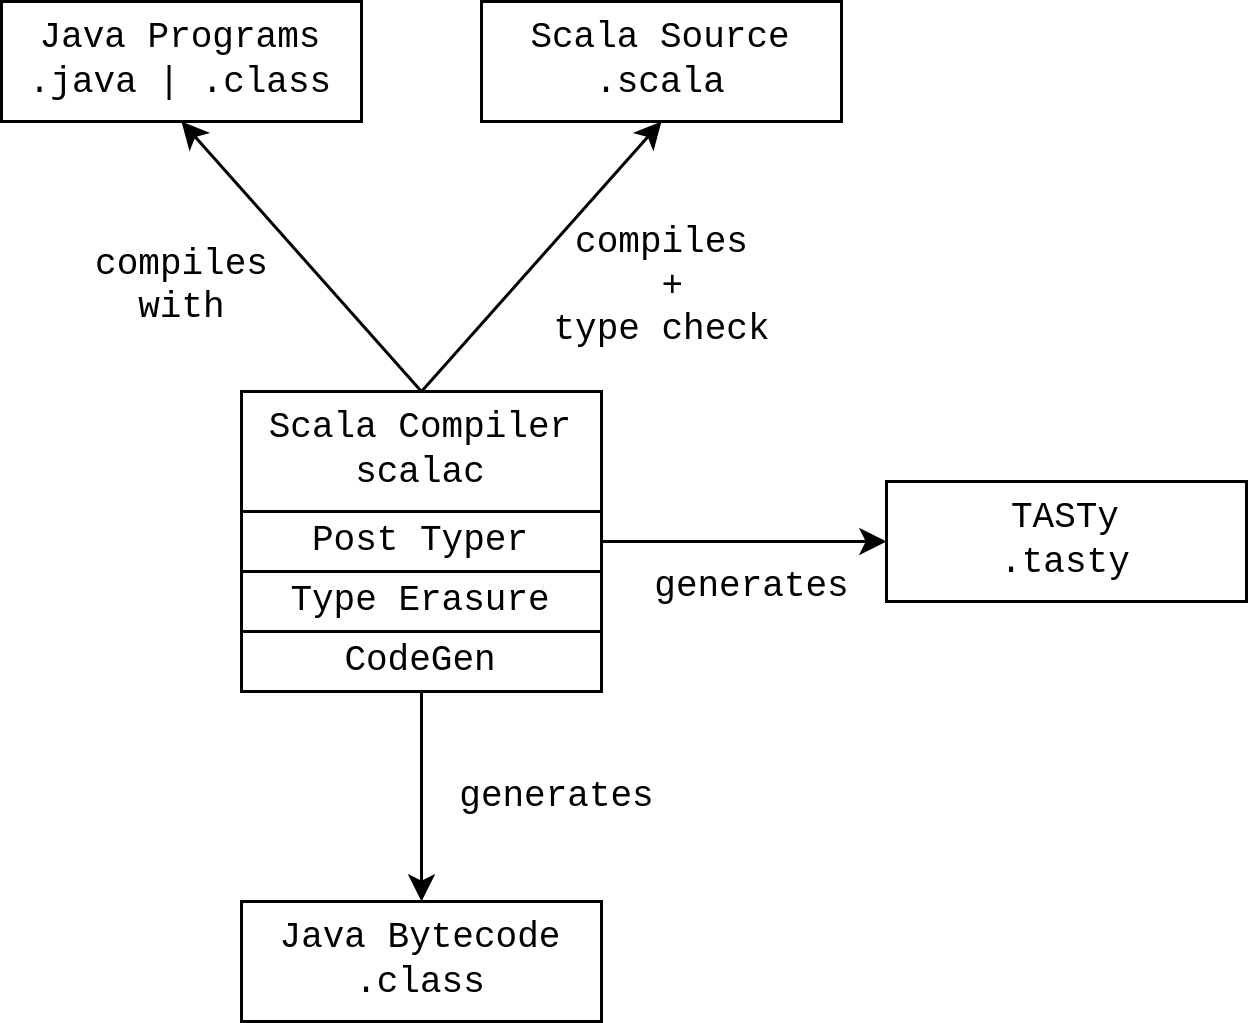
\includegraphics[width=0.4\textwidth]{figures/scala-pipeline.png}
	\caption{TASTy in the context of the Scala compilation pipeline.}
	\label{system:tasty}
\end{figure}

The full TASTy IR can represent all Scala programs.
The Truffle interpreter in this thesis supports a subset sufficient to express the the programs given in figures \ref{example:list-def} and \ref{example:list-impl}.
The TASTy trees used in this thesis can be divided into categories, definitions, terms, and types. 
We give the pseudo implementations of these trees in figures: \ref{tasty:defs}, \ref{tasty:terms}, and \ref{tasty:types}.

\subsection{Definitions}

\begin{figure}[!htb]
	\begin{minted}{scala}
	// Tree representing code written in the source
	trait Tree {
		def symbol: Symbol
	}                         
	trait Statement extends Tree       // Tree representing a statement in the source code
	trait Definition extends Statement // Tree representing a definition in the source code.
		
	// Tree representing a class definition.
	case class ClassDef(
		name:        String,
		constructor: DefDef, 
		parents:     List[Tree], 
		self:        Option[ValDef], 
		body:        List[Statement]
	) extends Definition
	// Tree representing a method definition in the source code
	case class DefDef(
		name:      String, 
		params:    List[ParamClause], 
		returnTpt: TypeTree, 
		rhs:       Option[Term]
	) extends Definition
	// Tree representing a value definition in the source code.
	case class ValDef(name: String, tpt: TypeTree, rhs: Option[Term]) extends Definition
	// Tree representing a type (parameter or member) definition in the source code
	case class TypeDef(name: String, rhs: Tree) extends Definition
	\end{minted} 
	\caption{Pseudocode class definitions for a subset of TASTy trees.}
	\label{tasty:defs}
\end{figure}

A Scala program consists of top level class definition which themselves contain statements.
Statements either represent a declaration inside a class, such as method definitions, or executable code (or terms), which we discuss in section \ref{section:tasty:terms}.
Figure \ref{tasty:defs} provides the pseudo implementations of all definitions in our subset of TASTy.
Every tree has a symbol, which is a unique reference to a definition.
For the use cases in this thesis, most definitions can be translated and be represented by a corresponding implementation in Truffle.
A \scalainline{ClassDef} represents a top level class definition.
A \scalainline{DefDef} tree is the definition of a method inside a class definition.

A \scalainline{ValDef} tree is a context-dependent definition which represents different value definition semantics depending on the tree it is defined in.
A top level \scalainline{ValDef}, that is a \scalainline{ValDef} with no parent represents the \scalainline{object} abstraction in Scala.
The \scalainline{object} abstraction is commonly used to represent the \textit{Singleton} pattern\cite{go4:design-patterns} or as a class-like interface to define static methods.
Consider the \scalainline{Nil} class given in figure \ref{example:nil-impl}, a simplified TASTy-like equivalent would resemble the following:

\begin{figure}[!htb]
	\begin{minted}{scala}
	val Nil = new Nil$
	class Nil$ extends List[Nothing] { ... }
	\end{minted} 
	\caption{Simplified implementation of the \scalainline{object Nil}}
	\label{example:decomp-object}
\end{figure}

A \scalainline{ValDef} tree defined in the \scalainline{body} of a \scalainline{ClassDef} tree represent field definitions.
A \scalainline{ValDef} tree defined in the \scalainline{TermParam} section of a \scalainline{DefDef} tree represent parameter definitions of the method.
A \scalainline{ValDef} tree defined among the statements in a \scalainline{Block} tree is a local variable definition limited to the scope of the block.

Similarly, \scalainline{TypeDef} trees refer to different kinds of definitions depending on their definition site.
A \scalainline{TypeDef} in the body of a \scalainline{ClassDef} refers to a polymorphic class type parameter in our subset of TASTy.
When a \scalainline{TypeDef} is located in the \scalainline{TypeParam} section a \scalainline{DefDef} tree, it refers to a polymorphic method type parameter.
The trees defined here can be used to represent more complex object-oriented and functional abstractions such as nested classes or closures, but they are beyond the scope of this thesis.

Figure \ref{tasty:list} is the TASTy structure of the \scalainline{List} class given in figure \ref{example:list-def}. 
Recall that \scalainline{ClassDef} trees have four structural components, the constructor, the list of parent class definitions, the self type, and the body of the definition.
In this thesis, we will not discuss the self type as it is an abstraction for composition\cite{gilad:mixins}\cite{scala:calculus} and is not relevant for execution.
The list of parents in a class definition in our subset of TASTy is always a singleton.
Note that while the abstract \scalainline{List} class did not explicitly declare a constructor, the compiler autogenerates and inserts the appropriate constructor implementation before emitting TASTy.
Since \scalainline{List} is polymorphic, it contains an inner type definition of its sole type parameter.
This distinction is what makes TASTy a complete IR when compared to the other intermediate representations we will describe later in this chapter.

\begin{figure}[!htb]
	\begin{minted}{scala}
	ClassDef(
		// name 
		"List",
		// constructor
		DefDef("<init>", List(TypeParams(TypeDef("T", TypeBoundsTree(_, _)), TermParams(Nil)), _, None)),
		// parents
		List(Apply(Select(New(_, "<init>"), Nil))),
		// self
		None,
		// body
		List(
			TypeDef("T", TypeBoundsTree(_, _)),
			DefDef("head", Nil, TypeIdent("T"), None),
			DefDef("tail", Nil,Applied(TypeIdent("List"), List(TypeIdent("T"))),None),
			DefDef("length", Nil, TypeIdent("Int"), None),
			DefDef("isEmpty", Nil, TypeIdent("Boolean"), None),
			DefDef(
				"contains",
				List(
					TypeParams(TypeDef("T1", TypeBoundsTree(TypeIdent("T"), _))),
					TermParams(ValDef("elem", TypeIdent("T1"), None))
				),
				TypeIdent("Boolean"),
				None
			)
		)
	)
	\end{minted} 
	\caption{Tree structure for the definition of \texttt{List} . For brevity, we use \textbf{\texttt{\_}} to represent inferred\cite{ml:type-inference} type trees by the compiler.}
	\label{tasty:list}
\end{figure}

Similarly, \scalainline{DefDef} trees also retain their polymorphic properties.
The parameters section of a \scalainline{DefDef} tree is split into two halves.
The type parameter section preserves any polymorphic type parameters in the method definition.
The term parameter section contains the normal value parameters found in a method.
Term parameters may have types which are derived from the type parameter section.

\subsection{Terms}
\label{section:tasty:terms}

\begin{figure}[!htb]
	\begin{minted}{scala}
	// Tree representing an expression in the source code
	trait Term extends Statement {
		def tpe: Type
	}
	// Tree representing a reference to definition      
	trait Ref extends Term             
	
	// Tree representing an assignment lhs = rhs in the source code
	case class Assign(lhs: Term, rhs: Term) extends Term
	// Tree representing new in the source code
	case class New(tpt: TypeTree) extends Term
	// Tree representing a block `{ ... }` in the source code
	case class Block(statements: List[Statement], expr: Term) extends Term
	// Tree representing a while loop
	case class While(cond: Term, body: Term) extends Term
	// Tree representing an if/then/else if (...) ... else ... in the source code
	case class If(cond: Term, thenp: Term, elsep: Term) extends Term
	// Tree representing a return in the source code
	case class Return(expr: Term, from: Symbol) extends Term
	// Tree representing a selection of definition with a given name on a given prefix
	case class Select(qualifier: Term, selector: String) extends Term 
	// Tree representing an application of arguments.
	case class Apply(applicator: Term, arguments: List[Term]) extends Term
	// Tree representing an application of type arguments
	case class TypeApply(fun: Term, args: List[TypeTree]) extends Term
	// Tree representing a reference to definition with a given name
	case class Ident(name: String) extends Ref 
	// Tree representing constant value
	case class Constant(value: Int | ... | String) extends Term 
	\end{minted} 
	\caption{Pseudocode class definitions for a subset of TASTy trees.}
	\label{tasty:terms}
\end{figure}

Figure \ref{tasty:terms} gives the implementation for terms in our subset of TASTy.
Terms represent executable atoms of code which return values.
Terms can be considered analogous to expressions from the abstract syntax trees commonly used for other imperative programming languages.
Our term tree subset of TASTy represents a basic language with support for simple imperative programming with control flow constructs such as branching and loops.
A basic set of object-oriented features are also encapsulated in the tree definitions given above.
The set of object-oriented features include object creation, instance method invocation, and instance field access.
This subset of TASTY is sufficient to represent the creation of polymorphic classes as well as the invocation of polymorphic methods to showcase the examples described in this thesis.

Terms in TASTy also retain their types after type checking by the Scala compiler.
A type for a term describes the type of the value produced by the term.
Terms with no children, such as \scalainline{Ident} trees, are \textit{explicit} typed.
Childrenless terms have their type information encoded in a TASTy file.  
For terms with children, their types are derived from those of their children trees.
Type information for non-leaf term trees is regenerated from term leaves when a TASTy file is read.
In essence, types `flow' upwards from leaf nodes in TASTy to their parent terms until the root term.
The interpreter described in this thesis intreprets a tree where the types for all trees have been regenerated.
We will describe types in detail in the following section.

\subsection{Types and Type Trees}

TASTy encodes Scala programs with two kinds of type information, type trees and types.
Type trees are a subset of trees which represent types as they are declared in Scala source code.
On the other hand, types are the canonical representation of type trees after type checking in the Scala compiler.
Multiple type trees may denote the same underlying type.

\begin{figure}[!htb]
	\begin{minted}{scala}
	// Type tree representing a type written in the source
	trait TypeTree extends Tree {
		def tpe: Type
	}
	
	// Type tree representing a reference to definition with a given name
	case class TypeIdent(name: String) extends TypeTree 
	// Type tree representing a type application
	case class Applied(tpt: TypeTree, args: List[TypeTree | TypeBoundsTree]) extends TypeTree
	// Type tree representing a type bound written in the source
	case class TypeBoundsTree(lo: TypeTree, hi: TypeTree) extends TypeTree
	\end{minted} 
	\caption{Pseudocode class definitions for a subset of TASTy type trees.}
	\label{tasty:type-trees}
\end{figure}

Figure \ref{tasty:type-trees} gives the subset of type trees which we will use in this thesis.
For our purposes, there are only three ways to refer to types.
A \scalainline{TypeIdent} type tree is a reference to a type which is a \scalainline{ClassDef}.
An \scalainline{Applied} type tree represents a type constructor, which accepts type arguments and produces a new type.
For example, the type \scalainline{Cons[T]} would be represented as an applied type tree, where \scalainline{Cons} would the constructor and \scalainline{T} would be the type argument.
A \scalainline{TypeBounds} tree represents the type expression \scalainline{Lo <: T <: Hi}, a constraint where \scalainline{T} must be a subtype of type \scalainline{Hi} and supertype of type \scalainline{Lo}.
Type bounds are typically used to represent declared type parameter constraints, otherwise known as \textit{bounded quantification}\cite{systemF:subtyping}, in polymorphic classes or polymorphic methods.
However, type bounds are also inserted by the Typer because type parameters in TASTy are universally contraints.
A type parameter \scalainline{T} is expanded to \scalainline{Nothing <: T <: Any}, that is the type parameter \scalainline{T} must be a subtype of \scalainline{Any} and a supertype of \scalainline{Nothing}.
In the context of this thesis, we can use subtype to mean \textit{subclass of} and supertype to mean \textit{superclass of}.
Practically, this means the type parameter \scalainline{T} has no constraints since \scalainline{Any} is the super type of all types and \scalainline{Nothing} is the subtype of all types.

\begin{figure}[!htb]
	\begin{minted}{scala}
	trait Type                           // A type, type constructors, type bounds
	trait NamedType extends Type         // Type of a reference to a type or term symbol
	case class TypeRef extends NamedType // Type of a reference to a type symbol
	case class AppliedType extends Type  // A higher kinded type applied to some types T[U]
	case class TypeBounds extends Type   // Type bounds
	\end{minted} 
	\caption{Pseudocode class definitions for a subset of TASTy type trees.}
	\label{tasty:types}
\end{figure}

Figure \ref{tasty:types} is set of types used in our subset of TASTy.
In most cases in our subset of TASTy, the type trees have a corresponding type of the same name.
However, the \scalainline{NamedType} does not appear in type trees as they are predominantly used to type terms.
The \scalainline{TypeRef} type is a reference to a \scalainline{ClassDef} tree or a type parameter \scalainline{TypeDef}.

In the Scala compilation pipeline, TASTy is eventually simplified and transformed by the Scala compiler to produce Java bytecode. 
In chapter \ref{chapter:implementation}, We will go over each tree before such transformations and their relevance for execution in our interpreter .

\section{Java Bytecode}

Java bytecode is a portable and compact intermediate language and instruction set used by the Java Virtual Machine to execute programs.
Java bytecode can be considered similar to an assembly language, where programs are represented as sequences of atomic instructions which manipulate a stack or registers.
The type system in Java bytecode can describe primitive values such as \javainline{int} and references to objects such as \javainline{String}.
As bytecode is intended to be simple for execution, it is not possible to represent polymorphic programs fully in Java bytecode.

Types in TASTy are not immediately compatible with types available in Java bytecode.
Scala's type semantics must be eliminated from programs by the compiler before Java bytecode of the program can be emitted.
The resulting Java bytecode is considered an \textit{incomplete} IR of Scala source programs, as the type information found in the program source or inferred from compilation is no longer present.
This becomes a particular drawback for executing Scala programs on the JVM because speculative optimizations are unable to incorporate source level semantics.

\begin{figure}[!htb]
	\begin{minted}{scala}
	aload_0
 	astore_2
	aload_2
	invokevirtual #44 // List.isEmpty:()Z
	ifne          30
	aload_2
	invokevirtual #46 // List.head:()Ljava/lang/Object;
	aload_1
	invokestatic  #52 // Method scala/runtime/BoxesRunTime.equals:(Ljava/lang/Object;Ljava/lang/Object;)Z
	ifeq          22
	iconst_1
	ireturn
	aload_2
	invokevirtual #53 // List.tail:()LList;
	astore_2
	goto          2
	iconst_0
	ireturn
	\end{minted}
	\caption{Java bytecode of \texttt{Cons.contains}}
	\label{example:contains-bytecode}
\end{figure}

Figure \ref{example:contains-bytecode} is the Java bytecode of the \scalainline{contains} defined at line 4 in figure \ref{example:cons-impl}.
Typical control flow elements of Scala programs such as if terms and while terms have been converted into branch and jump instructions.
Notice that there are no polymorphic type parameters in the description of classes nor in the invocation of polymorphic methods present in the bytecode.
In particular, notice the equality comparison in line 7 of figure \ref{example:cons-impl} is actually a method invocation (instruction 14 in figure \ref{example:contains-bytecode}).
As the Scala compiler is unable to determine the type of a polymorphic type parameter during complilation time, it is unable to select a Java bytecode instruction which implements polymorphic comparison.
Instead, a bridge method part of the Scala standard library is responsible for handling polymorphic operations which operate on both reference and primitive types during runtime.
In the next section, we describe the process which transforms Scala programs to a reprensentation amenable for Java bytecode generation and the necessary additional runtime overhead associated with this transformation.

\section{Type Erasure}
\label{background:type-erasure}

Type erasure\cite{java:generics} is a transformation which converts polymorphic classes and methods in Scala to monomorphic classes and methods. 
This conversion is necessary because the JVM does not support polymorphic classes during runtime.
Erasure ensures that any given polymorphic class and method has a single representation in practice.
Type erasure is a crucial part of Scala compilation that renders TASTy incomplete.
Figure \ref{example:erase-cons} shows the \scalainline{Cons} class after type erasure.

\begin{figure}[!htb]
	\begin{minted}{scala}
	case class Cons(head: Any, tail: List) extends List {
		override def length: Int = 1 + tail.length
			
		override def contains(elem: Any): Boolean = {
			var these: List = this
			while (!these.isEmpty) 
			if (these.head == elem) return true
			else these = these.tail
			false
		}
			
		override def hashCode(): Int = {
			var these: List = this
			var hashCode: Int = 0
			while (!these.isEmpty) {
				val headHash = these.head.##
				if (these.tail.isEmpty) hashCode ||= headHash
				else hashCode |= headHash >> 8
				these = these.tail	
			}
			hashCode
		}
	}		
	\end{minted}
	\caption{\scalainline{Cons} class after type erasure}
	\label{example:erase-cons}
\end{figure}

The polymorphic \scalainline{Cons} class has all type parameters in its class definition \textit{erased} and replaced by the \scalainline{Any} type.
The \scalainline{Any} type is a Scala platform-independent\cite{scala:overview} abstract type representing the supertype of primitive and reference types.
In Java bytecode, the {Any} type is compiled to the \scalainline{Object} type, the supertype of all reference types on the JVM.

While type erasure simplifies classes for runtime, the Scala compiler must resolve the incompatibility of operations between primitives types and reference types on the JVM\cite{java:vm-spec}.
In order for primitive types to have a uniform representation compatible with reference types, primitive types are encapsulated into corresponding boxed classes whose objects are passed by reference.
For example, \javainline{java.lang.Integer} is a class with an \scalainline{Int} field.
In a polymorphic context in which a type variable has been replaced by the reference type \javainline{Object}, an \scalainline{Int} value is not passed directly, but by reference to an object of class \javainline{Integer} that contains the primitive value.
The set of operations introduced by the compiler whenever a primitive value is accessed under a polymorphic context is known as \textit{autoboxing}\cite{java:autoboxing}. 
Autoboxing can be divided into two operations.
\textit{Boxing} occurs when a primitive value must be used where a polymorphic value is expected.
\textit{Unboxing} occurs when a polymorphic value must be used where a primitive value is expected.
Figure \ref{example:autoboxing} shows a simple example of inserted autoboxing operations when using the polymorphic \scalainline{Cons} class after type erasure.

\begin{figure}[!htb]
	\begin{minted}{scala}
	// Before type erasure 	
	val lst: List[Int] = Cons(1, Nil)
	val head: Int = lst.head
	// After type erasure
	val lst: List = Cons(box(1), Nil)
	val head: Int = unbox(lst.head) 
	\end{minted}
	\caption{Example of autoboxing introduced for a list}
	\label{example:autoboxing}
\end{figure}

The \scalainline{head0} field inside the \scalainline{Cons} class after erasure is no longer polymorphic and instead has the type \scalainline{Any}. 
The integer value of \scalainline{1} which is passed into the class constructor for the list is boxed and the primitive value is wrapped as an instance of its boxed class.
Similarly, when the \scalainline{head0} field of the instance is read and stored into a local variable, an unboxing operation occurs which extracts the primitive value out of its wrapper instance.
In the Scala collections library, a set of commonly used polymorphic data structures, autoboxing operations are frequent and necessary.
The computational overheads of autoboxing operations on programs which make substantial use of polymorphic collections, especially the Scala standard library, is significant\cite{scala:collections-optimization}.
The elimination of this overhead through optimizing autoboxing operations is one of the central goals of this thesis.
In addition to this direct overhead, autoboxing is a significant indirect source of overhead which makes the analysis of programs using primitive values in a polymorphic context and thus inhibits many significant compiler optimizations.

\section{GraalVM}

GraalVM\cite{java:graalvm} is an implementation of a JVM.
Traditionally, the JVM is responsible for the majority of the performance optimizations in Java programs\cite{java:hotspot} through \acrfull{jit} compilation.
JIT compilation is an adaptive optimization which occurs during program execution.
JIT compilation is concerned with optimizing and eliminating \textit{hotspots} or portions of the program which are executed most frequently.
JIT compilers\cite{java:sablevm}\cite{java:jikesrvm} employ a range of \textit{speculative} techniques to transform the program under optimization.
Speculative optimizations use information collected during program execution, otherwise known as \textit{profiling}. 
Assumptions are then made about gathered profiling data in order to generate high-performance native machine code.
A key aspect of speculative optimizations using assumptions is that optimizations may be undone when their underlying assumptions are violated.
This enables the JIT compiler to optimize programs without the need to statically prove assumptions hold in every execution path.

While other implementations of Java virtual machines were designed specifically for Java, GraalVM was designed from the onset to be \textit{language-independent}.
GraalVM can be divided into two major components of interest. 
The first is \textit{Graal}, a language-agnostic JIT compilation infrastructure which handles speculative optimizations and generation of high-performance machine code.
The second is \textit{Truffle}, a framework for translating the semantics of a source language, also called a \textit{guest language}, to take advantage of the Graal infrastrucure.

\begin{figure}[!htb]
	\centering
	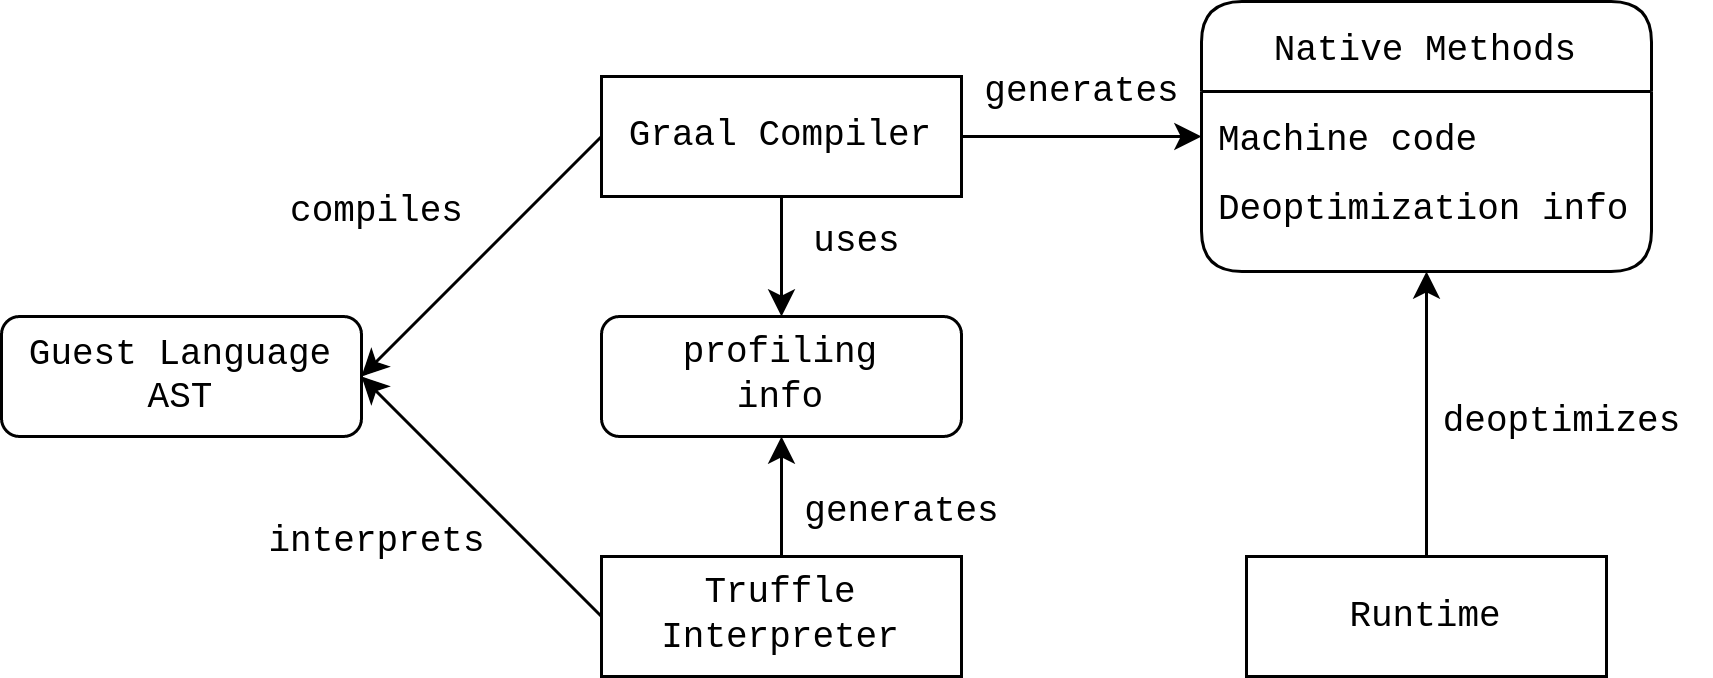
\includegraphics[width=0.5\textwidth]{figures/graalvm-pipeline.png}
	\caption{GraalVM overview\cite{graalvm:ir}.}
\end{figure}

This thesis makes substantial of both components of GraalVM to create a runtime for Scala programs using TASTy.
The runtime is able to incorporate source level information for speculative optimizations.


\subsection{Graal}

GraalVM incorporates an existing implementation of a JVM\cite{java:hotspot} for the actual execution of programs.
Graal is \textit{only} the general-purpose just-in-time compilation infrastructure which optimizes the programs to be executed.
Graal is general-purpose in that it conducts analysis and optimization on the same intermediate representation, \textit{Graal IR}, regardless of the original source language.
Notably, most implementations of a source language utilizing GraalVM have an implementation in Truffle, Java is an exceptional case.
In addition to a Truffle interpreter for Java bytecode\cite{graalvm:espresso}, there is a direct translator for Java programs in GraalVM which parses Java bytecode into Graal IR.

Graal IR\cite{graalvm:ir}\footnote{Given the number of intermediate representations introduced thus far, we promise this is the last one} is an IR which is suitable for speculative optimizations while still retaining information from the Truffle guest language AST.
Graal IR is based on the \textit{sea of nodes} concept\cite{click:sea-of-nodes} and satisfies the \textit{static single-assignment}\cite{ssa} property.
A sea of nodes is an abstraction based on a directed graph structure which relates the control flow graph\cite{allen:ctrl-flow-analysis} of a program to its data flow graph\cite{allen:data-flow-analysis}.
An intermediate representation is in single-static assignment form when each variable is declared once and every use of a variable occurs immediately after its declaration\cite{johnson:use-def-chains}.

GraalIR enables Graal to speculatively compile only the \textit{hot} branches\cite{graalvm:speculative-ir}, or branches that are most frequently taken, in the control flow portion of the IR and their transitive data dependencies.
When a compiled program violates any of its underlying assumptions, execution is \textit{deoptimized}\cite{self:deoptimization} and the program resumes execution in its uncompiled format.
Deoptimization occurs when the compiled program is no longer considered stable and therefore is invalid.
Graal automatically inserts \textit{guard nodes} into the IR, which are conditional checks which validate that speculative assumptions used to compile the program still hold.
Deoptimization is part of an execution loop between Graal and Truffle which allows GraalVM to aggressively adapt and speculate to find the best optimization in a dynamic execution environment.

\smartdiagramset{
	text width=2.75cm,
	uniform color list=white for 3 items,
	uniform arrow color=true,
	arrow color=black,
}
\begin{figure}[!htb]
	\centering
	\scalebox{0.7}{
		\smartdiagram[circular diagram:clockwise]{
			Node rewriting,
			Partial evaluation,
			Deoptimization
	}}
	\caption{Adaptive optimization loop of GraalVM}
	\label{diagram:graal-loop}
\end{figure}

\subsection{Truffle}

Truffle is a framework for implementing an interpreter embedded into GraalVM.
Truffle differs signficantly from other implementations of interpreters.
Interpreters can usually be divided into two subsets: tree interpreters and bytecode interpreters.
Tree interpreters transform program source into an abstract syntax tree which is then executed in post-order, children nodes are executed before their parents.
Abstract syntax tree interpretation has the added benefit of executing an intermediate representation which is quite close to the program source representation and is therefore more amenable to program optimization.
In contrast, bytecode interpreters such as the JVM, execute a vastly simplified representation of programs.
While interpreters of bytecode programs tend to be faster than their tree counterparts, the absence of detailed source information such as types often makes program optimization difficult.
The challenge of efficiently executing bytecode while retaining the ability to optimize them effectively using source program information is particularly difficult for Scala on the JVM. 

\begin{figure}[!htb]
	\begin{minted}{scala}
	abstract class EqualsNode extends BinaryOpNode {
		@Specialization
		def equalsInt(lhs: Int, rhs: Int): Boolean = lhs == rhs
		
		@Specialization(replaces="equalsInt")
		def equals(lhs: Any, rhs: Any): Boolean = if (lhs == null) rhs == null else lhs.equals(rhs)
	}
	\end{minted}
	\caption{Pseudocode for a Truffle node implementation of an equality which supports node rewriting.}
	\label{example:node-rewriting}
\end{figure}

Truffle is an atypical tree interpreter in that it combines the definition, execution, and optimization of an abstract syntax tree structure into a single abstraction.
While the structure of input programs in other interpreters is independent of the implemenation of the interpreter, a Truffle interpreter is integrated into the structure of its input.
By defining execution semantics inside the abstract syntax tree to be executed, an interpreter is essentially derived from the implementation of its input tree structure.
The execution semantics of the AST are additionally augmented with the Truffle \acrfull{dsl}, which allows such trees to be \textit{self-optimizing}.
The Truffle DSL is a mechanism to allow a \textit{guest language} to embed semantics into a Truffle AST for optimization.
A guest language is a set of semantics, most commonly a programming language, which is described by a Truffle AST.
In this thesis, the guest language which our Truffle AST encodes and executes is TASTy (which represents Scala).

\begin{figure}[!htb]
\begin{minted}{java}
	@GeneratedBy(AnyEqNode.class)
	public final class AnyEqNodeGen extends AnyEqNode {
		@Child
		private TermNode lhs_;
		@Child
		private TermNode rhs_;
		@CompilationFinal
		private int state_0_;
		
		private AnyEqNodeGen(TermNode lhs, TermNode rhs) {
			this.lhs_ = lhs;
			this.rhs_ = rhs;
		}
		
		public Object execute(VirtualFrame frame) {
			int state = this.state_0_;
			return (state & 2) == 0 && state != 0 ? 
				this.execute_int_int0(state, frame) : 
				this.execute_generic1(state, frame);
		}
\end{minted}
\end{figure}

During execution of the AST, profiling information collected from the interpreter is used to drive \textit{node rewriting}.
While Graal is language-agnostic, Truffle is able to exploit guest language semantics for dynamic optimizations.
This process of replacing nodes in the AST with better, specialized guest language counterparts in Truffle is called node rewriting.
Node rewriting makes Truffle abstract syntax trees self-optimizing and serves two purposes.
The first is to dynamically incorporate guest language semantics into the executing program.
The second is to augment the AST for more efficient JIT compilation.
The nature of compiler optimizations require that programs are incrementally simplified in order to be optimized.
While such types of optimizations are widely applicable to many languages using the JVM, node rewriting is a high-level language-specific optimization which occurs \textit{before} such simplifications.

Figure \ref{example:node-rewriting} demonstrates an example of a node which can be rewritten.
The node declares semantics of the equality operation between integers and values of type \scalainline{Any}.
This equality node has semantics for every type because the \scalainline{Any} type is the super type of all types in Scala .
A Truffle node which can be rewritten starts off in the uninitialized state.
When both the left and right hand side operands are integers, the node is rewritten to \javainline{equalsInt} state.
When arguments of any other combination of types are detected, either in the uninitialized state or the \javainline{equalsInt} state, the node is rewritten to the \javainline{equals} state.

After node rewriting, Graal JIT compiles Truffle ASTs into native machine code using \textit{partial evaluation}.
Partial evaluation is a program optimization technique for specializing a program (code) for a given input (data)\cite{futamura:partial-eval}.
In the context of Truffle, this means specializing an AST node (code) based on the values (or types of values) produced by their children nodes (data)\cite{truffle:partial-eval}.
We can say that the partial evaluation of an AST  will produce an AST which is \textit{specialized} for a particular set of values, or more commonly in our case, a particular set of types.
If a frequently executed Truffle AST cannot be rewritten further, it is considered \textit{stable} for JIT compilation into native machine code.  
The sequence of optimizations given in figure \ref{diagram:graal-loop}, node rewriting, partial evaluation into machine code, and deoptimization is the advantage that a TASTy Truffle interpreter has over the traditional JVM bytecode interpreter for Scala.
Truffle allows for the incorporation of source-level type information into the just-in-time compilation loop.
In this thesis, we will focus heavily on using node rewrites in the execution of TASTy with type information to augment JIT compilation.



%======================================================================

\chapter{Implementation}
\label{chapter:implementation}
% \epigraph{The best presents don't come in boxes.}{Bill Watterson}
% \epigraph{Typing is no substitute for thinking.}{Dartmouth Basic manual, 1964}

This chapter is divided into two halves which detail the implementation of a Truffle interpreter and extensions for parametric polymorphism.
The first half of this chapter will describe the methods used to transform TASTy to make it suitable for a Truffle interpreter, \textsc{TastyTruffle}, \textit{without} polymorphism.
In particular, the first section covers how to translate the organization of data and code in the \scalainline{DefDef}, \scalainline{ClassDef}, and \scalainline{Term} tree nodes into a Truffle implementation which is amenable to execution and JIT optimization.
The second half of this chapter will then discuss extensions to our implementation support parametric polymorphism and cover the techniques we use to specialize nodes to eliminate autoboxing in the presence of polymorphism. 

\section{The Monomorphic Interpreter}
\label{impl:section:monomorphic}

Scala programs in \acrshort{tasty} format are unsuitable for execution in a Truffle interpreter. 
Programs in TASTy must be parsed and transformed into an executable representation in Truffle.
This involves translating the TASTy tree structure into a simpler, but semantically equivalent Truffle AST.
For the rest of this thesis, we refer to the Truffle AST of TASTy as \textit{TastyTruffle IR}.
As TASTy represents a Scala program close to its equivalent source representation, canonicalization compiler passes (see appendix \ref{appendix:dotty-phases}) that would otherwise normalize the IR are not present. 
Instead, we implement TastyTruffle IR to represent a canonicalized executable intermediate representation which can later be specialized on demand. 

\begin{figure}[!htb]
	\begin{minted}{scala}
	def evaluate(tree: Tree): Object = tree match {
		case vdef: ValDef   => 
			lazy val obj = initializeObject(vdef)
			registerObject(vdef.symbol, obj)			
		case cdef: ClassDef => 
			registerShape(cdef.tpe, parseClassDef(cdef))	
		case _ => ()
	}
	\end{minted}
	\caption{Pseudocode to evaluate every top level tree.}
	\label{impl:top-level}
\end{figure}

Figure \ref{impl:top-level} gives an evaluation loop that is common in other interpreters in the context of this one.
A top level tree is any tree without a parent.
In our subset of TASTy, a top level tree may be a \scalainline{ValDef} (a singleton object) or a \scalainline{ClassDef}.
Here we only present the pseudocode sufficient to traverse a program in TASTy. 
Each top level definition is parsed and saved.
Note that we intentionally omit \textit{how} to execute the program.
Entry points in \scalainline{TASTy} are defined by a special method \scalainline{main}.
As multiple entry points may exist in a given program, we consider the selection of entry points an implementation-specific detail.
In the following sections, we will describe the individual types of TASTy nodes and why some are directly unsuitable for execution and how to simplify their semantics for execution.

\subsection{Converting the \texttt{DefDef} tree into a Truffle Root Node}
\label{impl:subsection:defdef}

In this section, we describe the conversion of \scalainline{DefDef} trees to \textit{root nodes}.
\scalainline{DefDef} trees are the primary structure which organizes code (terms) in TASTY.
Root nodes represent the root of an executable Truffle AST, the primary abstraction which organizes code in Truffle.
In our case, root nodes are the Truffle analog of a \scalainline{DefDef}.
Each root node has a corresponding \textit{call target}, which is used for invocation of the root node.
Call targets are the primary compilation unit for Graal.
A compilation unit is an organization of code which can be independently compiled.
A root node is automatically instrumented\cite{profiling:atom} to profile its number of invocations. 
When a root node has been frequently invoked inside the interpreter, it is JIT compiled into machine code by Graal.
Subsequent invocations of the call target will then use the more efficient compiled root node.

\begin{figure}[!htb]
	\begin{minted}{scala}
	abstract class RootNode(desc: FrameDescriptor) {
		def execute(frame: VirtualFrame): Object
		def getCallTarget: CallTarget
	}
	\end{minted}
	\caption{Pseudocode of a root node.}
	\label{example:root-node}
\end{figure}

Figure \ref{example:root-node} gives a simplified implementation of a root node.
Each root node in Truffle has a \textit{frame descriptor} and execution semantics.
A guest language must subclass and implement its own root node in order to enable function invocation semantics.

A frame descriptor describes guest language variables which are in scope during execution.
The abstract \javainline{execute} method describes the invocation behaviour of a root node.
When a root node is executed, it always supplied with a \textit{frame}.
A frame contains the arguments supplied during invocation and storage slots for local variable definitions in the body of the method.
By default, all frames start off \textit{virtual}.
Virtual frames are Truffle abstractions that provide guest languages an opportunity to exploit escape analysis.
Escape analysis\cite{escape-analysis} reasons about the dynamic scope of object allocations. 
Truffle and Graal both exploit the observations of \textit{Partial Escape Analysis}\cite{java:partial-escape-analysis}, a path-sensitive variant of escape analysis, to enable the following optimizations for guest languages:

\begin{description}
	\item[Region Allocation\cite{java:escape-analysis}\cite{tofte:region-memory}] The substitution of heap allocations with stack allocations to eliminate unnecessary garbage collection.
	\item[Scalar Replacement\cite{java:escape-analysis-optimizations}] The complete elimination of an object allocation, where the fields of the replaced object are substituted by local variables.
\end{description}

The virtual frame abstraction allows guest languages to read and write to a frame without the requirement to optimize their object allocations.
Instead, escape analysis and subsequently scalar replacement is responsible for optimizing guest language object allocations during partial evaluation. 

\begin{figure}[!htb]
	\begin{minted}{scala}
	class DefDef(_: String, params: List[ParamClause], _: TypeTree, rhs: Option[Term]) extends Definition	
	\end{minted}
	\caption{Defintion of a \texttt{DefDef} tree with names of less important members replaced with \texttt{\_}}
	\label{recall:defdef}
\end{figure}

A further simplified definition of a \scalainline{DefDef} tree is provided in figure \ref{recall:defdef}.
In this section, we focus on two members of a \scalainline{DefDef} trees.
The parameters of a \scalainline{DefDef} tree are given by the \scalainline{params} field.
In practice, the type of a \scalainline{ParamClause} is an alias for the union type \scalainline{TypeParams {|} TermParams}, so we omit the \scalainline{ParamClause} definition.
A \scalainline{DefDef} tree will have a parameter section for type parameters when they are polymorphic and will always have term parameters section.
\scalainline{DefDef} trees may optionally have a body defined in the \scalainline{rhs} field.
When trees do not have a body defined, they are abstract method definitions and do not have  corresponding root node in Truffle.
We will only consider non-abstract method definitions which have a body (a term) defined to be executable.
We will cover the parsing of terms into nodes for execution in detail after section \ref{impl:subsection:classdef}

\begin{figure}[!htb]
	\begin{minted}{scala}
	object FrameSlotKind extends Enumeration {
		type FrameSlotKind = Value
		val Object, Long, Int, Double, Float, Boolean, Byte = Value
	}	
		
	def getFrameSlotKind(tpe: Type): FrameSlotKind = 
		if (tpe.isPrimitive) 
			getPrimitiveSlotKind(tpe) // Int => FrameSlotKind.Int, ..., Double => FrameSlotKind.Double
		else  
			FrameSlotKind.Object
	\end{minted}
	\caption{Simplified implementation of \scalainline{FrameSlotKind}}
	\label{impl:frameslot-kind}
\end{figure}

Each value definition in the parameters of a \scalainline{DefDef} will have a corresponding frame slot in its parent frame descriptor. 
A frame slot references a unique frame value in the context of a root node.
Truffle permits each frame slot in a frame descriptor be described by a \textit{frame slot kind}.
In Truffle, there is a corresponding frame slot kind for reference types and each \acrshort{jvm} primitive type. 
Pseudocode of a frame slot kind and a method to convert a type into a slot kind is given in \ref{impl:frameslot-kind}.

Truffle profiles frame accesses in order to minimize the amount of autoboxing which occurs when reading from frame slot with an \javainline{Object} kind. 
To eliminate unnecessary specialization of frame accesses where types are monomorphic and statically refer to a primitive type, a parameter is assigned the matching primitive frame slot kind in the frame descriptor. 
In cases where the type is not a primitive type or a polymorphic applied type, e.g. \scalainline{List[T]} but not \scalainline{T}, we assign its frame slot the \scalainline{Object} kind.
Otherwise, the type is a polymorphic parameter which \textit{could} resolve to a primitive type and the frame slot kind cannot be resolved statically.
We will defer discussion on how to handle parameters of such polymorphic types that cannot be resolved statically until section \ref{implementation:specialization}.

\begin{figure}[!htb]
	\begin{minted}{scala}
	case class LocalVal(slot: FrameSlot, kind: FrameSlotKind)
		
	class DefDefNode(desc: FrameDescriptor, params: Array[LocalVal], body: TermNode) extends RootNode(desc) {
		override def execute(frame: VirtualFrame): Object = {
			copyArgumentsToFrame(frame)
			try {
				body.execute()
			} catch {
				case ex: ReturnException => ex.getValue
			}
		}	
			
		def copyArgumentsToFrame(frame: VirtualFrame): Unit = 
			for ((param, arg) <- params zip frame.getArguments) 
				param.kind match {
					case FrameSlotKind.Int =>
						frame.setInt(param.slot, arg.asInstanceOf[Int])
					...
					case FrameSlotKind.Double =>
						frame.setDouble(param.slot, arg.asInstanceOf[Double])	
					case _ =>
						frame.setObject(param.slot, arg)
				}
	}
	\end{minted}
	\caption{Pseudocode for \scalainline{DefDefNode} and \scalainline{Parameter}}
	\label{impl:defdefnode}
\end{figure}

Figure \ref{impl:defdefnode} provides the implementation of the \scalainline{DefDefNode} and its parameters, the root node equivalent of a \scalainline{DefDef}.
The execution of a \scalainline{DefDefNode} is divided into two stages, argument preparation and execution.
First, the arguments of the frame constructed during invocation (see \ref{impl:subsection:apply}), are copied into their respective parameter frame slots.
Frames contains separate regions for values of each frame slot kind.
Based on the frame slot kind prescribed to a parameter, we copy each argument into the appropriate frame slot region.
Storing parameters in this manner eliminates any unnecessary unboxing which would otherwise occur during a frame access.
After arguments are copied into the frame, their values become available for access during the execution of the body.
The body of a \scalainline{DefDefNode} is then executed and its computed value returned.

\begin{figure}[!htb]
	\begin{minted}{scala}
	def parseDefDef(ddef: DefDef): DefDefNode = {
		val desc = new FrameDescriptor
		val parameters = self :: ddef.params.map {
			case vdef: ValDef => createParameter(vdef, desc)
		}
			
		val body = parse(ddef.rhs)
		new DefDefNode(desc, parameters, body)
	}
		
	def createParameter(vdef: ValDef, desc: FrameDescriptor): LocalVal = {
		val kind = getFrameSlotKind(vdef.tpt.tpe)
		val slot = desc.addSlot(kind)
		Parameter(slot, kind)
	}
	\end{minted}
	\caption{Pseudocode for parsing \scalainline{DefDef} into \scalainline{DefDefNode}}
	\label{impl:parse-defdef}
\end{figure}

Figure \ref{impl:parse-defdef} provides a summary on parsing a \scalainline{DefDef} tree into its Truffle equivalent \scalainline{DefDefNode}.
Frame slot and a frame slot kinds provide an abstraction for parameters and arguments to be resolved before the execution of the main body in a \scalainline{DefDefNode}.
In addition to the parameters which are explictly present in TASTY, the root node will have additional parameter which represents the receiver of the method.
The receiver is an object instance whose class definition owns the method being invoked.
In Scala, every method invocation has a receiver.
In TASTy, this translates to every \scalainline{DefDef} is owned by a \scalainline{ClassDef}.
In the next section, we detail how to organize call targets in Truffle by using \scalainline{ClassDef} trees.

\subsection{Deriving Shapes from \texttt{ClassDef} trees}

\begin{figure}[!htb]
	\centering
	\begin{subfigure}[b]{0.48\textwidth}
	\begin{minted}{scala}
	class ClassDef(
		name:        String,
		constructor: DefDef, 
		parents:     List[Tree], 
		_:           Option[ValDef], 
		body:        List[Statement]
	) extends Definition
		\end{minted}
	\caption{Pseudocode of a \scalainline{ClassDef}.}
	\label{recall:classdef}
	\end{subfigure}
	\hfill
	\begin{subfigure}[b]{0.48\textwidth}
	\begin{minted}{scala}
	class ClassShape(
		symbol:  Symbol,
		parents: Array[Symbol],
		fields:  Array[Field]
		methods: Map[MethodSignature, CallTarget]
		vtable:  Map[MethodSignature, Symbol]
	)
	\end{minted}
	\caption{Pseudocode of a shape for a \scalainline{ClassDef}.}
	\label{impl:classshape}
	\end{subfigure}
\end{figure}

\scalainline{ClassDef} tree define the layout of an object in TASTy.
The layout of a object dictate the values which an object instance stores as well the methods which can be invoked on an object instance.
The data layout of an object in a Truffle interpreter is described by a \textit{shape}\cite{self:prototypes}\cite{truffle:object-model}.
Shapes are a language-agnostic model for defining the properties of a object instance in Truffle.
A property in a shape describes one member of an object instance; it has an identifier and a value.
A Truffle object instance consists of \textit{object storage}, which contains instance-specific data, and its shape.
Shapes map property identifiers to object storage locations; guest languages interface with object storage indirectly through properties.
In this thesis we use a \textit{static shape}, an immutable variant of a shape.
Normally, shapes are mutable and their list of properties may change throughout the lifetime of a program\cite{truffleruby:object-model}.
However, programs which dynamically change the layout of their objects\cite{java:reflection} are out of the scope of this thesis.

\begin{figure}[!htb]
	\begin{minted}{scala}
	def parseClassDef(cdef: ClassDef): ClassShape = {
		val parents = cdef.parents.map(_.symbol)
		
		val fields = cdef.body map {
			case vdef: ValDef => generateField(vdef)	
		}
		
		val methods = (cdef.constructor :: cdef.body) map {
			case ddef: DefDef => ddef.symbol.signature -> parseDefDef(ddef)
		}
		
		val vtable = cdef.symbol.methodMembers map {
			symbol => symbol.signature -> symbol
		}
	
		new ClassShape(cdef.symbol, parents, fields, init ++ methods, vtable)
	}

	def generateField(vdef: ValDef): Field = vdef match {
		case ValDef(_: String, tpt: TypeTree, rhs: Option[Term]) => new Field(vdef.symbol, )
	}
	\end{minted}
	\caption{Pseudocode to convert a \scalainline{ClassDef} into a \scalainline{ClassShape}.}
	\label{impl:parse-classdef}
\end{figure}

Recall the definition of a \scalainline{ClassDef} in figure \ref{recall:classdef}.
Each \scalainline{ClassDef} tree can be parsed into a corresponding \scalainline{ClassShape}, given in Figure \ref{impl:classshape}.
Figure \ref{impl:parse-classdef} provides a very simplified implementation of the parsing steps to transform a \scalainline{ClassDef} into a \scalainline{ClassShape}.
The \scalainline{name} parameter of \scalainline{ClassDef} alone is insufficient to be used as an identifier for a \scalainline{ClassShape}.
Names do not disambiguate between classes of the same name declared in different packages.
Instead, we used the symbol of the \scalainline{ClassDef} tree as the identifier for the \scalainline{ClassShape}.
For the remainder of this thesis, we will use a \scalainline{ClassInstance} to refer to an object instance with properties described by a \scalainline{ClassShape}.

\begin{figure}[!htb]
	\begin{minted}{scala}
	class Field(symbol: Symbol, tpe: Type) extends StaticProperty {
		override def getId: String = symbol.name
			
		def get(instance: Object): Any = 
			if (tpe == Int) getInt(instance)
			else if ...
			else if (tpe == Double) getDouble(instance)
			else getObject(instance)
	
			
		def set(instance: Object, value: Any): Unit = 
			if (tpe == Int) setInt(instance, value.asInstanceOf[Int])
			else if ...
			else if (tpe == Double) setDouble(instance, value.asInstanceOf[Double])
			else setObject(instance, value)	
	} 
	\end{minted}
	\caption{Pseudocode of the field property.}
	\label{impl:field}
\end{figure}

A \scalainline{ValDef} tree in the body of a \scalainline{ClassDef} translates to a field definition in the \scalainline{ClassShape}.
A \scalainline{ClassShape} has an collection of fields, which implement the static shape property.
Figure \ref{impl:field} gives our implementation of a field.
Fields define operations to read and write from the object storage on a \scalainline{ClassInstance}.
Like frames with frame slot kinds, object instances in Truffle have separate regions for storing values of each primitive type and one for reference types.
Following the same rules with types and frame slot kinds described in section \ref{impl:subsection:defdef}, the data access of a field depends on the type of the \scalainline{ValDef} tree from which the field originates.
The remaining members of a \scalainline{ClassShape} do not describe data which has to be stored in the object storage of a \scalainline{ClassInstance}.

\begin{figure}[!htb]
	\begin{minted}{scala}
	case class MethodSignature(symbol: Symbol, params: Int, types: Array[Type])
	\end{minted}
	\caption{Pseudocode of a method signature.}
	\label{impl:method-signature}
\end{figure}

After the constructor and the \scalainline{DefDef} statements of a \scalainline{ClassDef} are converted into root nodes, they are stored in the \scalainline{ClassShape} mapped by a method signature.
The pseudocode for a method signature is given in figure \ref{impl:method-signature}.
Method signatures disambiguate method invocations in the presence of \textit{ad hoc polymorphism}\cite{strachey:fundamental-concepts}, where methods share the same name but have different arguments.
When combined with parametric polymorphism, method signatures must also be able to disamibguate between methods sharing the same name but having different type parameters.
However, method signatures do not have to disambiguate between different type parameters by name, only the number of type parameters that a method has.
Because type erasure erases polymorphic type parameters from methods, methods which share the same number of parameters as well as the same arguments will conflict and therefore are invalid.
As previously mentioned, methods are shared between all \scalainline{ClassInstance} objects with the same shape, call targets are stored on the shape itself.

Often a shape will not contain the call target referenced by a signature because the dispatch is dynamic and the original type inherits the method.
A \scalainline{ClassShape} contains a \textit{virtual method table}, which maps a method signature to the symbol of a shape which contains the call target matching the signature.
If a method signature does not have a call target in the current shape, the shape which holds the target is indirectly resolved using the virtual method table during execution.
While this resolution carries signficant performance overhead both in Truffle and other implementations of programming languages, we will describe a technique which partially mitigates this overhead further on this half of chapter.

\subsection{Transforming \texttt{Terms} into \texttt{Nodes}}

\begin{figure}[!htb]
	\begin{minted}{scala}
	abstract class TermNode extends Node with InstrumentableNode {
	
		def execute(frame: VirtualFrame): Object 
		def executeInt(frame: VirtualFrame): Int = execute(frame).asInstanceOf[Int]
		...
		def executeDouble(frame: VirtualFrame): Double = execute(frame).asInstanceOf[Double]

	}
	\end{minted}
	\caption{Pseudocode of a TermNode.}
	\label{impl:term-node}
\end{figure}

In this section we will cover the conversion of a \scalainline{Term} trees into Truffle nodes.
The Truffle \scalainline{Node} abstraction allows guest languages to implement executable fragments of an AST.
Figure \ref{impl:term-node} is our subclass of a Truffle \scalainline{Node}.
Subclasses of the \scalainline{TermNode} will define node-specific semantics encapsulating a particular functionality of the interpreter.
The \scalainline{TermNode} takes advantage of Truffle's autoboxing elimination by defining companion \scalainline{execute[TYPE]} methods to allow subclasses to declare when an expected result from a child node must conform to a specific primitive type.
In the following subsections, we give the subclasses which individually implement functionality of the monomorphic interpreter.

\subsubsection*{Creating Instances}

\begin{figure}[!htb]
	\begin{minted}{scala}
	def parseNew(new: New): NewNode = new NewNode(new.tpe.symbol)	
	
	class NewNode(symbol: Symbol) extends TermNode {
		override def execute(frame: VirtualFrame): Object =  shapeOf(symbol.tpe).newInstance
	}
	\end{minted}
	\caption{Pseudocode of a \scalainline{NewNode} and how it is parsed.}
	\label{impl:new-node}
\end{figure}

The \scalainline{New} tree represents the allocation of an instance of a \scalainline{ClassDef}.
The Truffle equivalent allocate node given in figure \ref{impl:new-node} is not so different, but it allocates an instance with properties described by the \scalainline{ClassShape} instead of a \scalainline{ClassDef}.
Note that a \scalainline{NewNode} only \textit{creates} an object; the parameters and fields of an object remain uninitialized.
An object is \textit{initialized} when the initializer, \scalainline{<init>}, method is invoked on a newly created object.
TASTy is emitted with this sequence of events in mind, object creation is always followed by object initialization.
Structurally, this means that a \scalainline{New} tree is always the child of an initializer \scalainline{Apply} tree.

\subsubsection*{Function Application}
\label{impl:subsection:apply}

\begin{figure}[!htb]
	\begin{minted}{scala}
	def parseApply(apply: Apply): ApplyNode = {
		val signature = apply.symbol.signature
		apply match {
			case Apply(Select(qualfier, _), arguments) => 
				if (qualifier.tpe.isPrimitve)
					if (args.length == 0) unaryOp(signature, qualifier)
					else                  binaryOp(signature, qualifier, args(0))
				else if (qualifier.tpe.isArray)
					arrayOp(signature, qualifier, arguments)
				else 
					new ApplyNode(signature, parse(qualifier), arguments.map(parse))	
			}
		}
	\end{minted}
	\caption{Pseudocode of parsing an \scalainline{Apply} tree.}
	\label{impl:parse-apply}
\end{figure}
The \scalainline{Apply} tree is a context-dependent tree which represents multiple types of operations.
These operations are disambiguated by the types of their receiver.
Figure \ref{impl:parse-apply} provides an overview on the transformations discussed in this section as pseudocode for parsing an \scalainline{Apply} into TastyTruffle IR.
We omit the implementations of \scalainline{unaryOp}, \scalainline{binaryOp}, \scalainline{arrayOp} to remain concise; 
These methods generate an Truffle intrinsic node intrinsic which represent a similar JVM equivalent.
In the following subsections, we enumerate all possible semantics in our subset of TASTy:

\paragraph{Arithmetic and Logical Operators}

In TASTy there are no unary and binary operators typically found in Java or other imperative languages.
Unary and binary operators are actually an invocation of 0-argument (unary operator) or 1-argument (binary operator) method. 
For example, the following addition operator in Scala \scalainline{1 + 2} is desugared to \scalainline{1.+(2)}. 
That is, the binary operator \scalainline{+} is represented as the invocation of the instance function \scalainline{Int.+} on the receiver with value \scalainline{1} and type \scalainline{Int} with a single argument \scalainline{2}.
Normally in the Scala compilation pipeline, methods which operate on primitive types and have an equivalent bytecode instruction on the JVM\cite{java:vm-spec} are replaced by those instructions in compiled program bytecode. 
This process of selecting efficient implementations for numerical or logical operations is commonly known as intrinsification.
Similarly, TastyTruffle avoids implementing methods of primitive types with actual call semantics as primitive operations are frequently used and simplify optimization for Graal.

\paragraph{Array Access}

The syntax for accessing array elements in Scala does not differ from the invocation of method on an array.
In other imperative languages such as Java, the syntax for accessing arrays is commonly separate from the syntax of invoking a method.
For example, the access \scalainline{array(0)} is desugared to \scalainline{array.apply(0)} once the program is emitted in TASTy.

Similar to unary and binary operators, the underlying implementation of array operations are intrinsified into JVM bytecode instructions where possible.
However, using the bytecode provided in figure \ref{example:contains-bytecode} as an analog, operations on polymorphic arrays \scalainline{cannot} be intrinsified.
Instead, polymorphic array operations are handled by functions in the Scala runtime library.
The overhead of such operations are substantial and commonly represent the largest performance bottlenecks in array-bound programs.
These costs are additionally abstracted from the user as they commonly arise when using array-backed collections from the Scala standard library.

To operate without specialization, the implementation of our interpreter also incorporates the same runtime code to handle polymorphic array operations.
In the second half of this chapter, we will discuss the methods used to eliminate the runtime overhead of these polymorphic bridge methods.

\paragraph{Method Invocation}

\begin{figure}[!htb]
	\begin{minted}{scala}
	@NodeChild("receiver")
	@NodeField("signature", MethodSignature.class)
	class ApplyNode(@Children args: Array[TermNode]) extends TermNode {
		final val INLINE_CACHE_SIZE: Int = 5;
		
		@Specialization(guards = "instance.getShape == shape", limit = "INLINE_CACHE_SIZE")
		def cached(
			frame: VirtualFrame,
			instance: ClassInstance,
			@Cached("instance.getShape") shape: ClassShape,
			@Cached("create(resolveCall(instance, signature)") callNode: DirectCallNode
		): Object = callNode.call(evalArgs(frame, instance));
		
		@Specialization(replaces = "cached")
		def virtual(
			frame: VirtualFrame,
			instance: ClassInstance,
			@Cached callNode: IndirectCallNode
		): Object = {
			val callTarget = resolveCall(instance.getShape, signature);
			callNode.call(callTarget, evalArgs(frame, instance))
		}
	}
	\end{minted}
	\caption{Simplified implementation of the call node with a polymorphic inline cache used in TastyTruffle.}
	\label{implementation:poly-cache-call-node}
\end{figure}

Otherwise, the \scalainline{Apply} tree actually encodes a `normal' method invocation.
Truffle provides two abstractions for call nodes, the \textit{direct call node} is used when the call target can be statically resolved. 
In our subset of TASTy, this is the set of methods which have private or final modifiers\cite{java:lang-spec} and class constructors. 
Otherwise, the Truffle \textit{indirect call node} is used for calls where call targets must be dynamically resolved. 
Using indirect calls instead of direct calls comes with performance overhead as indirect call nodes cannot be inlined and inhibits Graal's dynamic intraprocedural analyses.
In this thesis, we describe a singular call node implementation for both statically and dynamically dispatched calls. 
In order to minimize the use of indirect call nodes, we take advantage of a polymorphic inline cache\cite{self:polymorphic-inline-caches} to eliminate the overhead of resolving virtual calls for \acrshort{jit} compilation. 

Figure \ref{implementation:poly-cache-call-node} shows a simplified Truffle call node in \textsc{TastyTruffle} which implements a polymorphic inline cache.
The \scalainline{ApplyNode} is declared using the Truffle DSL.
The \scalainline{@NodeChild} and \scalainline{@NodeField} annotations declare that the DSL should generate children and properties of those names and types respectively. 
The \scalainline{@Specialization} annotation declares the node writing semantics for method invocation.
Because we have defined a limit on the number of specializations, the DSL will also generate additional code for a polymorphic inline cache.
This cache saves call targets based on the type of receiver seen at the call site. 

When the type of receiver has not been seen in the inline cache, an additional cache entry is generated and appended to the cache for the next call.
Because a polymorphic inline cache dispatches direct calls based on the type of the receiver value seen, Graal is able to speculatively optimize the call site with the assumption that the receiver is always the same type and therefore the call target does change between invocations.
Furthermore, this allows the calls site to be inlined, allowing a feedback loop of intraprocedural optimizations\cite{conditional-constant-prop}\cite{variable-congruence} to propagate through the inlined tree.
One important aspect to note is the size of an polymorphic inline cache must be kept reasonable such that the cost of searching the cache should not defeat the speedup afforded by using the cache.
If the size of the cache exceeds the limit set, the call node is rewritten to use an indirect call as the cost of inline cache lookup will outweigh the penalty of an indirect call. 

\begin{figure}[!htb]
	\centering
	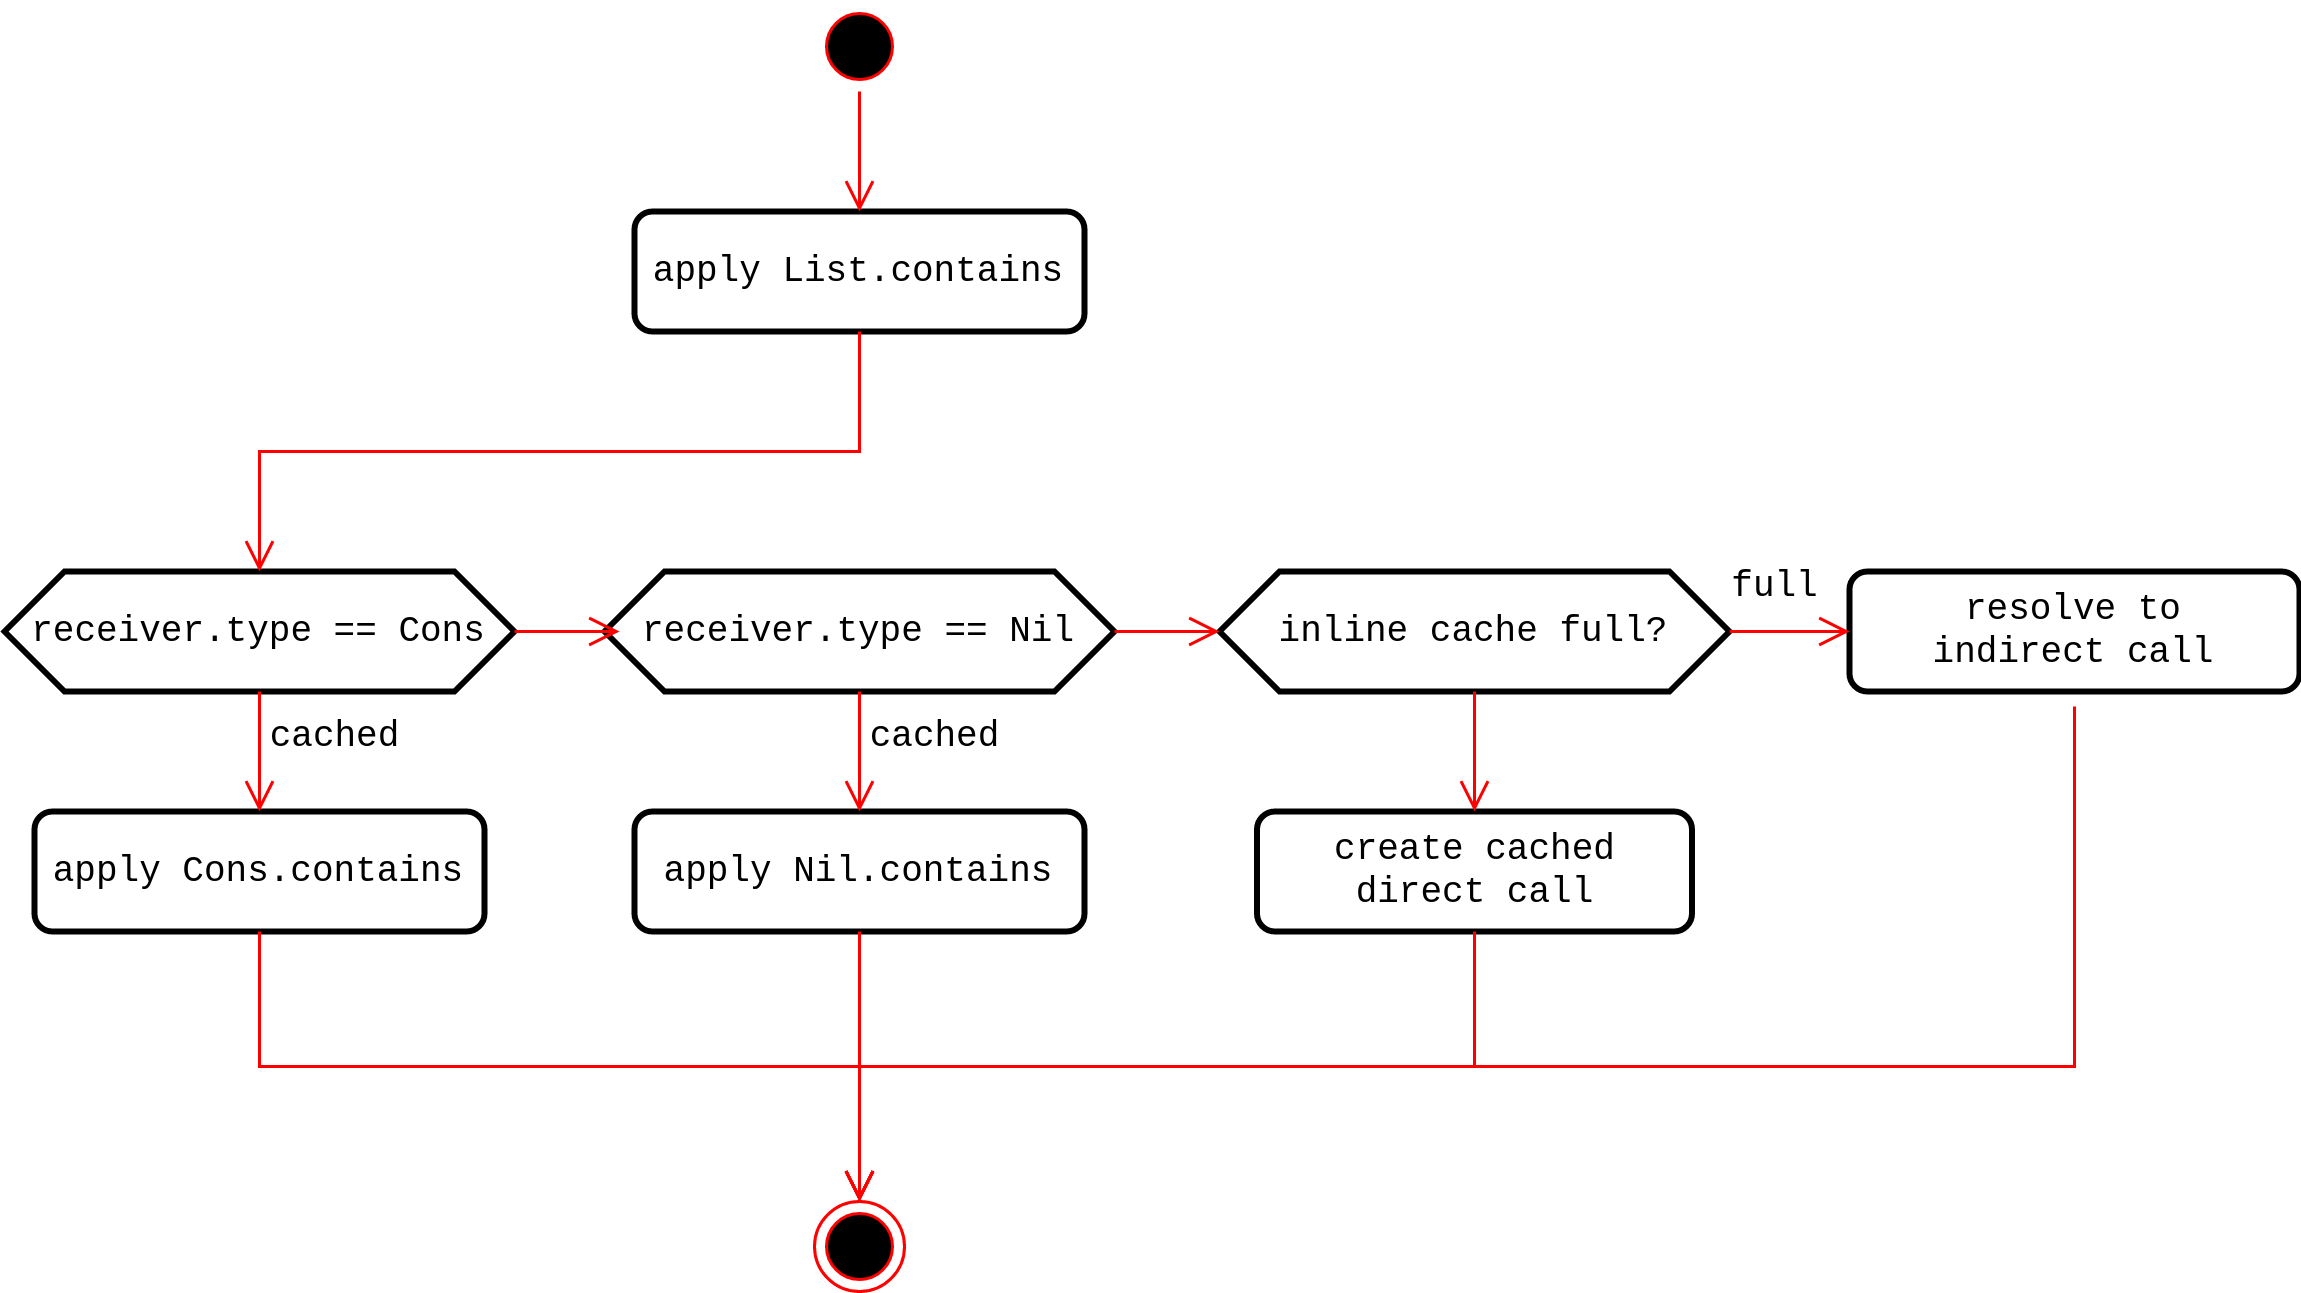
\includegraphics[width=0.6\textwidth]{figures/tastytruffle-pic-example.png}
	\caption{A possible polymorphic inline cache for a \scalainline{List.contains} callsite.}
	\label{example:poly-cache-call-node}
\end{figure}

Figure \ref{example:poly-cache-call-node} shows a data flow diagram of the application of a polymorphic inline cache to a call site of \scalainline{contains} when the receiver type is statically known to be \scalainline{List}. 
The diagram shown assumes that the call site has previously been called with a receiver where the dynamic type has been both \scalainline{Cons} and \scalainline{Nil}.
The \scalainline{ApplyNode} will first check if the type of receiver at the call site has the type \scalainline{Cons}; If the check passes then the cached direct call node is invoked and the call is complete.
It will then do the same for the type \scalainline{Nil}.
Otherwise, the type of the receiver has not been seen before and the call target is resolved virtually then cached for the next invocation at this call site.

When the polymorphic inline cache is applied to a monomorphic call site (where the type of the receiver does not change), it simplifies to a single element inline cache\cite{smalltalk:inline-caches}. 
Because the type of the receiver at the call site remains stable, the cache look up of the call target based on the type always succeeds and the call site never fallbacks to using an indirect call node.

\subsubsection*{Accessing Fields}

In our subset of TASTy, the \scalainline{Select} tree represents a read of a field of a \scalainline{ClassInstance}.
Notice in the resolution of the \scalainline{Apply} tree that an \scalainline{Apply} tree represents a method invocation when the applicator is a \scalainline{Select}.
Because functions are first-class objects in Scala, the TASTy tree for a method invocation is the access of a method as if it were a field then the application of the subsequent function value read to a list of arguments.
Since this case is handled previously when parsing the \scalainline{Apply} tree, a \scalainline{Select} tree always selects a value definition.

\begin{figure}[!htb]
	\begin{minted}{scala}
	@NodeChild("receiver")
	@NodeField("symbol", Symbol.class)
	abstract class ReadFieldNode extends TermNode {
		final val INLINE_CACHE_SIZE: Int = 3;
			
		@Specialization(guards = "instance.getShape == shape", limit = "INLINE_CACHE_SIZE")
		def cached(
			instance: ClassInstance,
			@Cached("instance.getShape") shape: ClassShape,
			@Cached("lookupField(shape)") field: Field
		): Object = field.getContents(instance)
			
		@Specialization(replaces = "cached")
		def virtual(instance: ClassInstance): Object = {
			val field = lookupField(instance.getShape)
			field.getContents(instance)
		}
	
		private def lookupField(shape: ClassShape): Field = shape.getField(symbol)
	}
	\end{minted}
	\caption{Pseudocode of field read node with a polymorphic inline cache.}
	\label{impl:field-read-node}
\end{figure}

Figure \ref{impl:field-read-node} gives a simplified implementation of a field read node.
Like the virtual dispatch of call targets, fields are resolved dynamically with the shape of a \scalainline{ClassInstance}.
We apply a polymorphic inline cache to the lookup of field properties to eliminate the performance overhead associated with this kind of virtual dispatch.

\subsubsection*{Accessing Locals and Globals}

\begin{figure}[!htb]
	\begin{minted}{scala}
	def parse(ident: Ident): TermNode = {
		if (ident.symbol.isObjectDef)
			new ReadGlobalNode(symbol)
		else 
			new ReadLocalNode(localOf(symbol))
	}
	\end{minted}
	\caption{Pseudocode to parse an \scalainline{Ident} tree.}
	\label{impl:parse-ident}
\end{figure}

The \scalainline{Ident} tree is a name that refers to either a local value or a global value.
Local values take the form of a local variable or a method parameter.
Global values refer to a top level \scalainline{object} definition.
We differentiate between a local and a global based on whether the symbol of the \scalainline{Ident} tree refers to an \scalainline{object} definition (shown in figure \ref{impl:parse-ident}).

\begin{figure}[!htb]
	\begin{minted}{scala}
	object Globals {
		val values: Map[Symbol, ClassInstance] = ???
	}
	
	class ReadGlobalNode(symbol: Symbol) extends TermNode {
		override def execute(frame: VirtualFrame): Object = Globals.values.get(symbol)
	}

	class ReadLocalNode(local: Local) extends TermNode {
		override def execute(frame: VirtualFrame): Object = frame.getObject(local.index)
	}
	\end{minted}
	\caption{Pseudocode of local and global value read nodes.}
	\label{impl:local-global-node}
\end{figure}

Figure \ref{impl:local-global-node} provides the implementations the \scalainline{ReadGlobalNode} and \scalainline{ReadLocalNode}.
In our interpreter, local variables and method parameters are uniformly represented by the frame slot abstraction.
During parsing, it is sufficient to maintain a mapping from symbols to a \scalainline{Local} to adequately resolve which local variable is read.
Truffle does not provide an abstraction for storing global values.
Instead, we retain a mapping of symbols to instances for all global object value definitions.
Recall from figure \ref{impl:top-level} that a top level value definition is registered.
When the symbol of an \scalainline{Ident} refers a \scalainline{object} definition, the value is resolved by using the symbol.

\subsubsection*{Mutating Values}

\begin{figure}[!htb]
	\begin{minted}{scala}
	def parseAssign(assign: Assign): TermNode = assign match {
		case Assign(select: Select, rhs) => 
			new WriteFieldNode(parse(select.qualifier), select.symbol, parse(rhs)) 
		case Assign(ident: Ident, rhs) =>
			new WriteLocalNode(localOf(ident.symbol), parse(rhs)) 
	}
	\end{minted}
	\caption{Pseudocode to parse an \scalainline{Assign} tree.}
	\label{impl:parse-assign}
\end{figure}

The \scalainline{Assign} tree has context-dependent semantics based on the structure of its left-hand side term.
Figure \ref{impl:parse-assign} contains the simplified logic to resolve \scalainline{Assign} trees into the appropriate term nodes.
If the left hand side term is a \scalainline{Select} tree, the current tree mutates the field of a \scalainline{ClassInstance}.
Otherwise, the left hand side is an \scalainline{Ident} which refers to local variable in the frame.
We differentiate between which node to generate based on the type of the tree seen on the left hand side.
The \scalainline{WriteFieldNode} and \scalainline{WriteLocalNode} mirror their read node counterparts but instead of reading from their respective locations, they update the value at their locations instead.

\subsubsection*{Conditionals}

\begin{figure}[!htb]
	\begin{minted}{scala}
	def parseIf(i: If): IfNode = new IfNode(parse(i.cond), parse(i.thenp), parse(i.elsep))
		
	class IfNode(@Child cond: TermNode, @Child t: TermNode, @Child f: TermNode) {
		val cp = ConditionProfile.create();
			
		override def execute(frame: VirtualFrame): Object = {
			if (cp.profile(cond.executeBoolean(frame)))
				t.execute(frame)
			else 
				f.execute(frame)		
		}
	}
	\end{minted}
	\caption{Pseudocode for parsing an \scalainline{If} into an \scalainline{IfNode}}
	\label{impl:if}
\end{figure}

The implementation of conditional control flow in our interpreter is quite simple.
Two execution paths exists for the two possible results from evaluating the condition term; The path taken depends on the boolean after evaluation.
An \scalainline{IfNode} is derived from an \scalainline{If} tree (given in figure \ref{impl:if}), which allows for divergence in program control flow.
The implementation of the TastyTruffle IR mirrors the semantics given by its original TASTy tree.
In order to take advantage of conditional speculative optimization, we add a \javainline{ConditionProfile} onto the result of the condition term.
A condition profile records the likelihood that a branch is either true or false.
Graal then speculatively optimizes the frequently true or false branches of an \scalainline{IfNode} using its condition profile.

\subsubsection*{Loops}

In our subset of TASTy, the \scalainline{While} tree is the only looping construct.
The control flow of the \scalainline{While} tree is quite simple; the body term is executed as long as the condition term holds at the beginning of every iteration.
Truffle provides the \scalainline{LoopNode} abstraction for implementations of guest language loop structures.
The loop node abstraction allows guest languages to take advantage of \textit{On-Stack Replacement}\cite{osr}.
On-stack replacement is a technique which switches control of part of a program running in the interpreter to compiled code while that part is executing.

\begin{figure}[!htb]
	\begin{minted}{scala}
	def parseWhile(tree: While): WhileNode = new WhileNode(parse(tree.cond), parse(tree.body))	
		
	class WhileNode(@Child cond: TermNode, @Child body: TermNode) extends TermNode {
		
		@Child val loopNode: LoopNode = 
			Truffle.getRuntime.createLoopNode(new WhileRepeatingNode(cond, body))
		
		override def execute(frame: VirtualFrame): Object = {
			loopNode.execute(frame)
			()
		}
		
		class WhileRepeatingNode(
			@Child cond: TermNode, 
			@Child body: TermNode
		) extends Node with RepeatingNode {
			val cp = ConditionProfile.create()
			
			override def executeRepeating(frame: VirtualFrame): Boolean = 
				if (cp.profile(cond.executeBoolean(frame))) {
					body.execute(frame)
					true 
				} else false 
				
		}
	}
	\end{minted}
	\caption{Pseudocode for a \scalainline{WhileNode}}
	\label{impl:while}
\end{figure}

So far in this thesis, the root node has been the primary compilation unit in Graal.
Root nodes profile their invocation count and get JIT compiled when they've been invoked frequently.
However, loop constructs which are executed for many iterations also justify JIT compilation.
The loop node is an additional type of JIT compilation unit which Graal can compile.
A key difference between loop nodes and root nodes is when their compiled equivalents are utilized.
While compiled root nodes are used in subsequent invocations of their call targets after they are JIT compiled, compiled loop nodes are used in the next iteration after they are JIT compiled.
As on-stack replacement is not a central focus of this thesis, we will only discuss it briefly because loop nodes are the recommended abstraction for guest languages to implement loop structures in Truffle.

Figure \ref{impl:while} contains the implementation of a \scalainline{WhileNode} and its derivation from a \scalainline{While} tree.
Like our implementation of the \scalainline{IfNode}, we add a condition profile onto the node which evaluates the termination condition inside \scalainline{WhileRepeatingNode}.
Truffle will automatically instrument the \scalainline{WhileNode}.
After sufficient iterations of the \scalainline{WhileRepeatingNode}, the repeating node is compiled and the next iteration of the \scalainline{WhileNode} will use the compiled repeating node.

\subsubsection*{Blocks}

\begin{figure}[!htb]
	\begin{minted}{scala}
	def parseBlock(block: Block): BlockNode = {
		val desc = getParentFrameDescriptor(block)
			
		val terms = block.statements map {
			case vdef: ValDef => generateBlockLocal(desc, vdef)
			case term => term 
		}
			
		new BlockNode(terms, parse(block.expr))
	}
		
	def generateBlockLocal(desc: FrameDescriptor, vdef: ValDef): TermNode = {
		val local = generateLocal(vdef)
		new WriteLocalNode(local, parse(vdef.rhs))
	}	
	\end{minted}
	\caption{Pseudocode for parsing \scalainline{Block} into \scalainline{BlockNode}}
	\label{impl:parse-block}
\end{figure}

In this section, we cover the translation of the \scalainline{Block} tree to its TastyTruffle IR equivalent.
The \scalainline{Block} is unique among term trees as it describes data as well as code.
In our subset of TASTy, this means that a block may contain declarations of local variables as well as executable terms.
Figure \ref{impl:parse-block} provides an overview on the transformations necessary to convert a \scalainline{Block} tree into \scalainline{BlockNode}.
We divide the discussion of blocks into the resolution of local variables when encountering a \scalainline{ValDef} tree and the execution of all other trees.

Local variables are variables which are bound to a \textit{scope}. 
A scope represents the lifetime in which a variable can refer to an value. 
Similarly, uses of variables are only valid when used under the appropriate scope. 
Local variables and their use sites are represented in intermediate representations through a myriad of methods. 
In abstract syntax trees, local variables and their used are represented as nodes \textit{dominated} by their scopes (which are themselves nodes). 
In our subset of TASTy, a \scalainline{ValDef} dominated by a \scalainline{Block} represents a local variable.
When a \scalainline{ValDef} tree is present in this context, the right hand side of the value definition will be non-empty.

\begin{figure}[!htb]
	\begin{minted}{scala}
	class BlockNode(stats: Array[TermNode], last: TermNode) extends TermNode {
		@ExplodeLoop
		override def execute(frame: VirtualFrame): Object = {
			for (stat <- stats) 
				stat.execute(frame)
					
			last.execute(frame)
		}
	}
	\end{minted}
	\caption{Pseudocode of the \scalainline{BlockNode}}
	\label{impl:block-node}
\end{figure}

Because terms always return a value, the \scalainline{Block} tree must follow the same semantics.
Figure \ref{impl:block-node} gives the pseudocode for our implementation of a \scalainline{BlockNode}.
The \javainline{@ExplodeLoop} is a Truffle DSL directive which guides Graal to unroll\cite{loop-unrolling} the loop for execution of each child node.
Unrolled loops simplify partial evaluation as each iteration of the loop is treated as an individual statement and thus they reveal constant values which are easier to partial evaluate.
As the number of children in a \scalainline{BlockNode} is known before execution, it makes sense to unroll this loop in order to simplify optimization.

\subsubsection*{Returns}

\begin{figure}[!htb]
	\begin{minted}{scala}
	class ReturnException(result: Object) extends ControlFlowException
	
	class ReturnNode(@Child term: TermNode) extends TermNode {
		override def execute(frame: VirtualFrame): Object = { 
			val result = term.execute(frame)
			throw new ReturnException(result)
		}
	}
	\end{minted}
	\caption{Pseudocode of \scalainline{ReturnException} and \scalainline{ReturnNode}}
	\label{impl:return}
\end{figure}

A \scalainline{Return} trees ends the execution of the current methods and passes a value back to the caller.
The semantics of returning control flow in Truffle is implemented as a program \textit{exception}.
Recall in figure \ref{impl:defdefnode} that a body of a \scalainline{DefDefNode} is execute and a \scalainline{ReturnException} is possibly caught.
The implementation of the \scalainline{ReturnException} and \scalainline{ReturnNode} is given in figure \ref{impl:return}.
The \scalainline{ReturnException} is a subclass of the special \javainline{ControlFlowException}. 
A return exception is thrown with the return value evaluated from a return node.
The exception is then caught by the executing \scalainline{DefDefNode}, where the return value is passed back to the caller as the result. 

 \subsubsection*{Putting it All Together}

\begin{figure}[!htb]
	\begin{minted}{scala}
	Block(
		List(
			ValDef("these", _, This),			
			While(
				Apply(Select(Ident("these"), "empty"), "!", List.empty),
				If(
					Apply(Select(Select(Ident("these"), "head")), "==", List(Ident("elem")))
					Return(Constant(true)),
					Assign(Ident("these"), Select(Ident("these"), "tail"))
				)	
			)   
		),
		Constant(false)
	)
	\end{minted}
	\caption{TASTy of \scalainline{Cons.contains}}
	\label{tasty:list-contains}
\end{figure}

In this section, we summarize all the tree transformations introduced for the monomorphic variant of our interpreter.
Figure \ref{tasty:list-contains} is the structure of the \scalainline{Cons.contains} method in TASTy.
We have omitted the type tree which has been declared inside the local variable definition.
We use the \scalainline{Cons.contains} method as an example to summarize the transformations described in this section.

\begin{figure}[!htb]
	\begin{minted}{scala}
	BlockNode(
		Array(
			WriteLocalNode("these", ReadLocalNode("this")),
			WhileNode(
				UnaryOpNode("!", ApplyNode("these", "List.isEmpty[0]()", Array.empty)),
				IfNode(
					ApplyNode(
						FieldReadNode(ReadLocalNode("these"), "head"), 
						"Any.==[0]()", 
						ReadLocalNode("elem")
					),
					ReturnNode(ConstantNode(true)),
					WriteLocalNode("these", ReadFieldNode(ReadLocalNode("these"), "tail")),	
				)   
			)
		),
		ConstantNode(false)
	)
	\end{minted}
	\caption{\scalainline{Cons.contains} as a Truffle AST}
	\label{example:truffle-list-contains}
\end{figure}

Figure \ref{example:truffle-list-contains} is the Truffle equivalent AST of \scalainline{Cons.contains}.
We use simple strings to represent symbols and method signatures in order to avoid unnecessary detail in the example.
Notice that many TASTy nodes have an equivalent TastyTruffle IR which closely mirrors their structure.
However, other TASTy nodes must be simplified to a representation more suitable for runtime.
In particular, \scalainline{ValDef} trees are eliminated and replaced by an initializer node which assumes that the frame slot for the local variable definition was added during parsing.
In the second half of this chapter we will describe the challenges of using these trees in the presence of parametric polymorphism and their associated performance overhead.

\section{The Polymorphic Interpreter}
\label{implementation:specialization}

\begin{figure}[!htb]
	\begin{minted}{scala}
	abstract class TypeNode extends Term {
		override final def execute(frame: VirtualFrame): Object = resolveType(frame)
		def resolveType(frame: VirtualFrame): Type 
	}
	\end{minted}
	\caption{An abstract type node.}
	\label{impl:type-node}
\end{figure}

In this section, we extend our interpreter to support the execution of polymorphic trees.
To that end, we introduce the notion of \textit{reified} type nodes.
In essence, to implement specialization of polymorphic classes and methods, we make types a \textit{first-class} value.
Like the \scalainline{TermNode} represents the \scalainline{Term} tree node from TASTy, the \scalainline{TypeNode} represents the \scalainline{Type} from TASTy but instead of producing a value from evaluation, it produces a \textit{type}
To better illustrate this concept, figure \ref{impl:type-node} contains the implementation of the node superclass which evaluates to a type and not a value.

Because the underlying type of a type parameter is only known during runtime, introducing types during execution allows data layouts to be determined at runtime.
The type node is the abstraction we use to encapsulate this concept.
The principal idea behind the type node is to allow for the resolution of types during runtime.
Retaining the ability to resolve types during runtime avoids the pitfalls of type erasure.
Using the newly available type information during runtime, The layout of data can be specialized based on the types seen.
In the following subsections, we will focus on specific instances of boxing using Graal IR of compiled code executed using the monomorphic interpreter.
Then we introduce subclasses of the \scalainline{TypeNode} and show how reified types can be utilized to specialize the data structures from monomorphic interpreter.

\subsection{Specializing Methods}

\begin{figure}[!htb]
	\begin{minted}{scala}
	class DefDefTemplate(
		desc:    FrameDescriptor
		tparams: Int, 
		vparams: List[ValDef], 
		rhs:     Term
	) extends RootNode {
		def execute(frame: VirtualFrame): Object = ???
		
		def specialize(types: Array[Type]): DefDefNode = {
			val desc = new FrameDescriptor
			
			val types = resolveTypeParameters
			val parameters = self :: vparams.map {
				case vdef: ValDef => createParameter(types, vdef, desc)
			}
				
			val body = parse(rhs)
			new DefDefNode(desc, parameters, body)
		}
	}
	\end{minted}
\end{figure}

Polymorphic methods in Scala can be polymorphic under class type parameters, method type parameters, or both. 
In this section, we will focus only on the specialization of methods which are polymorphic under their own type parameters.
We defer the discussion of the specialization of class-polymorphic methods until the next section.
We will introduce the concept of a \textit{template}; Templates retain sufficient information about the data layout of a definition in TASTy to generate their runtime equivalent representations dynamically.
In the case of a polymorphic method, a \scalainline{DefDefTemplate} replaces a \scalainline{DefDefNode}.

\begin{figure}[!htb]
	\begin{minted}{scala}
	def createParameter(types: Array[Type], defn: ValDef | TypeDef, desc: FrameDescriptor): LocalVal = 
		defn match {
			case tdef: TypeDef => 
				val kind = FrameSlotKind.Object
				val slot = desc.addSlot(kind)
				LocalVal(slot, ReifiedType)
			case vdef: ValDef => 
				val idx = indexOf(vdef.tpt.tpe)
				val tpe  = if (idx != -1) types(idx) else vdef.tpt.tpe
				val kind = getFrameSlotKind(tpe)
				val slot = desc.addSlot(kind)
				LocalVal(slot, tpe)
		}
	\end{minted}
\end{figure}

The \scalainline{DefDefTemplate} itself can also be invoked.
Because the type of a method specialization is derived from one of its call sites, the specialized root node must be created \textit{after} invocation.
The execution semantics of a \scalainline{DefDefTemplate} should select the appropriate specialization and forward the original invocation arguments to that specialization.
We defer the complete explanation on the invocation and dynamic specialization mechanism after the explanation of how the data layout of a root node changes from specialization.

\begin{figure}[!htb]
	\begin{minted}{scala}
	def parseDefDef(ddef: DefDef): DefDefNode | DefDefTemplate = {		
		val tparams = ddef.params.filter(_.isInstanceOf[TypeDef]).length
		val isPolymorphic = hasPolymorphicTerms(ddef.rhs) // polymorphic from class or method type parameters
		if (tparams == 0 && !isPolymorphic)
			createDefDefNode(ddef)
		else {
			val vparams = ddef.filter(_.isInstanceOf[ValDef])
			new DefDefTemplate(desc, tparams, vparams, ddef.rhs)
		}
	}

	def createDefDefNode(ddef: DefDef): DefDefNode // a monomorphic DefDef
		
	...
	\end{minted}
	\caption{Pseudocode for parsing \scalainline{DefDef} into \scalainline{DefDefNode}}

\end{figure}

The \scalainline{DefDefTemplate} stores the value definitions and polymorphic terms from its \scalainline{DefDef}.

\subsubsection*{Polymorphic Method Parameters}

\begin{figure}[!htb]
	\centering
	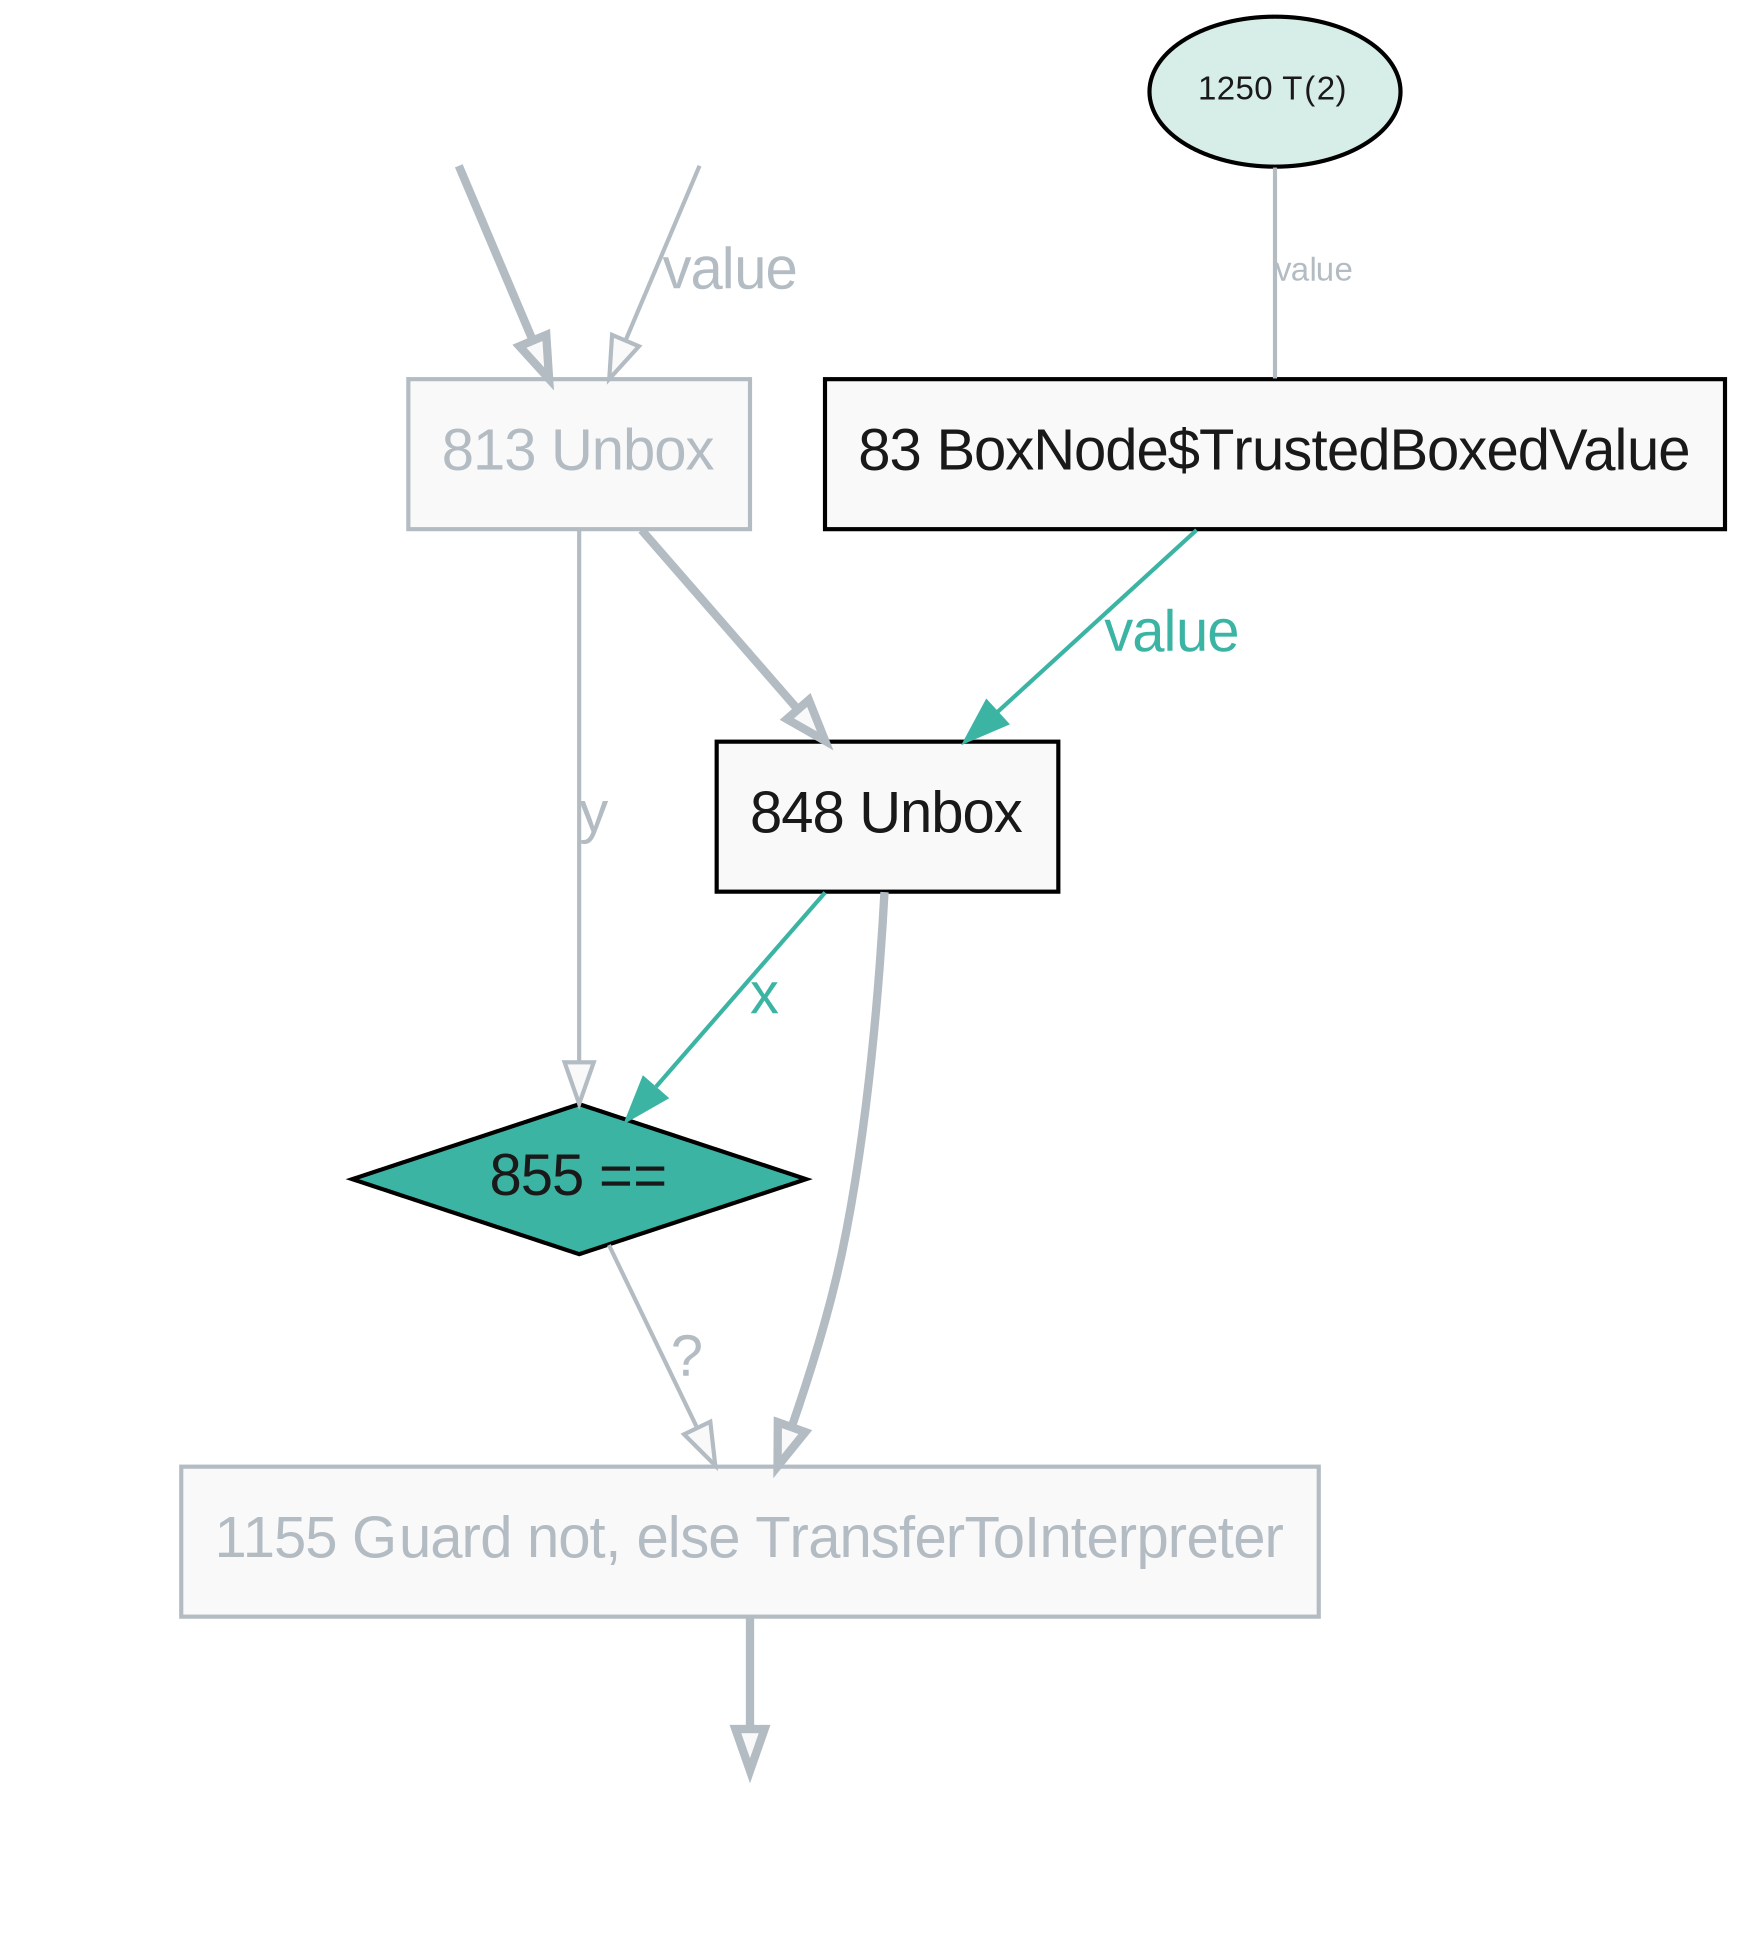
\includegraphics[width=0.4\textwidth]{figures/dot/List.contains.boxed-param-read.TruffleTier.png}
	\caption{Graal IR with speculative unboxing of \scalainline{elem} based on a type profile of its frame slot in \scalainline{List.contains}}
	\label{graalir:cons-contains-param-read}
\end{figure}

Truffle conveniently profiles the types of frame arguments to speculatively eliminate the unboxing of boxed values when reading frame values (including arguments).
Figure \ref{graalir:cons-contains-param-read} is an example of such a speculative optimization.
This speculative optimization relies on a \javainline{TrustedBoxedValue} to unbox the primitive.
A \javainline{TrustedBoxedValue} represents injected information from an external source.
In this particular case, it is known by the compiler that boxed instance comes from a cache; Unique \javainline{int} values may be mapped to a unique \javainline{Integer} instance in the Java runtime, which eliminates unnecessary boxed object creation.
The unbox operation in node $848$ will be `floated' up the graph such that all subsequent dominated by the read of a boxed frame value has no autoboxing.

In contrast, write operations of polymorphic frame values cannot be speculatively eliminated. 
Because Truffle does not specialize data layouts, i.e. frames are determined by their descriptors, which in turn are determined by the guest language implementation, frame writes of polymorphic values will always have to be boxed.
This is the main advantage when specializing the frame descriptor of a root node.
Code that has polymorphic code which reads and writes to a frame frequently will no longer have to unbox, compute primitive operations on unboxed values, then box those values back into their respective slots.
As our running example does not make use of this particular pattern of autoboxing, we will take this opportunity to showcase an instance of a polymorphic value read operation that Truffle is unable to speculatively optimize without specialization.

In both Scala and the JVM, arrays of primitive types are invariant with respect to the $\top$ (the universal supertype) type, \scalainline{Any} and \javainline{Object} in Scala and Java respectively.
That is to say, the type \scalainline{Array[Int]} is neither a subtype or supertype of the type \scalainline{Array[Any]}.
On the other hand, the type \scalainline{AnyRef} is covariant to the \scalainline{Array[Any]} type.
This contradiction in the presence of code which creates or operates on polymorphic arrays requires runtime bridge methods in order to appear seamless to the programmer.
These bridge methods combined with the nature of Scala's type system obscure opportunities for speculative optimizations.

\subsubsection*{Case Study: A List Constructor}

\begin{figure}[!htb]
	\begin{minted}{scala}
	object List {
		def apply[T](array: Array[T]): List[T] = {
			var i = array.length - 1
			var these: List[T] = Nil
			while (i >= 0) {
				these = new Cons[T](array(i), these)
				i -= 1
			}
			these
		}	
	}
	\end{minted}
	\caption{An alternate static constructor that converts an \scalainline{Array[T]} to a \scalainline{List[T]}}
	\label{impl:list-alt-constructor}
\end{figure}

To showcase an instance of when polymorphic array code must be bridged, we define an alternate constructor for a \scalainline{List[T]} to use an as example.
Figure \ref{impl:list-alt-constructor} gives a constructor that creates a polymorphic list from a polymorphic array.
We focus on the term \scalainline{array.length} which computes the length for a polymorphic array on line $3$.
When the Typer detects an array operation on a polymorphic array value, it automatically inserts the array runtime bridge method that is responsible for handling the operation.
For example, line $3$ after the Typer would be transformed into \scalainline{var i = array_length(array) - 1}.
We give the implementation of \scalainline{array_apply} in figure \ref{impl:array-length}.

\begin{figure}[!htb]
	\begin{minted}{scala}
	def array_length(array: AnyRef): Int = {
		if (array.isInstanceOf[Array[AnyRef]])       array.asInstanceOf[Array[AnyRef]].length
		else if (array.isInstanceOf[Array[Int]])     array.asInstanceOf[Array[Int]].length
		else if (array.isInstanceOf[Array[Double]])  array.asInstanceOf[Array[Double]].length
		else if (array.isInstanceOf[Array[Long]])    array.asInstanceOf[Array[Long]].length
		else if (array.isInstanceOf[Array[Float]])   array.asInstanceOf[Array[Float]].length
		else if (array.isInstanceOf[Array[Char]])    array.asInstanceOf[Array[Char]].length
		else if (array.isInstanceOf[Array[Byte]])    array.asInstanceOf[Array[Byte]].length
		else if (array.isInstanceOf[Array[Short]])   array.asInstanceOf[Array[Short]].length
		else if (array.isInstanceOf[Array[Boolean]]) array.asInstanceOf[Array[Boolean]].length
		else throw new NullPointerException
	}
	\end{minted}
	\caption{Implementation of \scalainline{array_length}}
	\label{impl:array-length}
\end{figure}

Notice the type of the argument in \scalainline{array_length} is \scalainline{AnyRef}; Because the types of primitive arrays and reference arrays are invariant, the direct supertype is \scalainline{AnyRef}.
To compute the length for a polymorphic, \scalainline{array_length} switch over every similar but unrelated array type.
In the body of every type check condition, the argument must be be cast to the appropriate array type after the type check succeeds before the length is finally computed.
We will examine how this code looks in the context of our alternate constructor after JIT compilation in Graal IR.

\begin{figure}
	\centering
	\includegraphics[width=\textwidth]{figures/dot/List.apply.boxed.array_length.png}
	\caption{Graal IR of \scalainline{array_length} in the context of \scalainline{List.apply[T](array: Array[T])}}
	\label{graalir:list-apply-boxed-array-length}
\end{figure}

Figure \ref{graalir:list-apply-boxed-array-length} contains the Graal IR of \scalainline{array_length} inlined into \scalainline{List.apply[T]}. 
Notice that the \scalainline{instanceof} type checks nodes (white) that are succeeded by an \javainline{ArrayLength} node (red) for each of the branches in \scalainline{array_length}.
The numerous consecutive conditional expressions complicate the control flow analysis in JIT compilation.
These conditional add unnecessary branching and burdens JIT compilation when the type of a specialized array should be known.
We introduce a method to vastly simplify the Graal IR of such instances of array bridge methods when specialized methods would have type-specific information to augment JIT compilation.

\begin{figure}[!htb]
	\begin{minted}{scala}
	import CompilerDirectives.castExact
	def copyArgumentsToFrame(frame: VirtualFrame): Unit = 
		for ((param, arg) <- params zip frame.getArguments) 
			param.tpe match {
				case Int =>
					frame.setInt(param.slot, arg.asInstanceOf[Int])
				...
				case Double =>
					frame.setDouble(param.slot, arg.asInstanceOf[Double])	
				case tpe: Array[AnyRef] | tpe: Array[Int] | ... | tpe: Array[Double] =>
					frame.setObject(param.slot, castExact(arg, getClass(tpe)))
				case _ =>
					frame.setObject(param.slot, arg)
			}
	\end{minted}
	\caption{Pseudocode for \scalainline{DefDefNode} and \scalainline{Parameter}}
	\label{impl:specialized-copy-arguments}
\end{figure}

In order to accomplish this, we extend the way that frame arguments are copied into the frame from figure \ref{impl:defdefnode}.
Because a parameter now retains its type instead of a frame slot kind, we introduce a special operation when copying arguments that are arrays. 
The \javainline{castExact} directive is a type narrowing operation that hints to Graal that a value is an instance of a type.
We will examine how the insertion of this directive for array types simplify the layout of Graal IR graphs.

\begin{figure}[!htb]
	\centering
	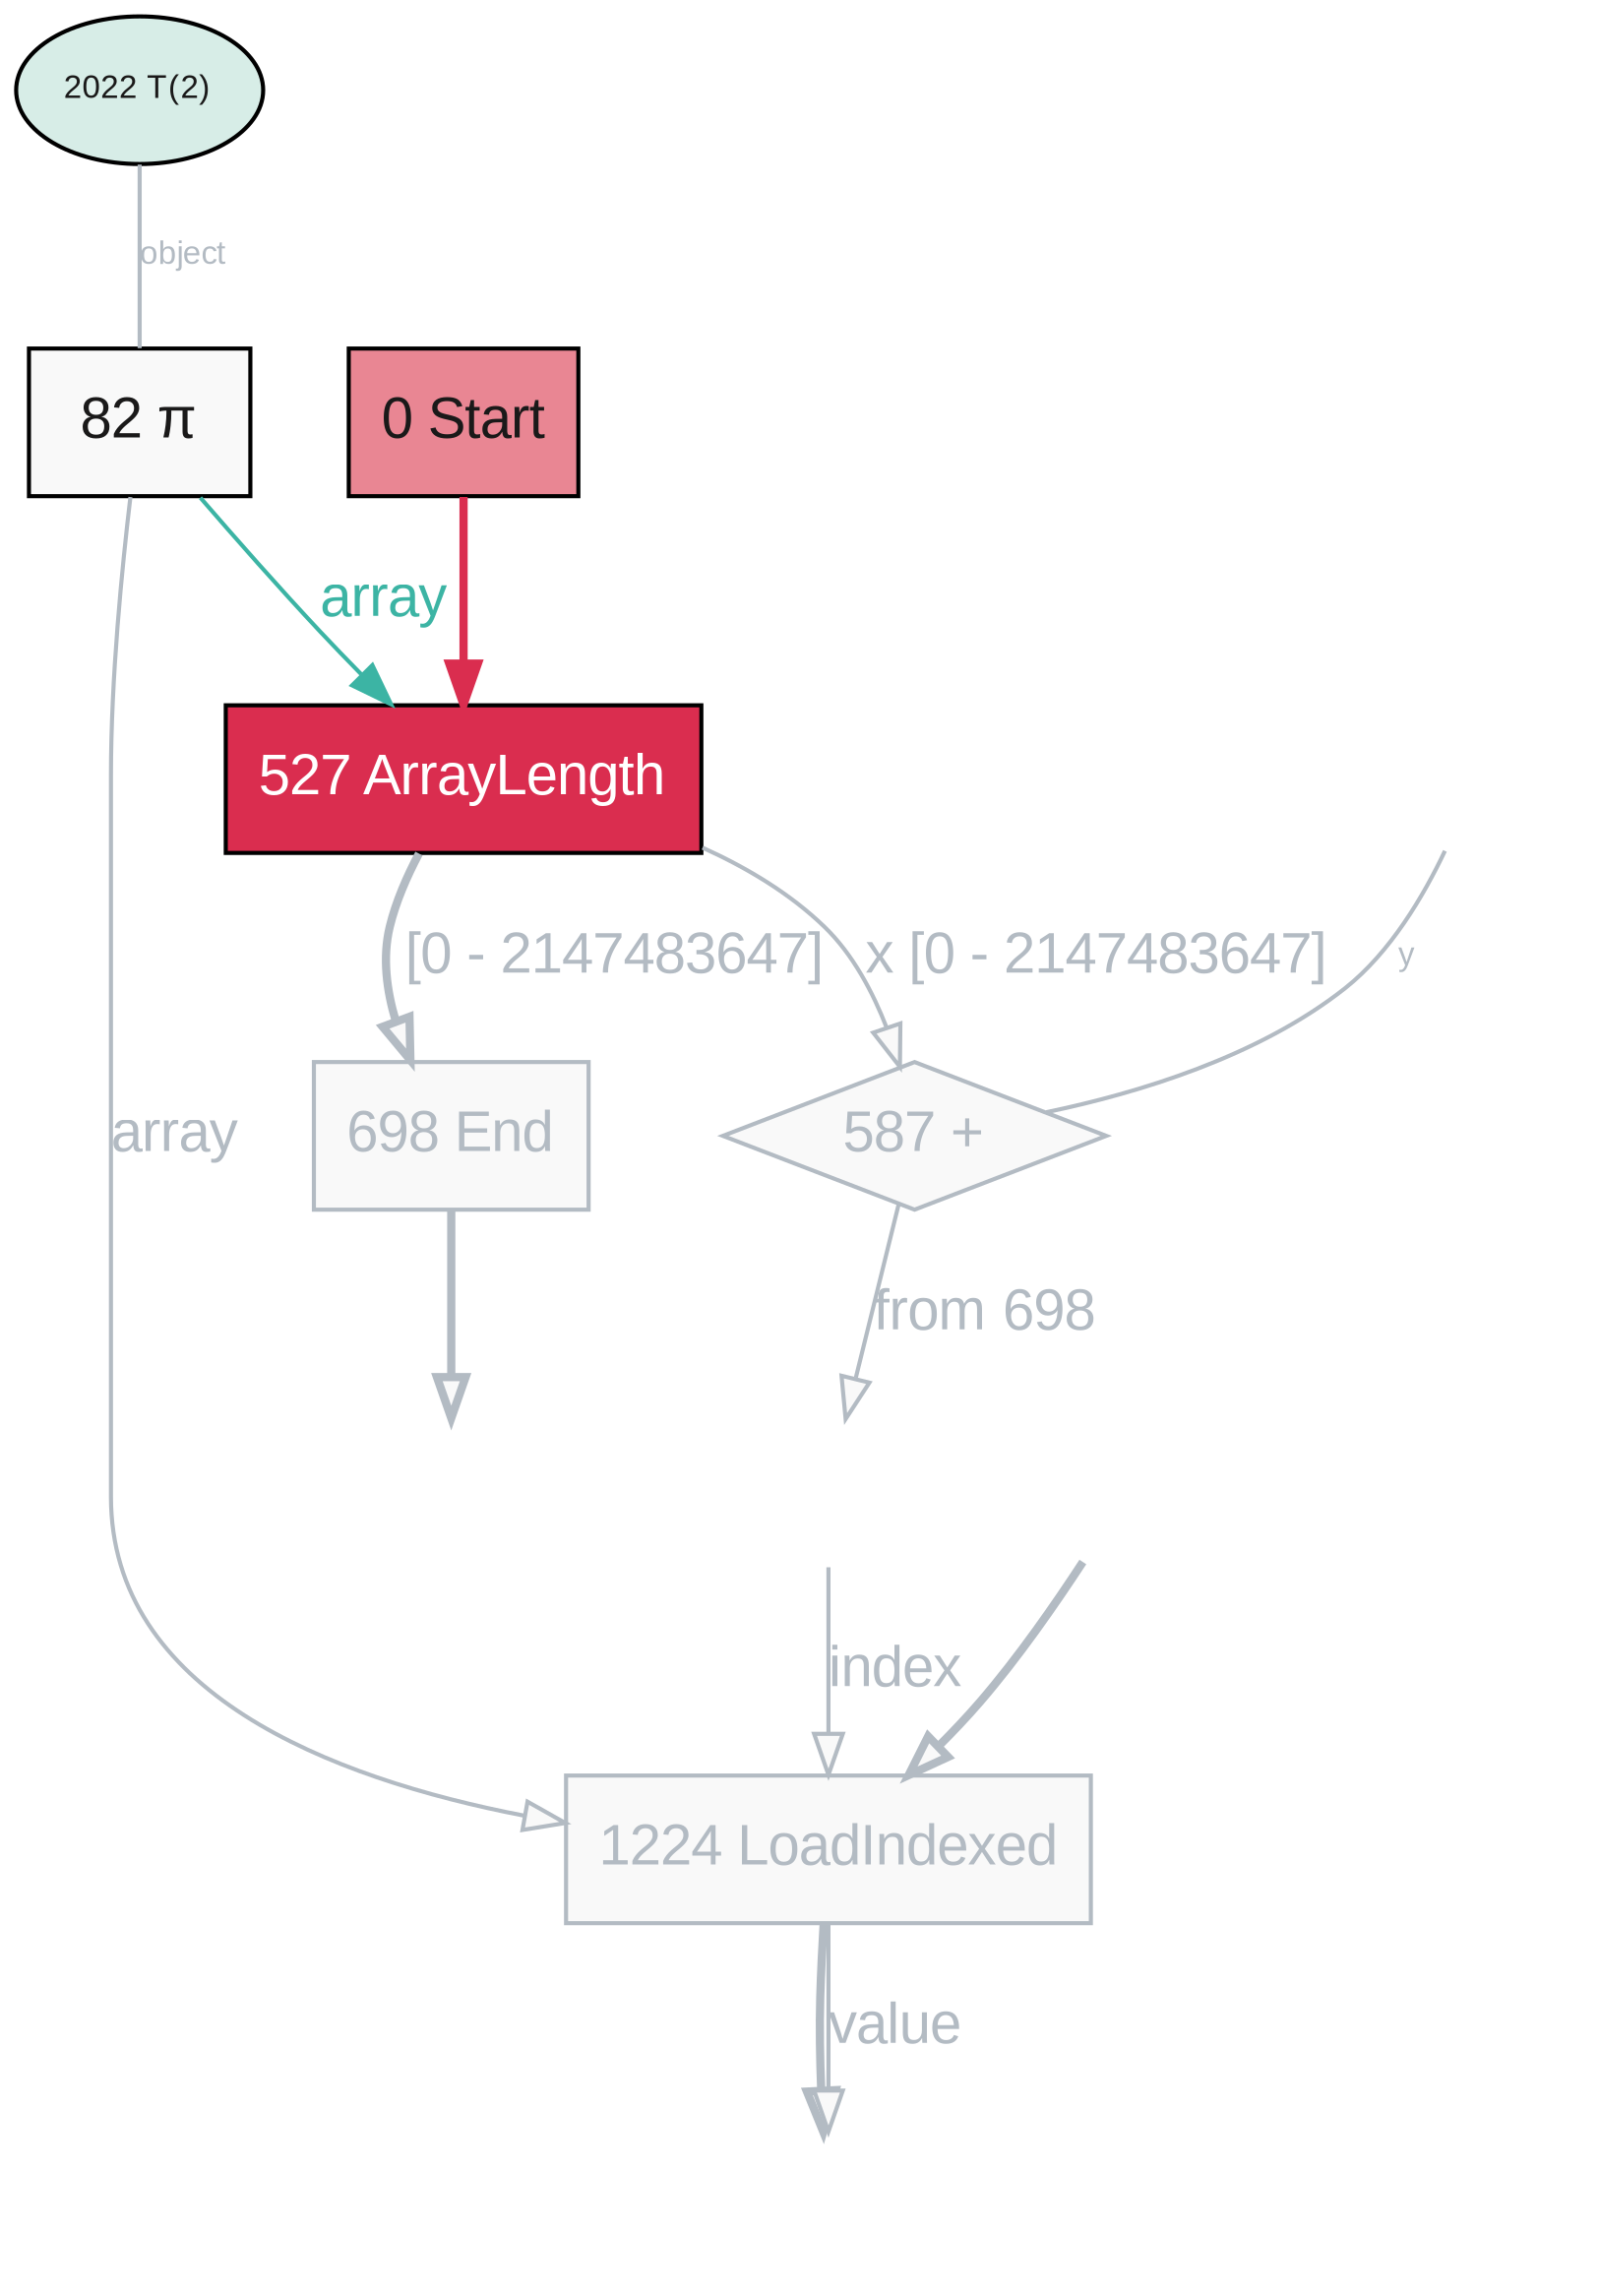
\includegraphics[width=0.3\textwidth]{figures/dot/List.apply.specialized.array_length.png}
	\caption{Graal IR of \scalainline{array_length} in the context of \scalainline{List.apply[T](array: Array[T])} augmented with a $\pi$ node}
	\label{graalir:list-apply-specialized-array-length}
\end{figure}

Figure \ref{graalir:list-apply-specialized-array-length} contains the simplified Graal IR of \scalainline{array_length} inlined into \scalainline{List.apply[T]}.
Notice that there is a single \javainline{ArrayLength} node that is dominated by a $\pi$ node.
A $\pi$ node\cite{abdc:pi-nodes} enforce a bound on value.
In the case of Graal, a $\pi$ node enforces bound on the type of a value.
More specifically in our example, the $\pi$ node narrows the type of the 2nd parameter of \scalainline{List.apply[T]} to a monomorphic array type.
When the type of the parameter is narrowed, the type checks that enforce array types from figure \ref{graalir:list-apply-boxed-array-length} are eliminated because the type is now known.

This method does not consider polymorphic scenarios where an array of boxed primitives are used interchangeably with an array of primitives.
Such scenarios would require the insertion of additional autoboxing nodes or an intraprocedural transformation where boxed arrays are converted to primitive arrays.
While these solutions are possible in the context of Truffle, we consider these kinds of scenarios out of the scope of this thesis.

\subsubsection*{Invoking Polymorphic Methods}

\begin{figure}[!htb]
	\begin{minted}{scala}
	def parseApply(apply: Apply): ApplyNode = {
		val signature = apply.symbol.signature
		apply match {
			case Apply(Select(qualfier, _), arguments) => ... // monomorphic trees
			case Apply(TypeApply(Select(qualifier, _), targs), args) =>
				new ApplyNode(signature, parse(qualifier), (targs ++ args).map(parse))
		}
	}
	\end{minted}
	\caption{Extension to parsing a polymorphic \scalainline{Apply} tree.}
	\label{impl:parse-typeapply}
\end{figure}

So far we have shown how to create a specialized method, but not when to create one.
For this demonstration, we will show one of the natural benefits of executing TASTy (and other high level intermediate representations).
A polymorphic method invocation in TASTy is always an \scalainline{Apply} tree node where the qualifier is a \scalainline{TypeApply}.
The \scalainline{TypeApply} tree node represents a \textit{type application}.
Without delving into great detail, a type application is the process of producing a monomorphic method from a polymorphic method by matching type parameters to type arguments.
Analogous to normal applications which accept values as arguments and produces values as results, type applications accept types as arguments and produce types as a result.
With this in mind, \scalainline{TypeApply} nodes are a naturally suitable site to invoke and create specializations for methods.

Figure \ref{impl:parse-typeapply} extends the transformation of \scalainline{Apply} tree nodes to include polymorphic applications.
The application of a polymorphic method follows the same semantics as the application of a monomorphic method.
The actual specialization of the frame layout occurs inside the template that a polymorphic \scalainline{ApplyNode} invokes.
This allows the invocation of polymorphic methods even in the presence of dynamic dispatch.
In the next section, we will describe additional machinery that is added \textit{after} a polymorphic inline cache has resolved virtual dispatch to handle type application and how to make such mechanisms amenable to partial evaluation.

\subsubsection*{Typed Dispatch Chains}

\begin{figure}[!htb]
	\begin{minted}{scala}
	class DefDefTemplate(...) extends RootNode(...) { 
			
		@CompilerDirectives.CompilationFinal
		val specializations: Array[(Array[Type], DirectCallNode)] = Array.empty
			
		def execute(frame: VirtualFrame): Object = {
			val typeArguments = resolveArguments
			dispatchCached(frame, types)
		}
			
		@ExplodeLoop
		def dispatchCached(frame: VirtualFrame, typeArguments: Array[Type]): Object = {
			for ((typeSignature, specialization) <- specializations)
				if (typeSignature == typeArguments)
					return specialization.call(frame.getArguments)
			CompilerDirectives.transferToInterpreterAndInvalidate()
			dispatchNew(frame, typeArguments)
		}
		
		def dispatchNew(frame: VirtualFrame, typeArguments: Array[Type]): Object = {
			val specialization = specialize(typeArguments)
			val callNode = DirectCallNode.create(specialization)
			specializations += (typeArguments -> callNode)
			callNode.call(frame.getArguments)
		}
		
		...
	}
	\end{minted}
	\caption{Pseudocode for typed dispatch inside a \scalainline{DefDefTemplate}.}
	\label{impl:defdeftemplate-execute}
\end{figure}

Dispatch chains\cite{trufflyruby:specialization} are multi-layered inline caches.
We introduce the notion of \textit{typed dispatch chains}.
Typed dispatch chains integrate the semantics of type applications onto the execution mechanism of a root node.
Figure \ref{impl:defdeftemplate-execute} contains the simplified implementation of the execution semantics in a \scalainline{DefDefTemplate}.

Specializations of polymorphic methods are created on demand then cached based on their type signatures.
One particular challenge of making caching mechanism fold away in partial evaluation is that the cache must be a \textit{compilation constant}.
Truffle provides the \javainline{CompilationFinal} directive which indicates that a value which may not be a constant in the guest language implementation \textit{will} be a constant when being partially evaluated.
Type arguments at type application sites are always stable, i.e. their respective type nodes evaluate to the same type, the look up of the specialized call node should have no overhead when JIT compiled with aid of partial evaluation. 
To make this possible, we exploit a simple array of type signature and specialized call node pairs.
When the loop for looking up a cache entry in the array is unrolled during partial evaluation (directed by \javainline{ExplodeLoop}), the loop is transformed into a block of conditional expressions for each cache entry.
This unrolled loop combined with the injected knowledge that type argument values are compilation constants results in the conditional elimination\cite{conditional-elim} of entries other than the correct corresponding cache entry.

When a combination of type arguments have not yet been encountered and their corresponding specialization is unavailable, the specialization must be generated and then invoked.
To prevent this \textit{slow} path of execution from being JIT compiled, we direct the compiler using \textit{bail out} of JIT compilation with the \scalainline{transferToInterpreterAndInvalidate} directive.
The directive allows guest languages to insert their own deoptimization into the control flow of a program.
This ensures compiled code of the slow branch when creating the specialization is never compiled.
Note that in the first case where a type argument lookup succeeds (the fast path), the directive is unreachable because the control flow of the code returns and therefore will not be part of compiled code.

\begin{figure}[!htb]
	\centering
	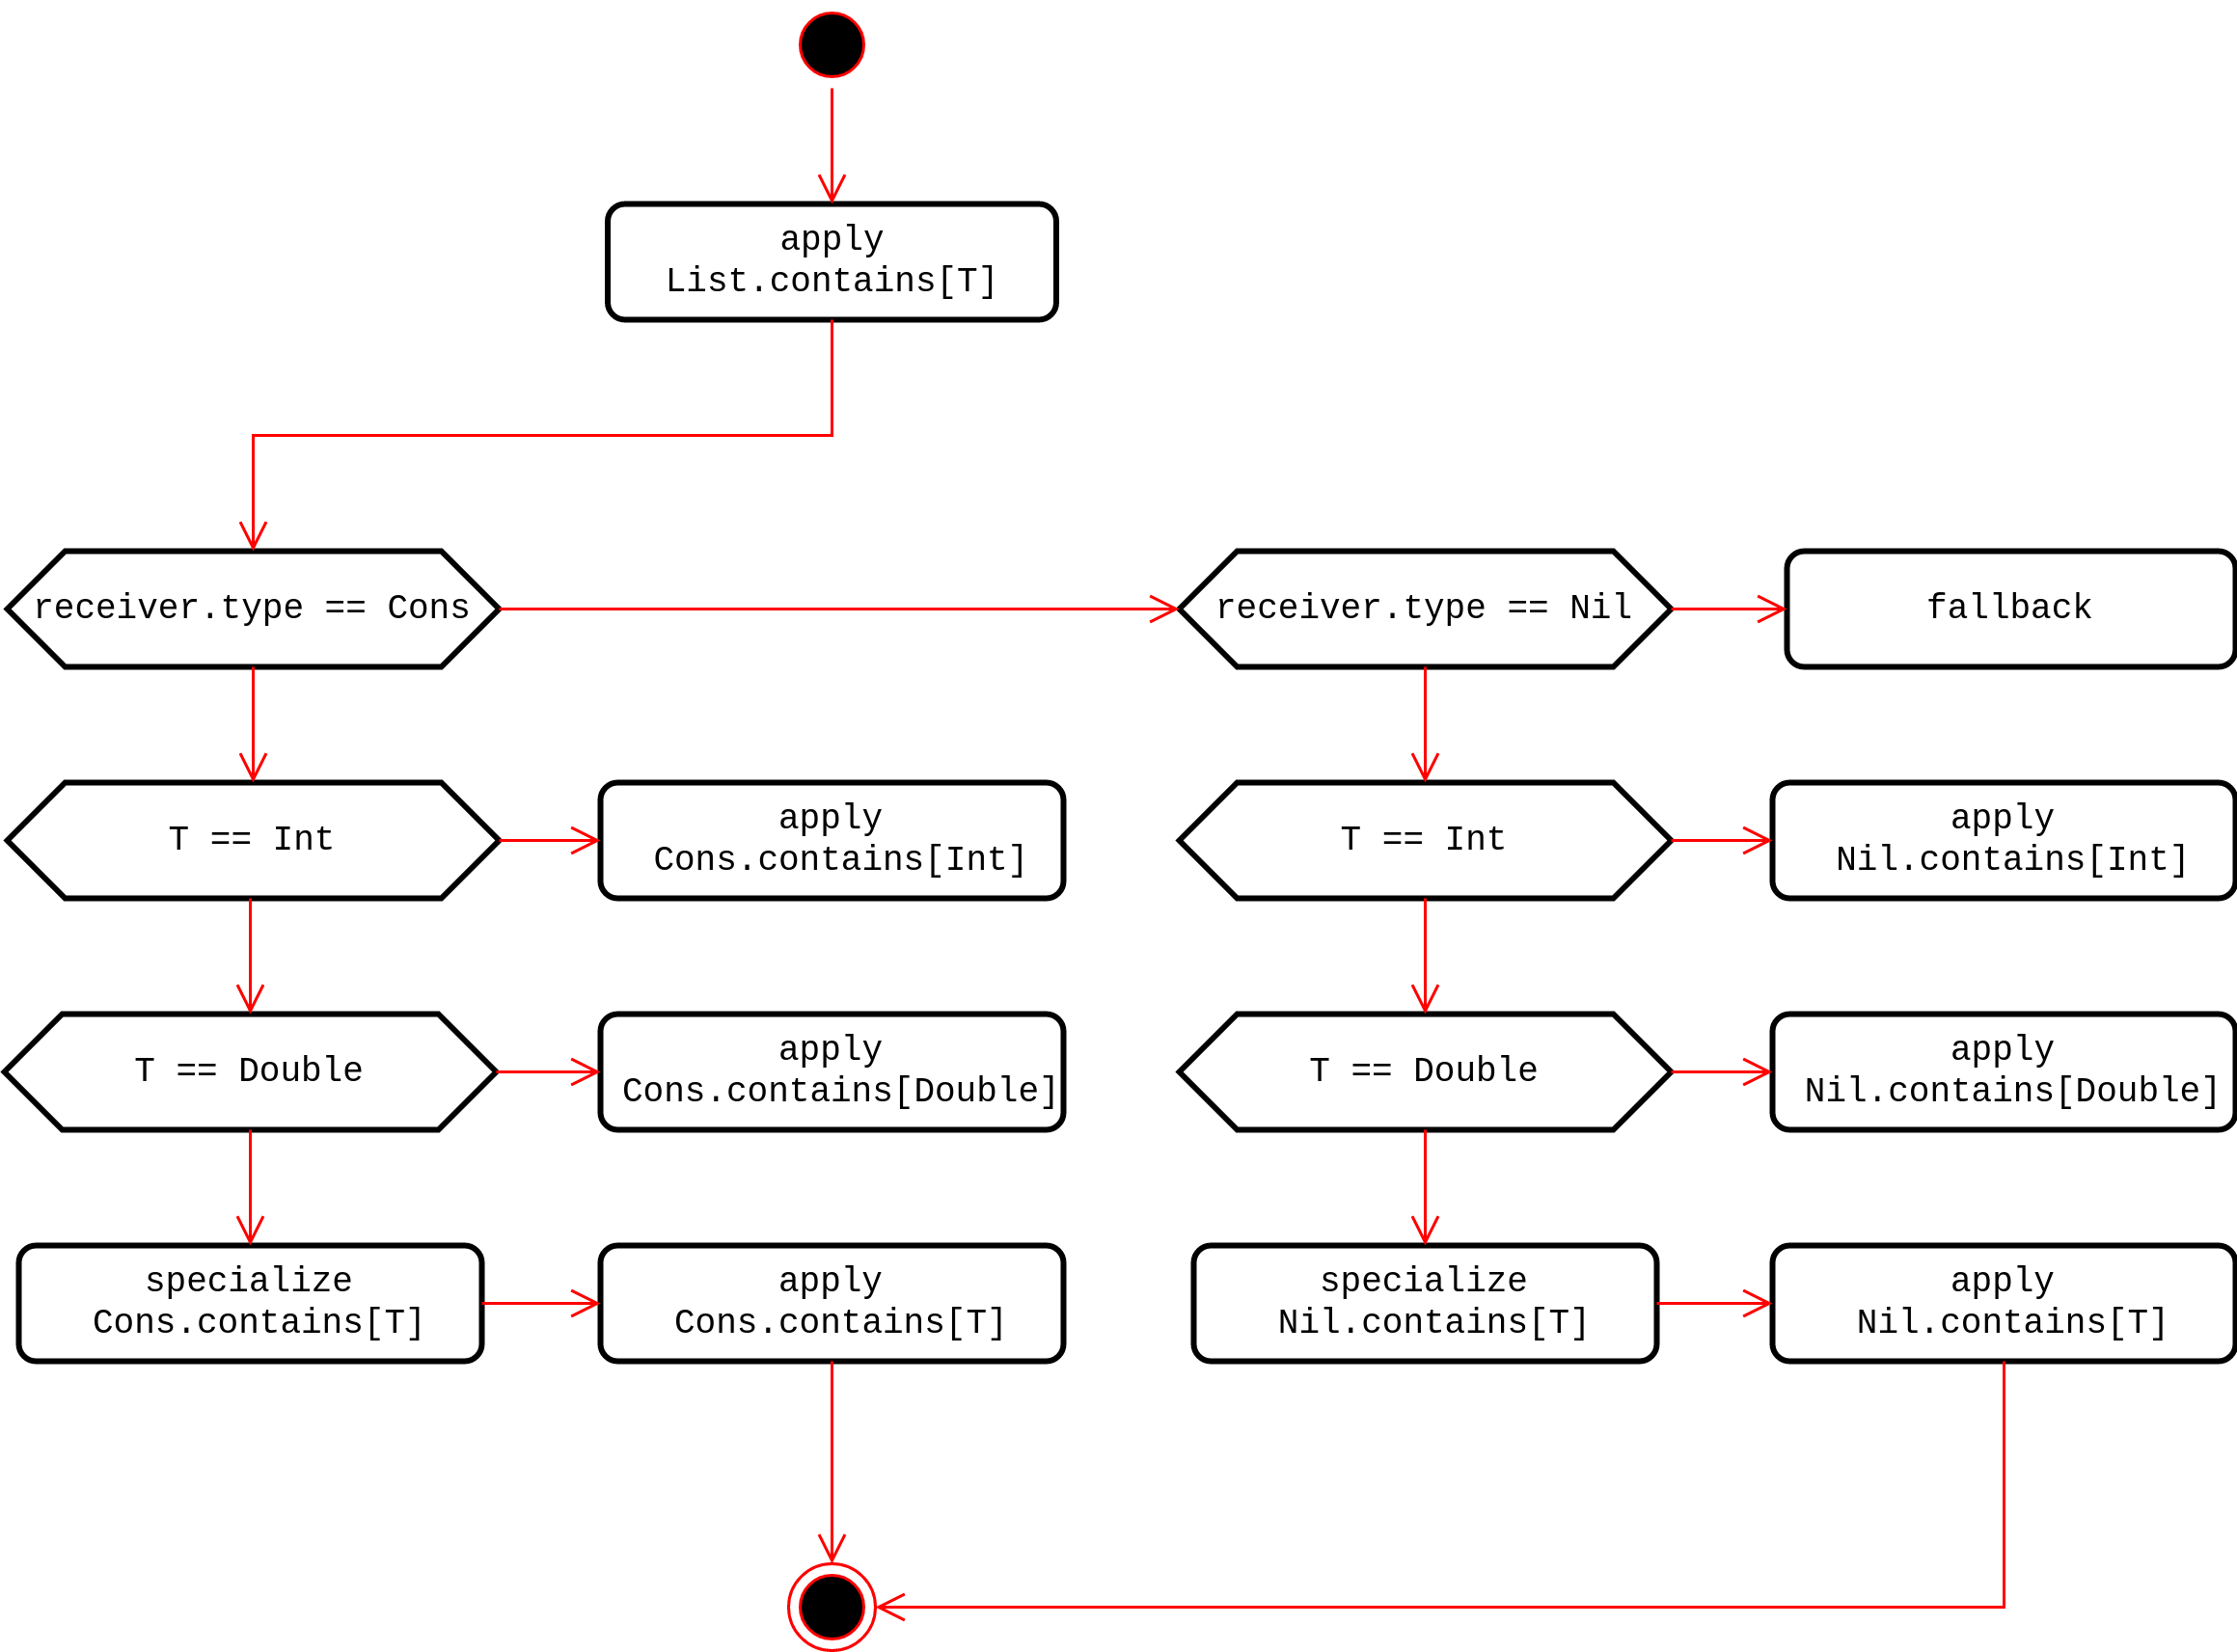
\includegraphics[width=0.75\textwidth]{figures/tastytruffle-type-dispatch-chain.png}
	\caption{The typed dispatch chain for a \scalainline{List.contains} call site}
	\label{example:typed-dispatch}
\end{figure}

Figure \ref{example:typed-dispatch} is an extension of the example given in figure \ref{example:poly-cache-call-node} with typed dispatch.
The example assumes the type arguments for \scalainline{Int} and \scalainline{Double} for \scalainline{Cons.contains[T]} and \scalainline{Nil.contains[T]} has previously been specialized and cached.
After the polymorphic inline cache resolves the receiver to an exact type, the corresponding specialization is looked up.

\subsection{Specializing Classes}

We begin with a discussion on specializing classes as they can only be polymorphic under a single context.
This is in contrast to methods, which can be polymorphic under multiple contexts.
In this section, we specifically focus on specializing classes and their members which solely derive their polymorphic semantics from class type parameters.

\begin{figure}[!htb]
	\begin{minted}{scala}
	class NewNode(@Child typeNode: TypeNode) extends TermNode {
		override def execute(frame: VirtualFrame): Object = {
			val tpe = typeNode.resolveType(frame)
			shapeOf(tpe).newInstance
		}
	}
	\end{minted}
	\caption{The \scalainline{NewNode} for the polymorphic interpreter.}
\end{figure}

\subsubsection*{Case Study: \texttt{Cons.head}}

\begin{figure}[!htb]
	\begin{minted}{scala}
	val list: List[Int] = ???
	list.contains(0)
	\end{minted}
	\caption{Example invocation of \scalainline{Cons.contains[Int]}}
\end{figure}

We introduce an example which will motivate the specialization of storage layouts in shapes.

\begin{figure}[!htb]
	\centering
	\begin{subfigure}[b]{0.4\textwidth}
		\centering
		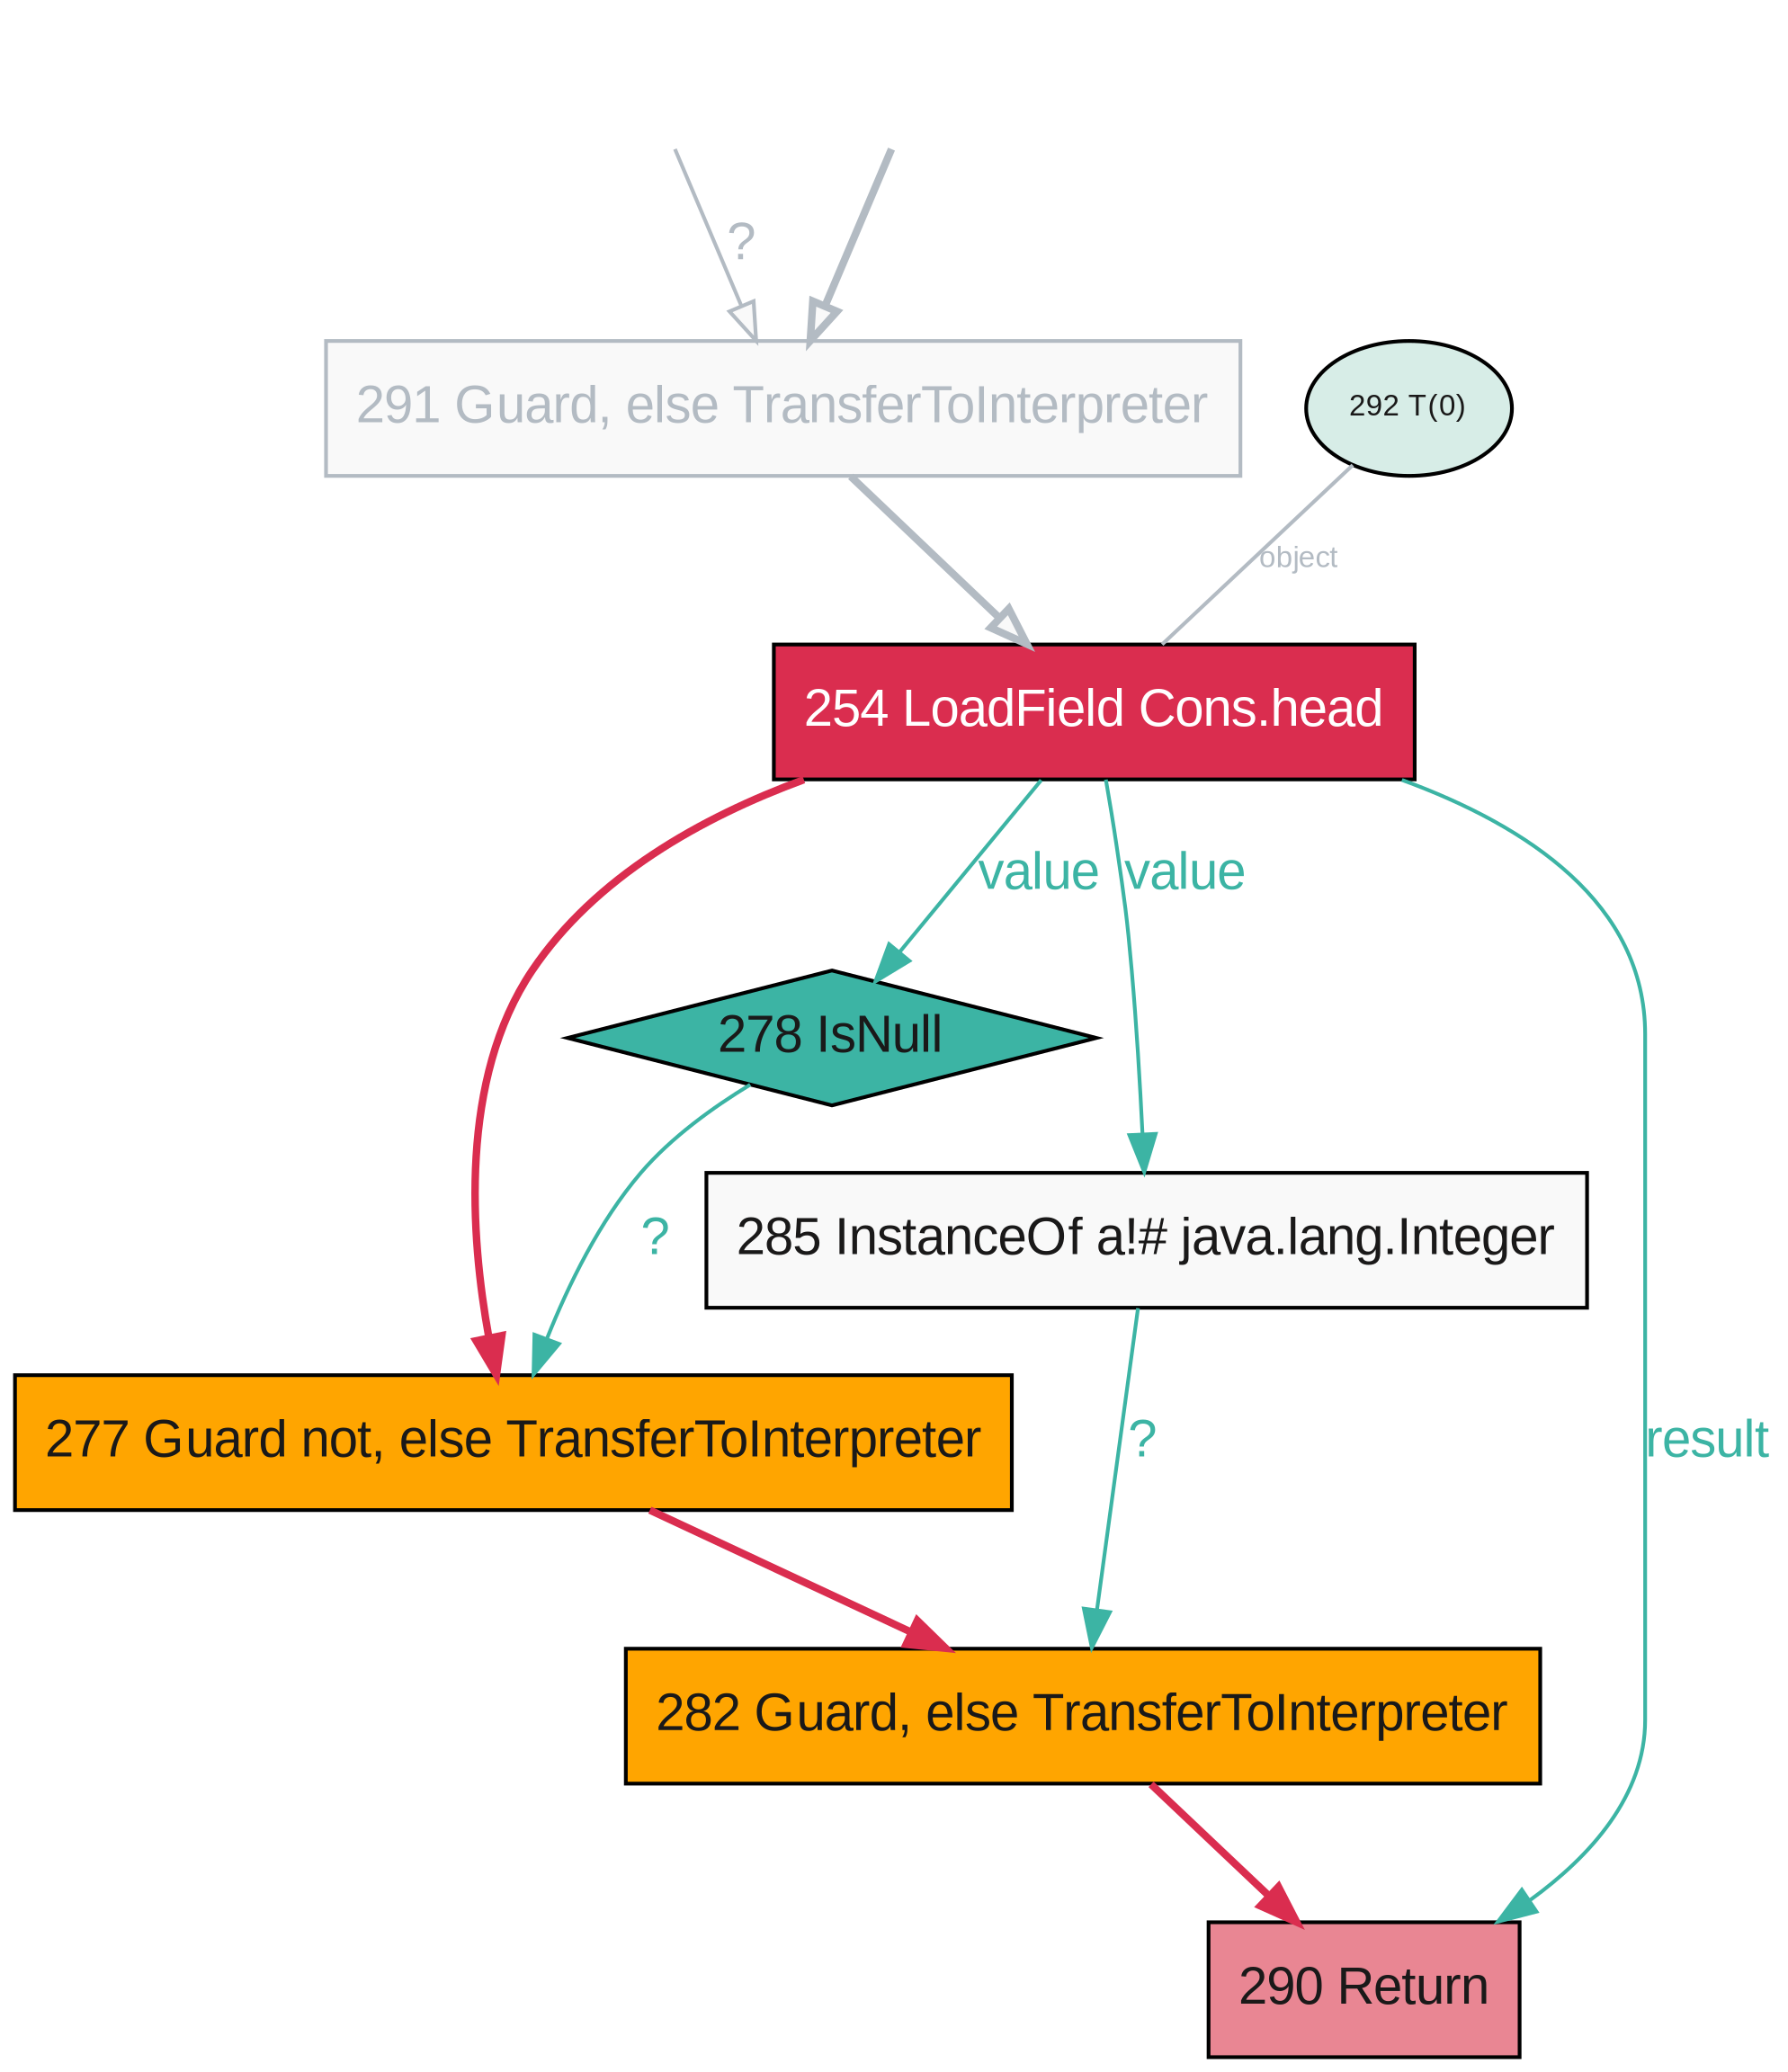
\includegraphics[width=\textwidth]{figures/dot/List.head.boxed.TruffleTier.png}
		\caption{Graal IR of \scalainline{Cons.head} focused on field access of \scalainline{head0}}
		\label{graalir:cons-head-boxed}
	\end{subfigure}
	\hfill
	\begin{subfigure}[b]{0.45\textwidth}
		\centering
		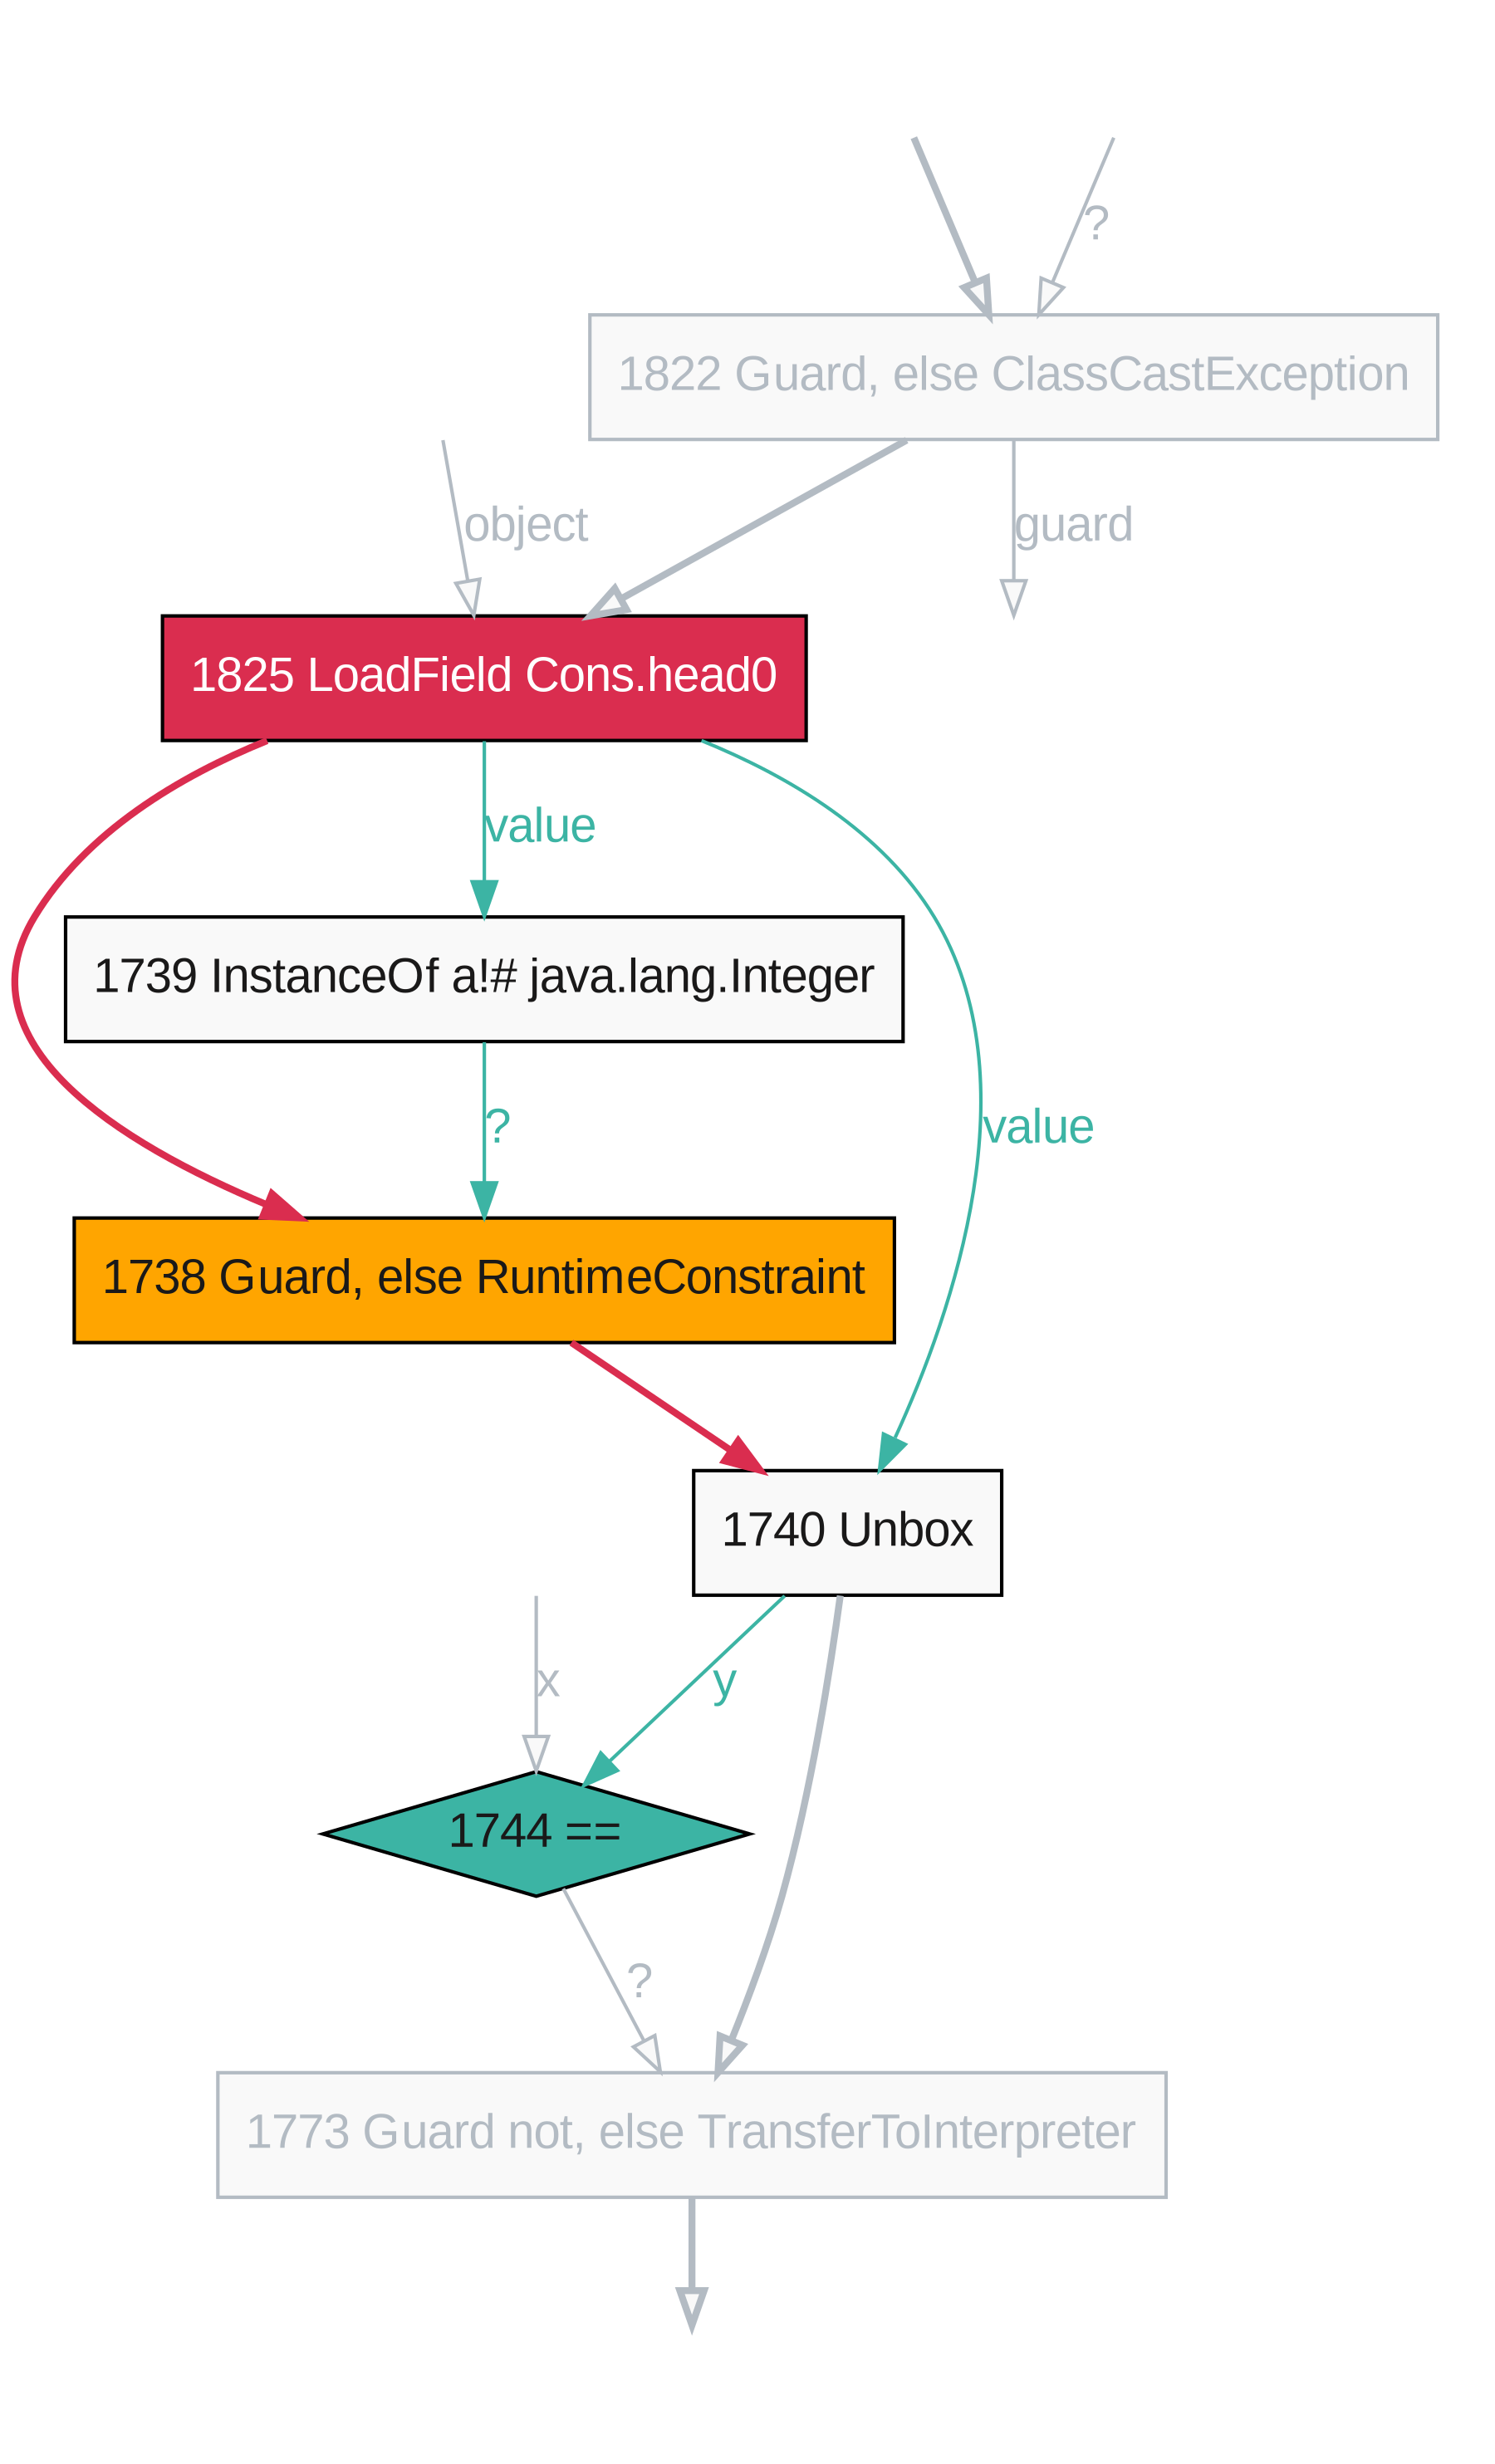
\includegraphics[width=\textwidth]{figures/dot/List.contains.boxed.TruffleTier.png}
		\caption{Graal IR of \scalainline{Cons.head} after being inlined into \scalainline{Cons.contains}}
		\label{graalir:cons-contains-head-focus-boxed}
	\end{subfigure}
	\hfill
\end{figure}

We examine in detail the Graal IR focusing on the \scalainline{List.head} accessor method in our \scalainline{List} running example.
For this particular example, we focus on unboxing that occurs when the \scalainline{head0} is accessed by the \scalainline{List.head}.
This unboxing can be seen in \ref{graalir:cons-head-boxed}.

We can see that \textit{guard} nodes are inserted by Graal into the compiled graph during JIT compilation.
A guard node ensures a speculative assumption still holds during execution.
Because the default storage type of a polymorphic field without specialization is an \javainline{Object}, Graal makes two runtime assumptions about the field in the JIT compiled \scalainline{contains} method to ensure the compiled method does not throw a runtime exception if the return value needs to be unboxed.
The first guard, identifiable by node $278$, checks that the value is not the \javainline{null} reference.
As the \javainline{null} value is only compatible with reference types, attempting to unbox a \javainline{null} value produces a runtime exception.
The second guard, with the identifier $282$, is a type check that the value is an \javainline{Integer} object.
Notice that the predecessor node is the type check \javainline{instanceof a!{\#} java.lang.Integer} and not \javainline{instanceof java.lang.Integer}.
\javainline{instanceof} nodes in Graal IR checks against \textit{stamps} instead of normal JVM types identifiers.
A stamp is much like a type identifier but has additional descriptors attached.
For example, the stamp \javainline{a!{\#} java.lang.Integer} has the following descriptors:

\begin{description}
	\item[\texttt{(a)}] Asserts that the stamp marks a reference type identifier. In the case of this stamp, the stamp marks the boxed reference type \javainline{java.lang.Integer}.
	\item[\texttt{(!)}] Asserts that value is not the \javainline{null} reference value. The stamp contains this descriptor because it is preceded by a non-null guard.
	\item[\texttt{(\#)}] Asserts that value marked by the stamp is \textit{exactly} an instance of the type identifier described by the stamp and not an instance of a subclass of the type identifier
\end{description}

In more succinct terms, the \javainline{instanceof} node $285$ checks that value is precisely the instance of a \javainline{java.lang.Integer} and is not the \javainline{null} value. 
If the assumptions are not violated in compiled code, the boxed integer value is then returned from the compiled code.
Note that no unboxing happens because the value of \scalainline{head0} has not yet been used in a polymorphic context.

When the access or method \scalainline{List.head} is inlined into its callsite in \scalainline{Cons.contains} (see figure \ref{graalir:cons-contains-head-focus-boxed}), an unbox operation is introduced because the equality operation in node $1744$ compares primitives and not references.
Notice that the two guards node previously seen in figure \ref{graalir:cons-head-boxed} are folded into one node because the \javainline{instanceof} node is an extension of the null check node.
Because polymorphic field values are stored as an reference on the object instance, these speculative assumptions are necessary in order to generate compiled code.
To eliminate the overhead of the unbox operation and the accompanying guard nodes, The polymorphic fields of a class must be specialized.

\subsubsection*{Specializing Field Members}

The underlying type of a polymorphic field, and therefore its storage type as part of the shape layout, cannot be determined statically.

\begin{figure}[!htb]
	\begin{minted}{scala}
	class ClassTemplate(
		vdefs: List[ValDef],
		polyDefD: List[],
		methods: List[CallTarget]
	
	) {
		def specialize(types: Array[Type]): ClassShape
	}
	\end{minted}
\end{figure}

\subsubsection*{Specializing Method Members}

\subsubsection*{Creating Specialized Instances}

\subsubsection*{After Specialization}
\begin{figure}[!htb]
	\centering
	\begin{subfigure}[b]{0.4\textwidth}
		\centering
		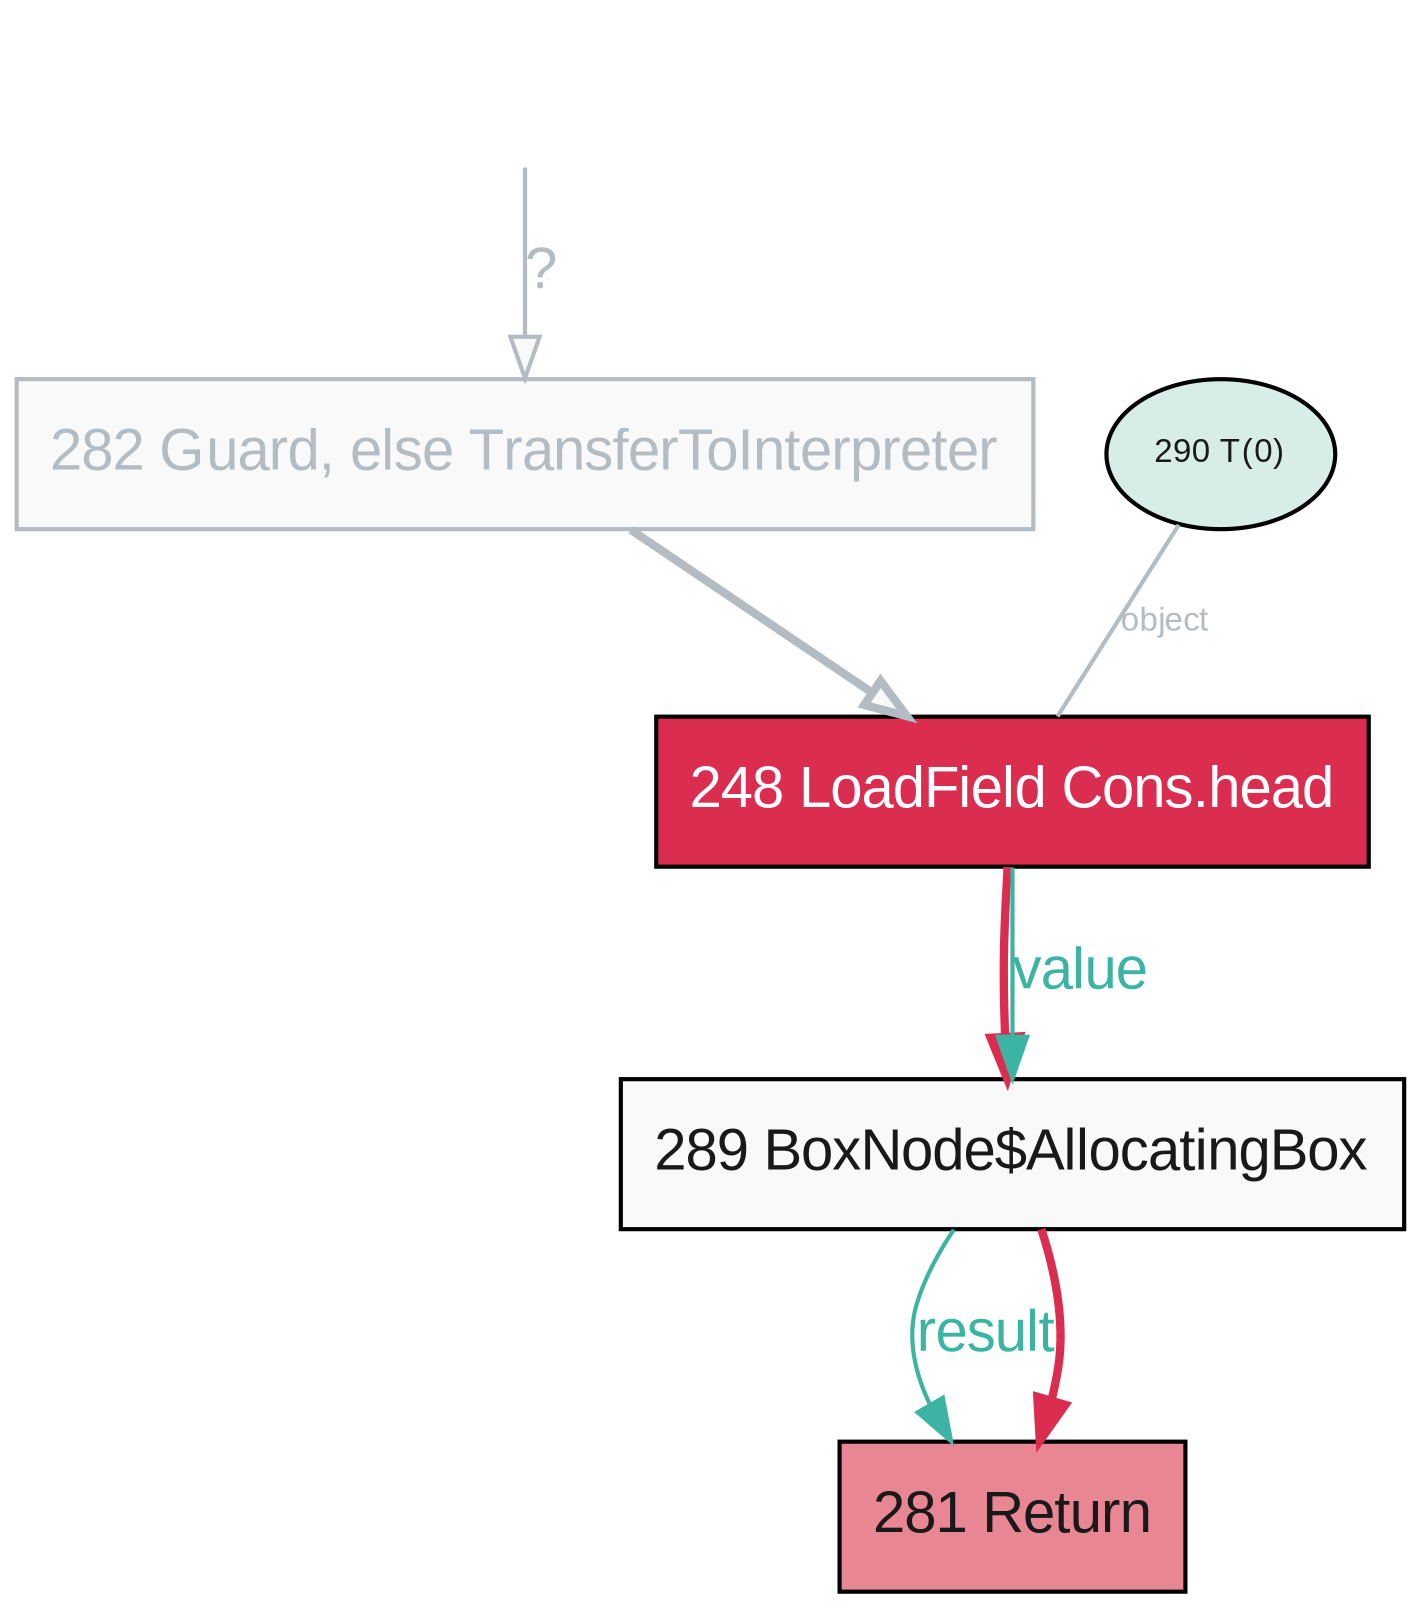
\includegraphics[width=\textwidth]{figures/dot/List.head.specialized.TruffleTier.png}
		\caption{Graal IR of \scalainline{List.head} after field read of \scalainline{head0} is specialized.}
		\label{graalir:cons-head-specialized}
	\end{subfigure}
	\hfill
	\begin{subfigure}[b]{0.4\textwidth}
		\centering
		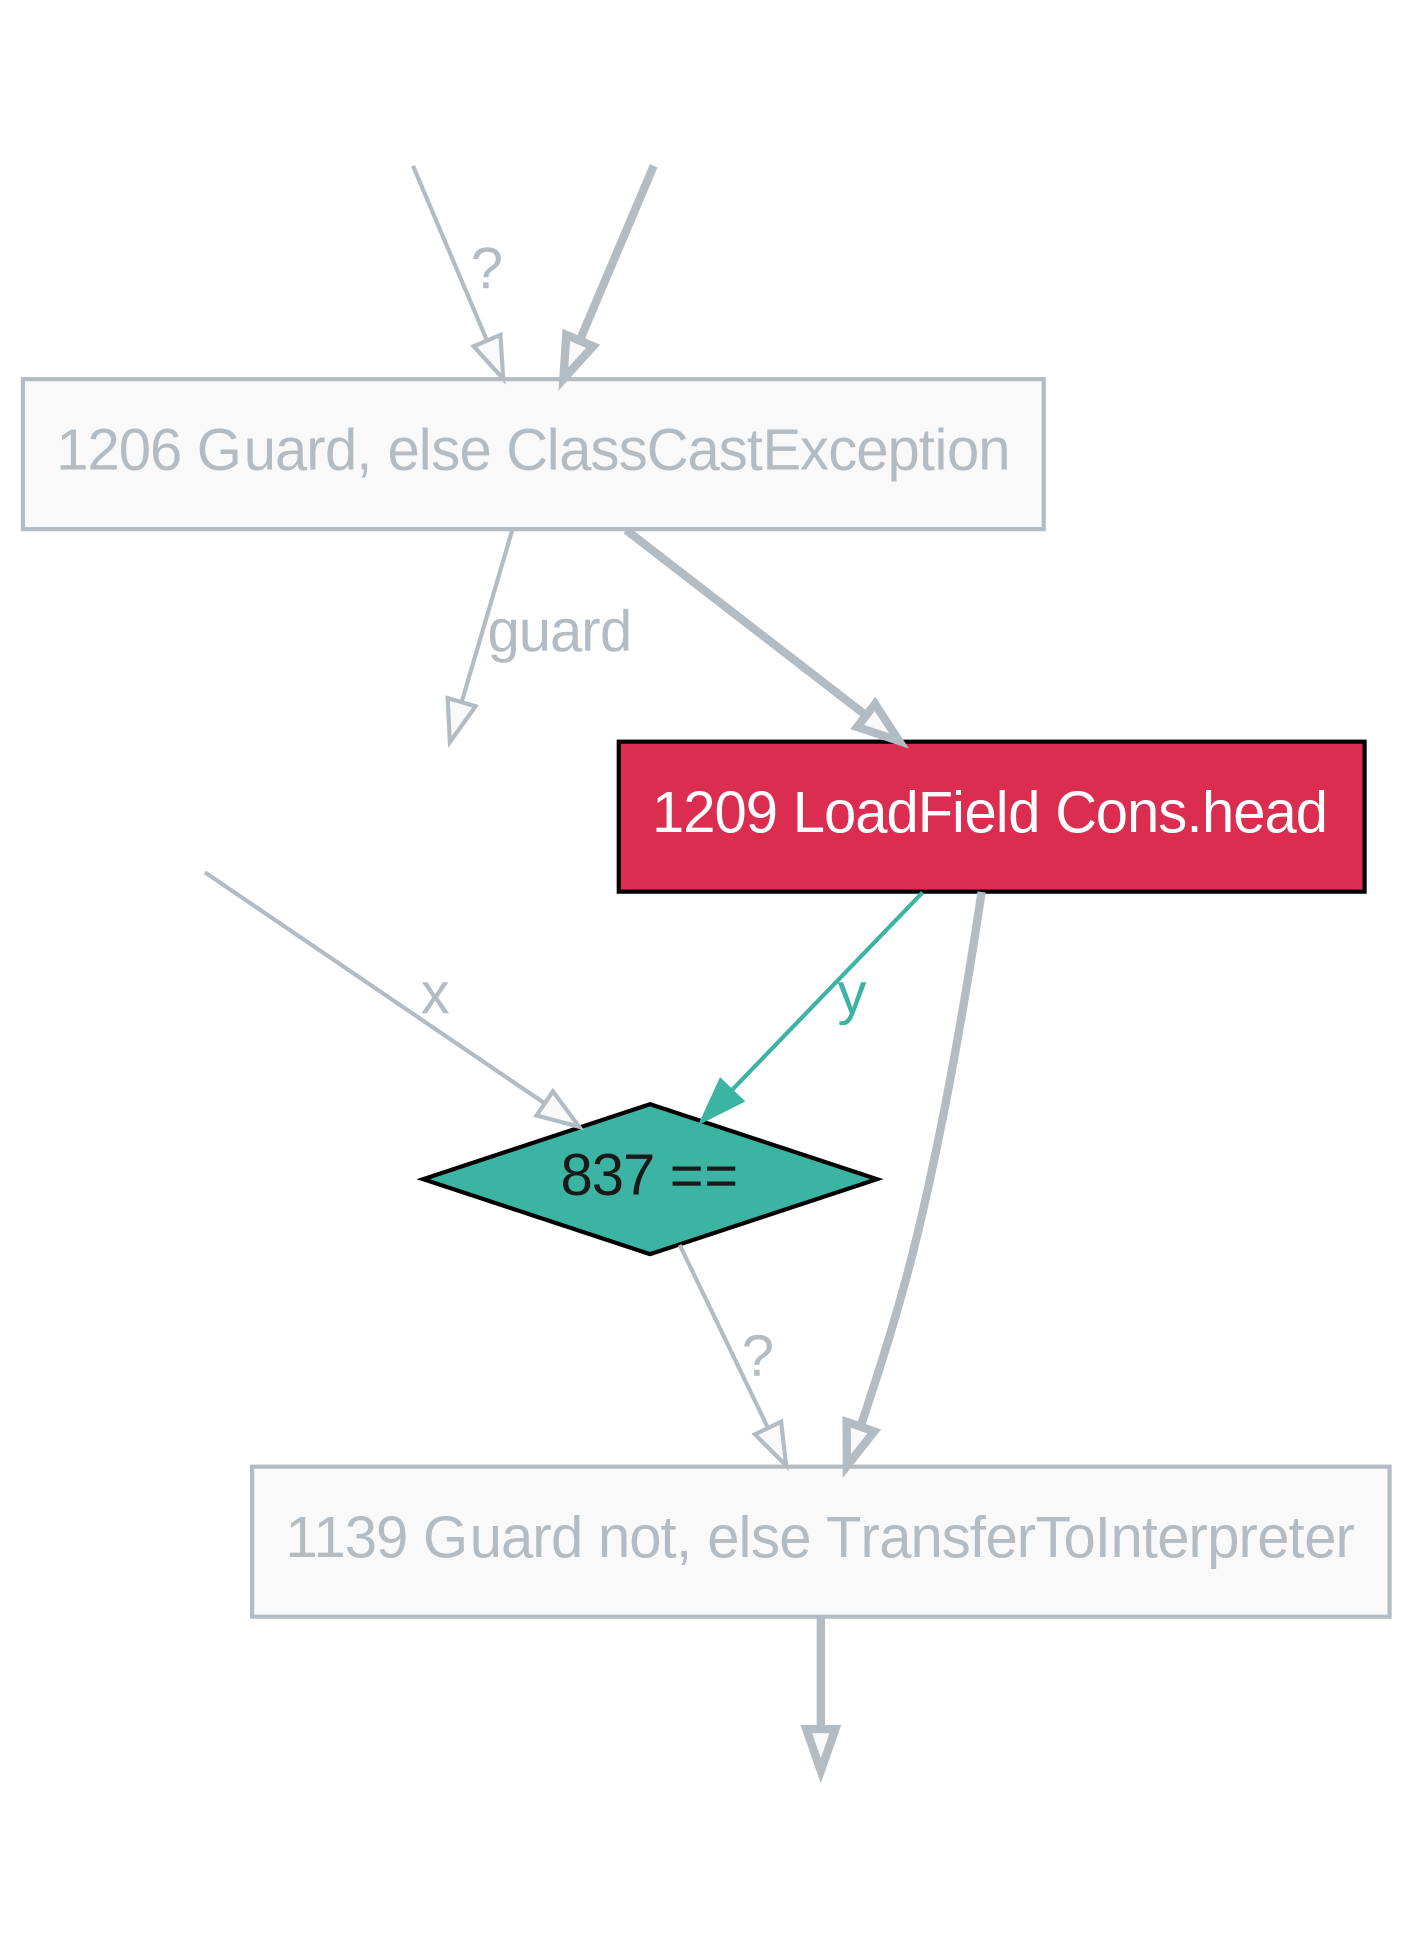
\includegraphics[width=\textwidth]{figures/dot/List.contains.specialized.TruffleTier.png}
		\caption{Graal IR of \scalainline{Cons.head} after being inlined into \scalainline{Cons.contains}}
		\label{graalir:cons-contains-head-focus-specialized}
	\end{subfigure}
	\hfill
\end{figure}

In this section, we will examine previously unboxed code after the specialization of class storage layouts.
Figure \ref{graalir:cons-head-specialized} contains the field access of \scalainline{head0} after the field has been specialized and has the appropriate storage type in the storage layout of \scalainline{Cons[Int]}.
Notice that a box node has been introduced prior to the value of \scalainline{head0} prior to the return node of \scalainline{Cons.head}.
Because the \scalainline{execute} method of a \scalainline{DefDefNode} returns an \javainline{Object}, the return value is preemptively boxed when inspecting the IR of the method.
However, after inlining into the body of \scalainline{Cons.contains}, the box operation is no longer necessary as the boxed value will be immediately unboxed.
Graal will automatically eliminate this type of autoboxing.
When a specialized class instance is used in place of a generic class instance, the field access graph of \scalainline{head0} is the simplest possible graph.



%======================================================================

\chapter{Evaluation}

%======================================================================


\chapter{Related Work}

This chapter discusses previous academic and industrial work related to this thesis. 
The first section provides an introduction to the various implementations of parametric polymorphism.
The second section covers related work on the implementation of polymorphism in Java.
The third section of this chapter provides an overview of previous and state-of-the-art efforts to specialize Scala programs.
The last section presents prior and ongoing efforts in the implementation of other Truffle interpreters.

\section{Implementations of Parametric Polymorphism}

Implementations of parametric polymorphism can be divided into two broad categories\cite{java:odersky-type-params}:

\begin{description}
	\item[\textit{Homogeneous Translation}] 
	This approach provides a single data representation for each polymorphic type. 
	An example of this implementation is the type erasure transformation applied in the Java and Scala compilation pipelines.
	Morrison et al. also refer to this form of polymorphism as the \scalainline{uniform polymorphism}\cite{types-of-polymorphism}.
	\item[\textit{Heterogeneous Translation}]
	In contrast to homogeneous translation, the heterogeneous translation ensures a unique data representation for every polymorphic type instantiation.The heterogeneous translation can also be referred to as \textit{textual polymorphism}.
\end{description}

This section will cover various approaches to implementing parametric polymorphism in the context of these two forms.
As polymorphism in Java and Scala are more relevant to the central themes of this thesis, we will first focus on implementations of parametric polymorphism for other languages.

Parametric polymorphism was first studied in functional programming languages\cite{ml:parametric-polymorphism}\cite{ml:type-inference}.
Leroy proposed an approach in which type coercion operations are inserted between polymorphic operations and monomorphic data. 
The coercion operations in this approach are quite similar to the notion of boxing and unboxing, which Leroy describes as \textit{wrapping} and \textit{unwrapping}.

The heterogeneous translation is the more prevalent implementation of parametric polymorphism in object-oriented programming languages.
The \mintinline{cpp}|template| concept in the \CC\ programming language popularized parametric polymorphism in objected-oriented programming languages.
Templates define a generic definition of some kind in \CC.
The \CC\ compiler will generate heterogeneous translations based on every set of concrete type arguments supplied during compilation.
The implementation of polymorphism in the Common Language Runtime\cite{clr:overview}\cite{clr:spec} by Kennedy and Syme makes use of reified types in a polymorphic bytecode IR during execution.
Polymorphic class definitions are loaded as templates; Templates generate specialized class layouts on an ad-hoc basis based on the reified type arguments seen during bytecode execution.
Their approach relies on CLR extensions to support types not present in existing JVM implementations.
Our approach shares many similarities with the approach described by Kennedy and Syme.
One drawback of their approach is that the polymorphic bytecode IR does not support the complete set of operations on types.
For example, reflection is necessary to differentiate between a \scalainline{List[Int]} and a \scalainline{List[String]}.
Our implementation differs as such operations are possible because the IR could potentially incorporate the full type language of TASTy.

\section{Generics and Java}

Prior efforts to implement generics in Java have been based on static compilation techniques restricted by the \textit{open world assumption}.
The open world assumption is an assumption that the program under compilation is \textit{incomplete}; extra parts of the program will be supplied in a future iteration of compilation.
This form of compilation is commonly known as \textit{separate compilation}.
As such, the compilation results of the current parts of the program must be interoperable with the compilation results of the remaining yet-to-be-determined parts.

The Java language did not initially support parametric polymorphism in its initial release.
As a result, many different approaches were proposed before a uniform polymorphism became the accepted implementation for Java.
Pizza\cite{java:pizza} was a superset of Java that supported heterogeneous and homogeneous translations of polymorphic definitions into Java.
Agesen, Freund, and Mitchell proposed a heterogeneous translation for parametric polymorphism for Java during load-time instead of compile-time\cite{java:agesen-type-params}.
NextGen\cite{java:nextgen} separates the translation of polymorphic classes into monomorphic and polymorphic components.
In NextGen, Only the polymorphic members of a class definition are specialized; These specialized classes inherit the implementation of their monomorphic members from a common parent class.
Finally, GJ\cite{java:gj} proposed the foundations for what is now the accepted implementation of parametric polymorphism in Java.
Polymorphic class definitions have a single uniform data representation after type erasure.
These approaches determine the data representation of polymorphic definitions in a static context.
Our approach is based on the \textit{closed world assumption} as the entire program must be available in order for it to be executed.

\section{Specialization in Scala}

The standard implementation of parametric polymorphism follows that of Java; generic class definitions have their type parameters erased.
All previous approaches attempt to avoid the problem of bytecode explosion, where the specialization of polymorphic data with every possible type creates an exponential number of unique data representations.
Dragos describes the earliest efforts to specialize Scala programs with the aid of annotations\cite{scala:specialization}.
Annotations avoid unnecessarily specializing polymorphic data through knowledge injected by a programmer.
Ureche, Talau, and Odersky expand upon this approach by reducing unnecessary duplication among specializations through sharing\cite{scala:miniboxing}.
Sharing exploits the insight that specializations of some value types may be reused for the specializations of other value types.
For example, the representation of \scalainline{ArrayBuffer[Long]} could be used, with the addition of some glue code, for the specialization of \scalainline{ArrayBuffer[Int]} instead of generating an additional specialized representation. 
Both approaches mix the implementation of uniform polymorphism with user-guided specialization directives.
Our generates a heterogeneous translation of a generic class definition on an ad-hoc basis;

\section{Truffle Interpreters}

There are many Truffle interpreters in active development at the time of writing.
This section will attempt to provide a brief survey of Truffle interpreters.
TruffleRuby\cite{trufflyruby:specialization}\cite{truffleruby:object-model},FastR, Graal.js, Graal.Python,\cite{truffle:thesis} are some of the industrial implementations of dynamically typed languages implemented with Truffle.
They all make substantial use of Truffle facilities, some discussed earlier in this thesis, to speculative optimize program execution. 
Espresso\cite{graalvm: espresso} is an implementation of a Java bytecode interpreter in Truffle. 
Espresso is a metacircular implementation of a Java Virtual Machine.
Because Espresso executes the same Java bytecode format as other JVM implementations, it uses the same approaches to optimizing polymorphic data layout as the conventional implementation of Java on GraalVM.




%======================================================================

%======================================================================
\chapter{Future Work}
%======================================================================


%======================================================================
\chapter{Conclusions}
%======================================================================

%----------------------------------------------------------------------
% END MATERIAL
%----------------------------------------------------------------------

% B I B L I O G R A P H Y
% -----------------------

% The following statement selects the style to use for references.  It controls the sort order of the entries in the bibliography and also the formatting for the in-text labels.
\bibliographystyle{plain}
% This specifies the location of the file containing the bibliographic information.  
% It assumes you're using BibTeX (if not, why not?).
\cleardoublepage % This is needed if the book class is used, to place the anchor in the correct page,
                 % because the bibliography will start on its own page.
                 % Use \clearpage instead if the document class uses the "oneside" argument
\phantomsection  % With hyperref package, enables hyperlinking from the table of contents to bibliography             
% The following statement causes the title "References" to be used for the bibliography section:
\renewcommand*{\bibname}{References}

% Add the References to the Table of Contents
\addcontentsline{toc}{chapter}{\textbf{References}}

\bibliography{uw-ethesis}
% Tip 5: You can create multiple .bib files to organize your references. 
% Just list them all in the \bibliogaphy command, separated by commas (no spaces).

% The following statement causes the specified references to be added to the bibliography% even if they were not 
% cited in the text. The asterisk is a wildcard that causes all entries in the bibliographic database to be included (optional).
\nocite{*}

% The \appendix statement indicates the beginning of the appendices.
\appendix
% Add a title page before the appendices and a line in the Table of Contents
\chapter*{APPENDICES}
\addcontentsline{toc}{chapter}{APPENDICES}

\chapter{Scala 3 Compiler Phases}
\label{appendix:dotty-phases}
\begin{minted}{scala}
	/** Phases dealing with the frontend up to trees ready for TASTY pickling */
	protected def frontendPhases: List[List[Phase]] =
		List(new Parser) ::                       // scanner, parser
		List(new TyperPhase) ::                   // namer, typer
		List(new YCheckPositions) ::              // YCheck positions
		List(new sbt.ExtractDependencies) ::      // Sends information on classes' dependencies to sbt via callbacks
		List(new semanticdb.ExtractSemanticDB) :: // Extract info into .semanticdb files
		List(new PostTyper) ::                    // Additional checks and cleanups after type checking
		List(new sjs.PrepJSInterop) ::            // Additional checks and transformations for Scala.js (Scala.js only)
		List(new Staging) ::                      // Check PCP, heal quoted types and expand macros
		List(new sbt.ExtractAPI) ::               // Sends a representation of the API of classes to sbt via callbacks
		List(new SetRootTree) ::                  // Set the `rootTreeOrProvider` on class symbols
		Nil
\end{minted}

\begin{minted}{scala}
	/** Phases dealing with TASTY tree pickling and unpickling */
	protected def picklerPhases: List[List[Phase]] =
		List(new Pickler) ::            // Generate TASTY info
		List(new PickleQuotes) ::       // Turn quoted trees into explicit run-time data structures
		Nil
\end{minted}

\begin{minted}{scala}
	/** Phases dealing with the transformation from pickled trees to backend trees */
	protected def transformPhases: List[List[Phase]] =
		List(
			new FirstTransform,         // Some transformations to put trees into a canonical form
			new CheckReentrant,         // Internal use only: Check that compiled program has no data races involving global vars
			new ElimPackagePrefixes,    // Eliminate references to package prefixes in Select nodes
			new CookComments,           // Cook the comments: expand variables, doc, etc.
			new CheckStatic,            // Check restrictions that apply to @static members
			new BetaReduce,             // Reduce closure applications
			new init.Checker) ::        // Check initialization of objects
		List(
			new ElimRepeated,           // Rewrite vararg parameters and arguments
			new ExpandSAMs,             // Expand single abstract method closures to anonymous classes
			new ProtectedAccessors,     // Add accessors for protected members
			new ExtensionMethods,       // Expand methods of value classes with extension methods
			new UncacheGivenAliases,    // Avoid caching RHS of simple parameterless given aliases
			new ByNameClosures,         // Expand arguments to by-name parameters to closures
			new HoistSuperArgs,         // Hoist complex arguments of supercalls to enclosing scope
			new SpecializeApplyMethods, // Adds specialized methods to FunctionN
			new RefChecks) ::           // Various checks mostly related to abstract members and overriding
		List(
		 	// Turn opaque into normal aliases
			new ElimOpaque,            
			// Compile cases in try/catch
			new TryCatchPatterns,      
			// Compile pattern matches
			new PatternMatcher,         
			// Make all JS classes explicit (Scala.js only)
			new sjs.ExplicitJSClasses,  
			// Add accessors to outer classes from nested ones.
			new ExplicitOuter,          
			// Make references to non-trivial self types explicit as casts
			new ExplicitSelf,           
			// Expand by-name parameter references
			new ElimByName,             
			// Optimizes raw and s string interpolators by rewriting them to string concatentations
			new StringInterpolatorOpt) :: 
		List(
			new PruneErasedDefs,        // Drop erased definitions from scopes and simplify erased expressions
			new InlinePatterns,         // Remove placeholders of inlined patterns
			new VCInlineMethods,        // Inlines calls to value class methods
			new SeqLiterals,            // Express vararg arguments as arrays
			new InterceptedMethods,     // Special handling of `==`, `|=`, `getClass` methods
			new Getters,                // Replace non-private vals and vars with getter defs (fields are added later)
			new SpecializeFunctions,    // Specialized Function{0,1,2} by replacing super with specialized super
			new LiftTry,                // Put try expressions that might execute on non-empty stacks into their own methods
			new CollectNullableFields,  // Collect fields that can be nulled out after use in lazy initialization
			new ElimOuterSelect,        // Expand outer selections
			new ResolveSuper,           // Implement super accessors
			new FunctionXXLForwarders,  // Add forwarders for FunctionXXL apply method
			new ParamForwarding,        // Add forwarders for aliases of superclass parameters
			new TupleOptimizations,     // Optimize generic operations on tuples
			new LetOverApply,           // Lift blocks from receivers of applications
			new ArrayConstructors) ::   // Intercept creation of (non-generic) arrays and intrinsify.
		List(new Erasure) ::            // Rewrite types to JVM model, erasing all type parameters, abstract types and refinements.
		List(
			new ElimErasedValueType,    // Expand erased value types to their underlying implmementation types
			new PureStats,              // Remove pure stats from blocks
			new VCElideAllocations,     // Peep-hole optimization to eliminate unnecessary value class allocations
			new ArrayApply,             // Optimize `scala.Array.apply([....])` and `scala.Array.apply(..., [....])` into `[...]`
			new sjs.AddLocalJSFakeNews, // Adds fake new invocations to local JS classes in calls to `createLocalJSClass`
			new ElimPolyFunction,       // Rewrite PolyFunction subclasses to FunctionN subclasses
			new TailRec,                // Rewrite tail recursion to loops
			new CompleteJavaEnums,      // Fill in constructors for Java enums
			new Mixin,                  // Expand trait fields and trait initializers
			// Expand lazy vals
			new LazyVals,              
			// Add private fields to getters and setters
			new Memoize,                
			 // Expand non-local returns
			new NonLocalReturns,       
			// Represent vars captured by closures as heap objects
			new CapturedVars) ::        
		List(
			new Constructors,           // Collect initialization code in primary constructors
			// Note: constructors changes decls in transformTemplate, no InfoTransformers should be added after it
			new Instrumentation) ::     // Count calls and allocations under -Yinstrument
		List(
			// Lifts out nested functions to class scope, storing free variables in environments
			new LambdaLift,             
			// Note: in this mini-phase block scopes are incorrect. No phases that rely on scopes should be here
			// Replace `this` references to static objects by global identifiers
			new ElimStaticThis,         
			// Identify outer accessors that can be dropped
			new CountOuterAccesses) :: 
		List(
			// Drop unused outer accessors
			new DropOuterAccessors,     
			// Lift all inner classes to package scope
			new Flatten,                
			// Renames lifted classes to local numbering scheme
			new RenameLifted,           
			// Replace wildcards with default values
			new TransformWildcards,     
			 // Move static methods from companion to the class itself
			new MoveStatics,           
			// Widen private definitions accessed from nested classes
			new ExpandPrivate,          
			 // Repair scopes rendered invalid by moving definitions in prior phases of the group
			new RestoreScopes,         
			// get rid of selects that would be compiled into GetStatic
			new SelectStatic,           
			// Generate JUnit-specific bootstrapper classes for Scala.js (not enabled by default)
			new sjs.JUnitBootstrappers, 
			// Find classes that are called with super
			new CollectSuperCalls) ::   
		Nil
\end{minted}

\begin{minted}{scala}
	/** Generate the output of the compilation */
	protected def backendPhases: List[List[Phase]] =
		List(new backend.sjs.GenSJSIR) :: // Generate .sjsir files for Scala.js (not enabled by default)
		List(new GenBCode) ::             // Generate JVM bytecode
		Nil
\end{minted}
%======================================================================

\end{document}
